%%%%%%%%%%%%%%%%%%%%%%%%%%%%%%%%%%%%%%%%%
%%            LMU-Vorlage              %%
%%                                     %%
%%         zur Erstellung einer        %%
%%   Dissertation mit pdflatex/latex   %%
%%                                     %%
%%  (2002) Robert Dahlke               %%
%%         & Sigmund Stintzing         %%
%%%%%%%%%%%%%%%%%%%%%%%%%%%%%%%%%%%%%%%%%

\documentclass[12pt]{book}


%%%%%%%%%%%%%%%%%%%%%%%%%%%%
%%   Zusaetzliche Pakete  %%
%%%%%%%%%%%%%%%%%%%%%%%%%%%%

\usepackage{a4wide}
\usepackage{fancyhdr}
\usepackage{graphicx}
%\usepackage{german}
\usepackage[bookmarks]{hyperref}
\usepackage{amsmath}

%%%%%%%%%%%%%%%%%%%%%%%%%%%%%%
%% Definition der Kopfzeile %%
%%%%%%%%%%%%%%%%%%%%%%%%%%%%%%

\pagestyle{fancyplain}
\renewcommand{\chaptermark}[1]%
         {\markboth{\thechapter.\ #1}{}}
\renewcommand{\sectionmark}[1]%
         {\markright{\thesection\ #1}}
\lhead[\fancyplain{}{\bfseries\thepage}]%
    {\fancyplain{}{\bfseries\rightmark}}
\rhead[\fancyplain{}{\bfseries\leftmark}]%
    {\fancyplain{}{\bfseries\thepage}}
\cfoot{}


%%%%%%%%%%%%%%%%%%%%%%%%%%%%%%%%%%%%%%%%%%%%%%%%%%%%%
%%  Definition des Deckblattes und der Titelseite  %%
%%%%%%%%%%%%%%%%%%%%%%%%%%%%%%%%%%%%%%%%%%%%%%%%%%%%%

\newcommand{\LMUTitle}[9]{
  \thispagestyle{empty}
  \vspace*{\stretch{1}}
  {\parindent0cm
   \rule{\linewidth}{.7ex}}
  \begin{flushright}

    \vspace*{\stretch{1}}
    \sffamily\bfseries\Huge
    #1\\
    \vspace*{\stretch{1}}
    \sffamily\bfseries\large
    #2
    \vspace*{\stretch{1}}
  \end{flushright}
  \rule{\linewidth}{.7ex}
  \vspace*{\stretch{5}}
  \begin{center}
    
\includegraphics[width=2in]{siegel}
  \end{center}
  \vspace*{\stretch{1}}
  \begin{center}\sffamily\LARGE{#5}\end{center}
  \newpage
  \thispagestyle{empty}

  \cleardoublepage
  \thispagestyle{empty}

  \vspace*{\stretch{1}}
  {\parindent0cm
  \rule{\linewidth}{.7ex}}
  \begin{flushright}
    \vspace*{\stretch{1}}
    \sffamily\bfseries\Huge
    #1\\
    \vspace*{\stretch{1}}
    \sffamily\bfseries\large
    #2
    \vspace*{\stretch{1}}
  \end{flushright}
  \rule{\linewidth}{.7ex}

  \vspace*{\stretch{3}}
  \begin{center}
    \Large Dissertation\\
    \Large an der #4\\
    \Large der Ludwig--Maximilians--Universit\"{a}t\\
    \Large M\"unchen\\
    \vspace*{\stretch{1}}
    \Large vorgelegt von\\
    \Large #2\\
    \Large aus #3\\
    \vspace*{\stretch{2}}
    \Large M\"unchen, den #6
  \end{center}

  \newpage
  \thispagestyle{empty}

  \vspace*{\stretch{1}}

  \begin{flushleft}
    \large Erstgutachter:  #7 \\[1mm]
    \large Zweitgutachter: #8 \\[1mm]
    \large Tag der m\"{u}ndlichen Pr\"{u}fung: #9\\
  \end{flushleft}

  \cleardoublepage
}




%%%%%%%%%%%%%%%%%%%%%%%%%%%%
%%  Beginn des Dokuments  %%
%%%%%%%%%%%%%%%%%%%%%%%%%%%%

\begin{document}


  \frontmatter


  \LMUTitle
      {Modelling Internally Coupled Ears
       }               % Titel der Arbeit
      {Anupam Prasad Vedurmudi}                       % Vor- und Nachname des Autors
      {Kolkata, Indien}                             % Geburtsort des Autors
      {Fakult\"{a}t f\"{u}r Physik}                         % Name der Fakultaet
      {M\"{u}nchen 2013}                          % Ort und Jahr der Erstellung
      {\today}                            % Tag der Abgabe
      {Prof. Dr. J. Leo van Hemmen}                          % Name des Erstgutachters
      {Zweitgutachter}                         % Name des Zweitgutachters
      {Pr\"ufungsdatum}                         % Datum der muendlichen Pruefung


  \tableofcontents
  \markboth{Table of Contents}{Table of Contents}


  \listoffigures
  \markboth{List of Figures}{List of Figures}


  \listoftables
  \markboth{List of Tables}{List of Tables}
  \cleardoublepage


  \markboth{Abstract}{Abstract}
  \addcontentsline{toc}{chapter}{\protect Abstract}


\chapter*{Abstract}

ICE is a general model for the production of directional cues in hearing in animals with
tympani that are coupled through the mouth cavity. We first describe the geometric model
for such a system as a cylindrical air cavity closed on either end by linear elastic sectoral 
membranes, i.e. circular membranes with one rigid non-moving sector.


  \mainmatter\setcounter{page}{1}
  \chapter{Introduction}\label{introchapter}
The auditory system is among the most ubiquitious of sensory systems as evidenced by the 
development of numerous strategies for the detection and processing of auditory stimuli
across several species. The processing of sound stimuli is fairly fast and in comparison
to light stimuli, sound has two main properties - it is omnidirectional and due to
its large wavelength, it isn't blocked by small objects. For instance we can hear objects
behind us or behind obstacles whereas the same isn't true for visual stimuli. These properties 
give the animal the obvious advantage of being able to react to approaching dangers that
aren't yet visible. In order to fully utilize the sound stimuli, it is therefore essential
that an animal is able to assess the direction or, to use the technical term, \textit{localize} a sound source.

Before we discuss the various sound localization methods observed in nature, we first
go through the fundamental steps involved in auditory perception. First, an object generates
an auditory stimulus which in general can be very complex. This stimulus then propagates
through a given medium (e.g. air, water) and excites the primary receiver(s) of the animal. In most
terrestrial vertebrates, these take the form of \textit{tympani} or eardrums - a pair of thin vibrating
membranes which are a component of the mechanical part of the auditory system.
Depending on the species, there may be an apparatus that focuses and amplifies the sound waves. In
humans for example, this function performed by the external ears or pinnae. 
The vibrations are then transmitted by means of a set of bony or cartilaginous elements and
converted into electrochemical signals that will be processed neuronally; see Sec. \ref{mechanicalprocessing}.

The neuronal processing system consists of building blocks called \textit{neurons} which are
connected to eachother through \textit{synapses}. The entire system is referred to as a 
\textit{neuronal net}. The neuronal computation gives rise to a representations of the stimuli
known as \textit{neuronal maps}. Each neuron of the map represents a specific property, e.g.
the position in space or the frequency of the stimulus and neighbouring neurons respond to
similar sensory inputs. Neuronal maps serve to reconstruct stimuli as optimally as possible
within the limits of processing. The precise calibration of the
synapses required for stimulus reconstruction is a result of experience-based learning
processes that take into account inputs from all available sensory systems.

The primary focus of this thesis is the mechanical processing that is responsible for the
sound localization ability of certain terrestrial vertebrates. Specifically, we are interested
animals that have their eardrums connected through a large mouth cavity and the emergence of
 directionality in the response of such systems.

\section{Mechanical Processing of Auditory Stimuli}\label{mechanicalprocessing}

\begin{figure}
 %\centering
 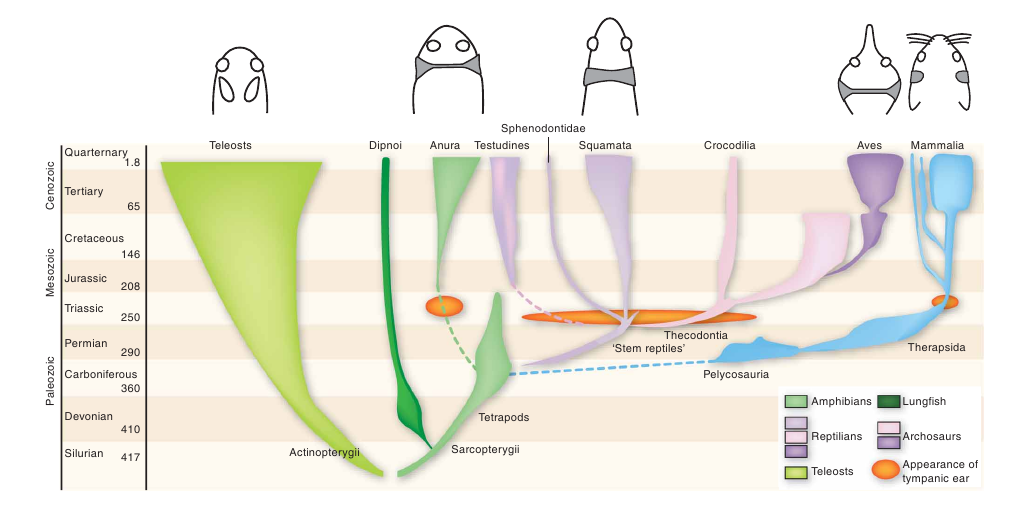
\includegraphics[width=1.0\linewidth]{Diagrams/vertebrateearevolution.png}
 \caption[Vertebrate Ear Evolution]{Figure due to Schnupp and Carr \cite{schnuppcarr}.}
 \label{vertebrateearevolution}
\end{figure}
  \chapter{The ICE Model}
Several terrestrial vertebrates, e.g. lizards, frogs, alligators and many birds, possess a hearing mechanism very different to
that of mammals: their tympanic membranes are coupled through large eustachian tubes and a large mouth cavity resulting in the influence of the vibrations of one tympanic membrane
on those of the other. This is illustrated in \ref{geckohead}. The typically small head sizes (compared to sound wavelength) of these animals result in
small phase differences (ITDs) and negligible amplitude difference (ILDs) between the ears. The coupling serves to enhance the ITDs and create ILDs
between the tympanal vibrations. These differences show directionality and serve as hearing cues for localization.

\begin{figure}[ht!]
 \centering
 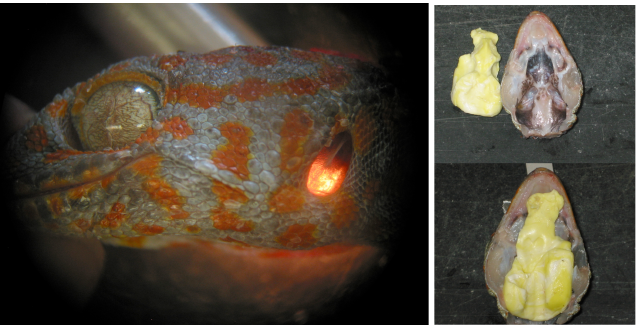
\includegraphics[width=.85\linewidth]{Diagrams/geckohead1.png}
 \caption[Illustration of a gecko's head]{Left: Picture of a Tokay gecko's head with the snout pointing to the left. The tympanic membrane is illuminated from behind by
 a light source on the other side of the head. The cartileginous extracolumella can be seen attached to the upper part of the membrane.
 Right: Cast imprint of the mouth cavity of the gecko with the snout pointing to the top. The figures illustrate the coupling of the tympani through the mouth cavity.
 Photographs courtesy of Jakob Christensen-Dalsgaard.}
  \label{geckohead}
\end{figure}

Proceeding from the earlier work done by Vossen in \cite{vossenthesis} and \cite{vossenjasa}, in this chapter we present a model for such a system of coupled ears with an emphasis on lizard hearing
- specifically the Tokay gecko and the common house gecko. Our goal is to demonstrate its main aspect of such a system - the coupling
of the eardrums through the mouth cavity. 
The main components of such a system are the mouth-cavity, the two tympani and the two \textit{extracolumella} (one on each tympanum). In general, the shape of the mouth-cavity is highly irregular and therefore
not conducive to an analytical treatment. Moreover, the system corresponds to a pair of coupled second-order PDE's with
moving boundaries. For this reason we will need to make further approximations in order to facilitate an
analytic solution.

In order to make the system more analytically tractable we will, as before, study a geometry in which a pair of rigidly clamped
linear elastic membranes are coupled through a cylindrical cavity. The cylindrical geometry allows an accurate calculation of the 
pressure distribution inside the cavity at both low and high frequencies. By accounting for the presence of the asymetrically attached
extracolumella, we will also explain the complex vibration patterns of the membrane. At the end of this chapter, we will
have the expressions that describe the steady-state vibrations of both eardrums as a function pressure amplitude, direction and frequency.

\section{Description of the Model}\label{description}
Before heading to a quantitative analysis of the ICE model, we will first need to list its basic components. 
and justify their properties based on a realistic mouth cavity. 

In Sec. \ref{subsecinnercavity}, we will describe the cylindrical model for the mouth cavity and state the reasons
for our choice of the geometry and the dimensions used. We will then proceed to describe the middle
ear system and its main components of interest, the \textit{extracolumella} and the \textit{tympani}
in Sec. \ref{middleear}. Finally, in Sec. \ref{soundinput} we will analyse the dependence of the acoustic input to both
eardrums on the direction of the sound source, head size and shape. 
\subsection{Mouth Cavity}\label{subsecinnercavity}
In the earlier treatment of the ICE model, the mouth canal is modelled as a simple cylinder closed at 
both ends by rigidly clamped (baffled) circular membranes; these model the tympanic membranes. As shown 
by Vossen in \cite[p.~21]{vossenthesis} and \cite{vossenjasa}, the length of the cylinder was chosen to be equal to the interaural distance and the radius of the model tympanum is
determined from the typical area of the realistic tympanum. The advantage of using a cylindrical cavity model for the mouth cavity is that the pressure
distribution inside the cavity is easy to calculate. The pressure distribution inside the cavity becomes highly non-uniform 
with increasing frequency and a cylindrical cavity simplifies its calculation. 

On the other hand, in this description the small area of the tympani results in a cavity volume which 
is an order of magnitude smaller than that of the realistic mouth-cavity in the corresponding animal. In general, a smaller volume results in a stronger coupling - both in terms of an increased iTD and an increased
iLD. For this reason, the earlier model overestimates the iTDs and iLDs at
low and high frequencies respectively.

In order to get around this problem we make some slight modifications to the model. Essentially, we maintain the cylindrical shape of the internal 
cavity but require it to have a volume which is equal to that of the realistic cavity ($V_{cav}$). We also maintain the same tympanum size and interaural distance
and can therefore calculate the radius of the cylinder as,
\begin{equation}\label{cylinderradiusformula}
 a_{cyl}=\sqrt{\frac{V_{cav}}{\pi L}}
\end{equation}
\begin{figure}[ht!]
\begin{center}
\begin{subfigure}{1.0\textwidth}
 \centering
  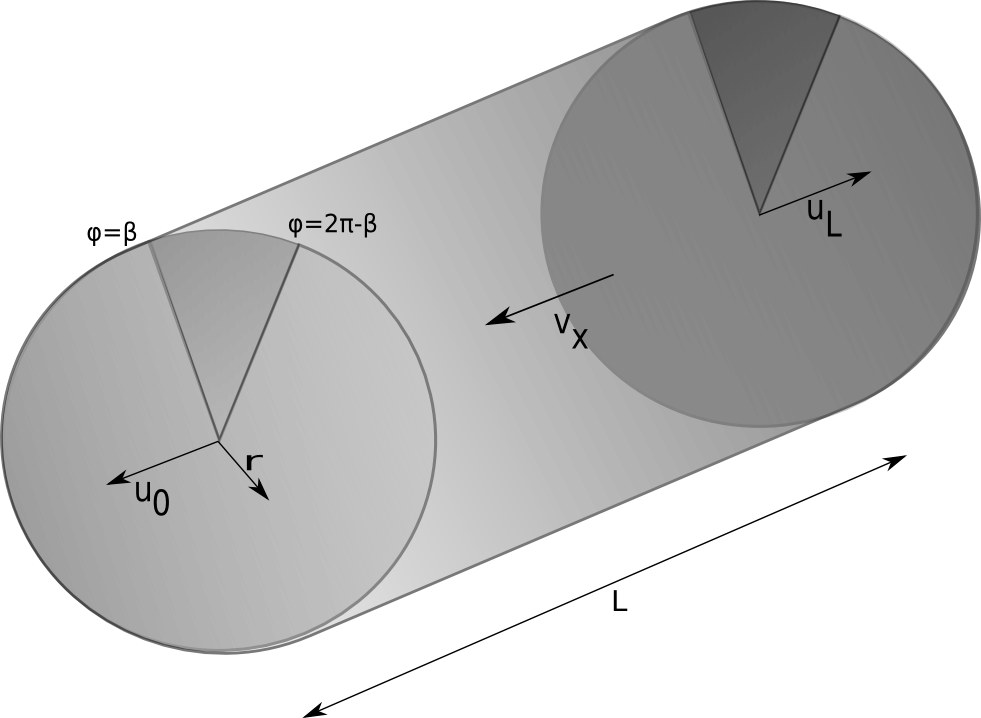
\includegraphics[width=.5\linewidth]{Diagrams/oldCylinder.png}
   \caption[Previous ICE Model Cylinder]{The previous geometric reprentation of the ICE model.}
  \label{oldICE}
\end{subfigure}

\begin{subfigure}{1.0\textwidth}
\centering
  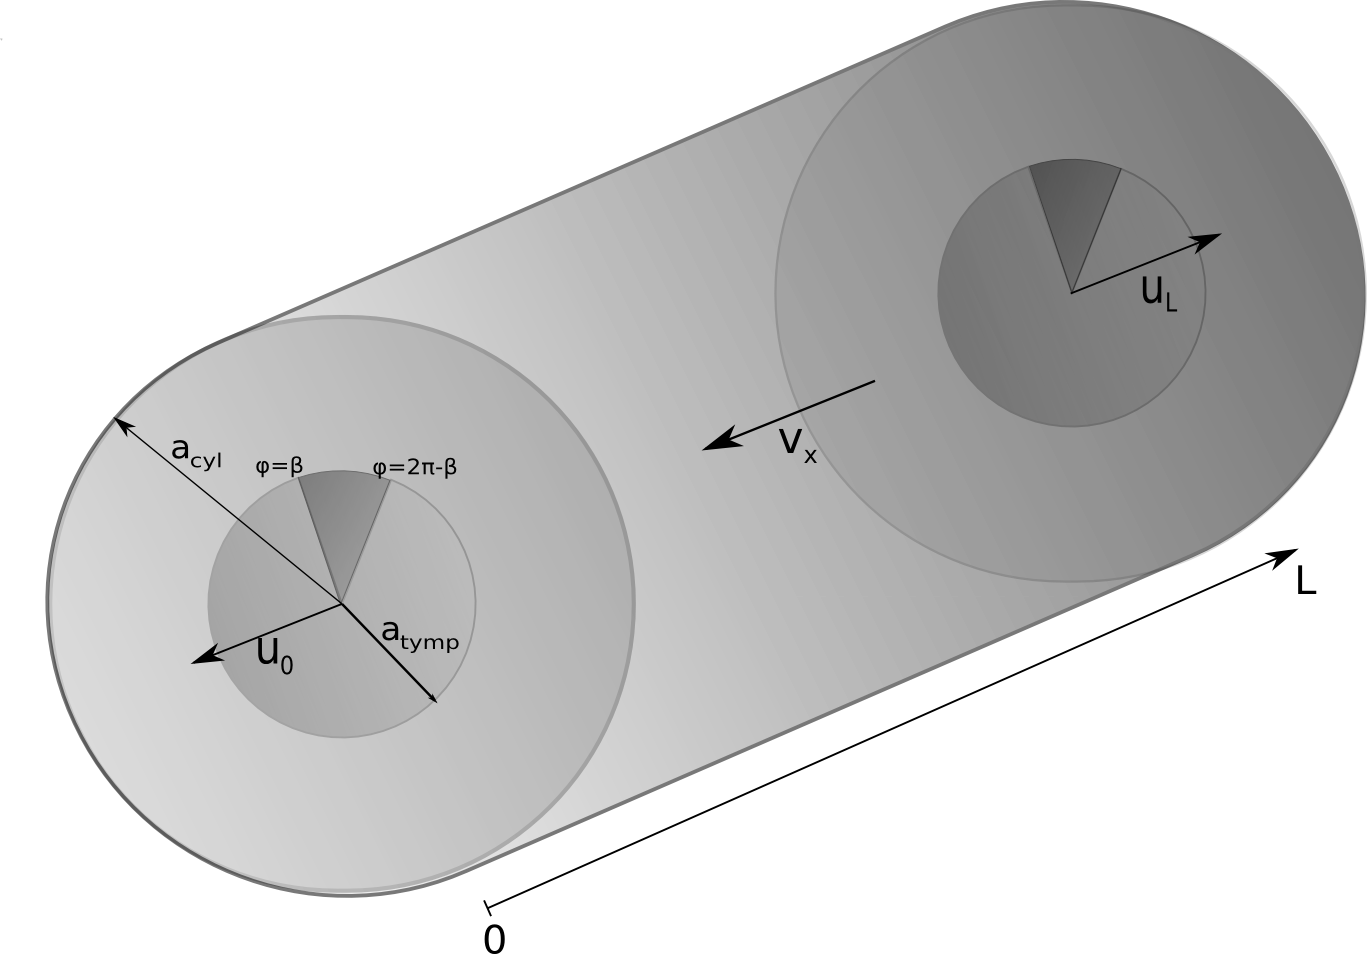
\includegraphics[width=.5\linewidth]{Diagrams/newCylinder.png}
  \caption[New ICE Model Cylinder]{The representation of the new model.}
  \label{newICE}
  \end{subfigure}
  \caption[Previous and current ICE model representations]{The bold arrows represent the direction conventions
  along the cylinder's axis. The new model is represented by a cylinder of radius $a_{cyl}$ and length $L$ closed
  at both ends by sectoral membrane of radius $a_{tymp}$.
  The darkly shaded region corresponds to the extracolumella (described in Sec. \ref{middleear}).}
\end{center}
\end{figure}
where $a_{cyl}$ is the cylinder radius and $L$ is the interaural distance. Simply put, the model consists of a cylindrical shell
of radius $a_{cyl}$ and length $L$ with circular holes on either side with the radius of the tympanic membrane, $a_{tymp}$. These
holes are in turn closed by rigidly clamped membranes which will be described in the next section. The previous and current geometric representations
of our model are shown in figures \ref{oldICE} and \ref{newICE}. The darkly shaded circular surfaces in fig. \ref{newICE} at ends $0$ and $L$ correspond to the two
eardrums.

We will be working with the cylindrical polar coordinates, $(r,\phi,x)$. The direction
along the cylindrical axis is denoted by $x$ and $(r,\phi)$ are the polar coordinates of the plane perpendular to the $x$-direction. 
Directions outward from the cylinder are taken as positive (in $x$) and those inward are taken as negative.
\subsection{Middle Ear System}\label{middleear}
The main components of the middle-ear of lizards are the two eardrums, the columella and the two cartileginous extracolumella.  
The tympanic membrane or the eardrum is a thin membrane that separates the outer ear and the
middle ear and vibrates in response to external sound waves.  Unlike humans, lizards 
possess only a single middle ear bone, the \textit{columella},
that is connected to both eardrums by means of a cartileginous element, the \textit{extracolumella}.

The membrane-extracolumella-columella system functions
as a second-order lever where the membrane - driven by the internal and external pressures - causes a displacement
of the extension of the extracolumella (known as the inferior process). This motion is in turn transmitted 
via the columella and columellar footplate to the inner ear (cochlea). The inner-ear translates this motion into
electrochemical impulses which will be passed on to the brain via the auditory nerve. The columella-extracolumella system effectively
transmits the mechanical vibrations from the eardrums to the inner ear. 
In the human middle-ear, the same function is
performed by the bones \textit{malleus, incus} and \textit{stapes}, which are collectively known
as the ossicles. 

For low frequencies (below $4$kHz), the extracolumella (or more accurately, the inferior process of the extracolumella)
moves as a completely stiff bar. It was shown by Manley \cite{manleygecko2} that the extracolumella begins to flex at higher frequencies - 
this is illustrated in fig. \ref{extracolumellaflection}. This is partly responsible for the poor high-frequency response of gecko middle ears - 
a feature also observed in other non-mammalian verterbates. The reason for this is that, due to the flection some energy is lost and
not transferred to the columella.

\begin{figure}[ht]
 \centering
 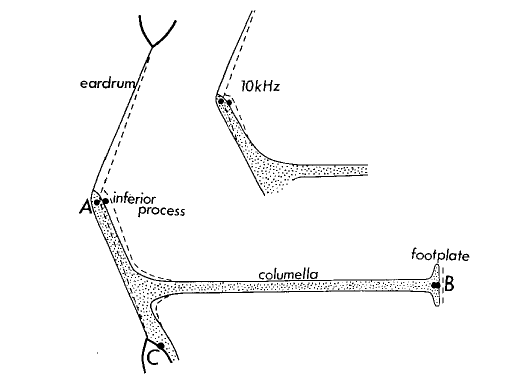
\includegraphics[width=.7\linewidth]{Diagrams/manleyextracolumellaflection.png}
 \caption[Extracolumella Flection]{Operation of the middle ear lever in geckos reproduced from \cite{manleygecko2}. The inferior process of the extracolumella (A-C) 
 hinges at point C at low frequencies. Also shown is the flection of the inferior process of the extracolumella.}
 \label{extracolumellaflection}
\end{figure}

\subsubsection{Tympanic Membrane}
The extracolumella applies a significant 
mechanical load on the tympanum and thereby precludes its treatment as a freely vibrating membrane. 
Furthermore, the contact surface of the malleus on the human eardrum is more or less symmetric whereas the 
extracolumella is attached asymetrically. This has important physical consequences - especially in the 
observed vibration patterns of the membrane.

In the previous treatment of the ICE model, the tympanum was modelled as a clamped circular membrane with assymetrically
attached sectoral load between $-\beta<\phi<\beta$ (\cite{vossenjasa}). This manifests itself as an additional
boundary condition at $\phi=\beta$ and $\phi=-\beta$ which has to satisfied via a numerical approximation. While
this method has the advantage of being able to accurately reproduce the complex vibration patterns of the eardrum, 
it does not lend itself well to an analytical treatment of the coupled system.

In our study, we will follow a slightly different path. The tympanic membrane will be modelled as a 
rigidly clamped sectoral membrane. This means that in addition to the radial boundary at $a_{tymp}$,
we have a new set of boundaries at $\phi=\beta$ and $\phi=2\pi-\beta$ where the membrane vibration is set to zero. This is illustrated in \ref{tympanummodel}.
The membrane material will be assumed to be linear-elastic. As before, the equations describing the vibrations of the membrane will 
consequently be linear $2^{nd}$-order PDE's.
\begin{figure}[ht]
 \centering
 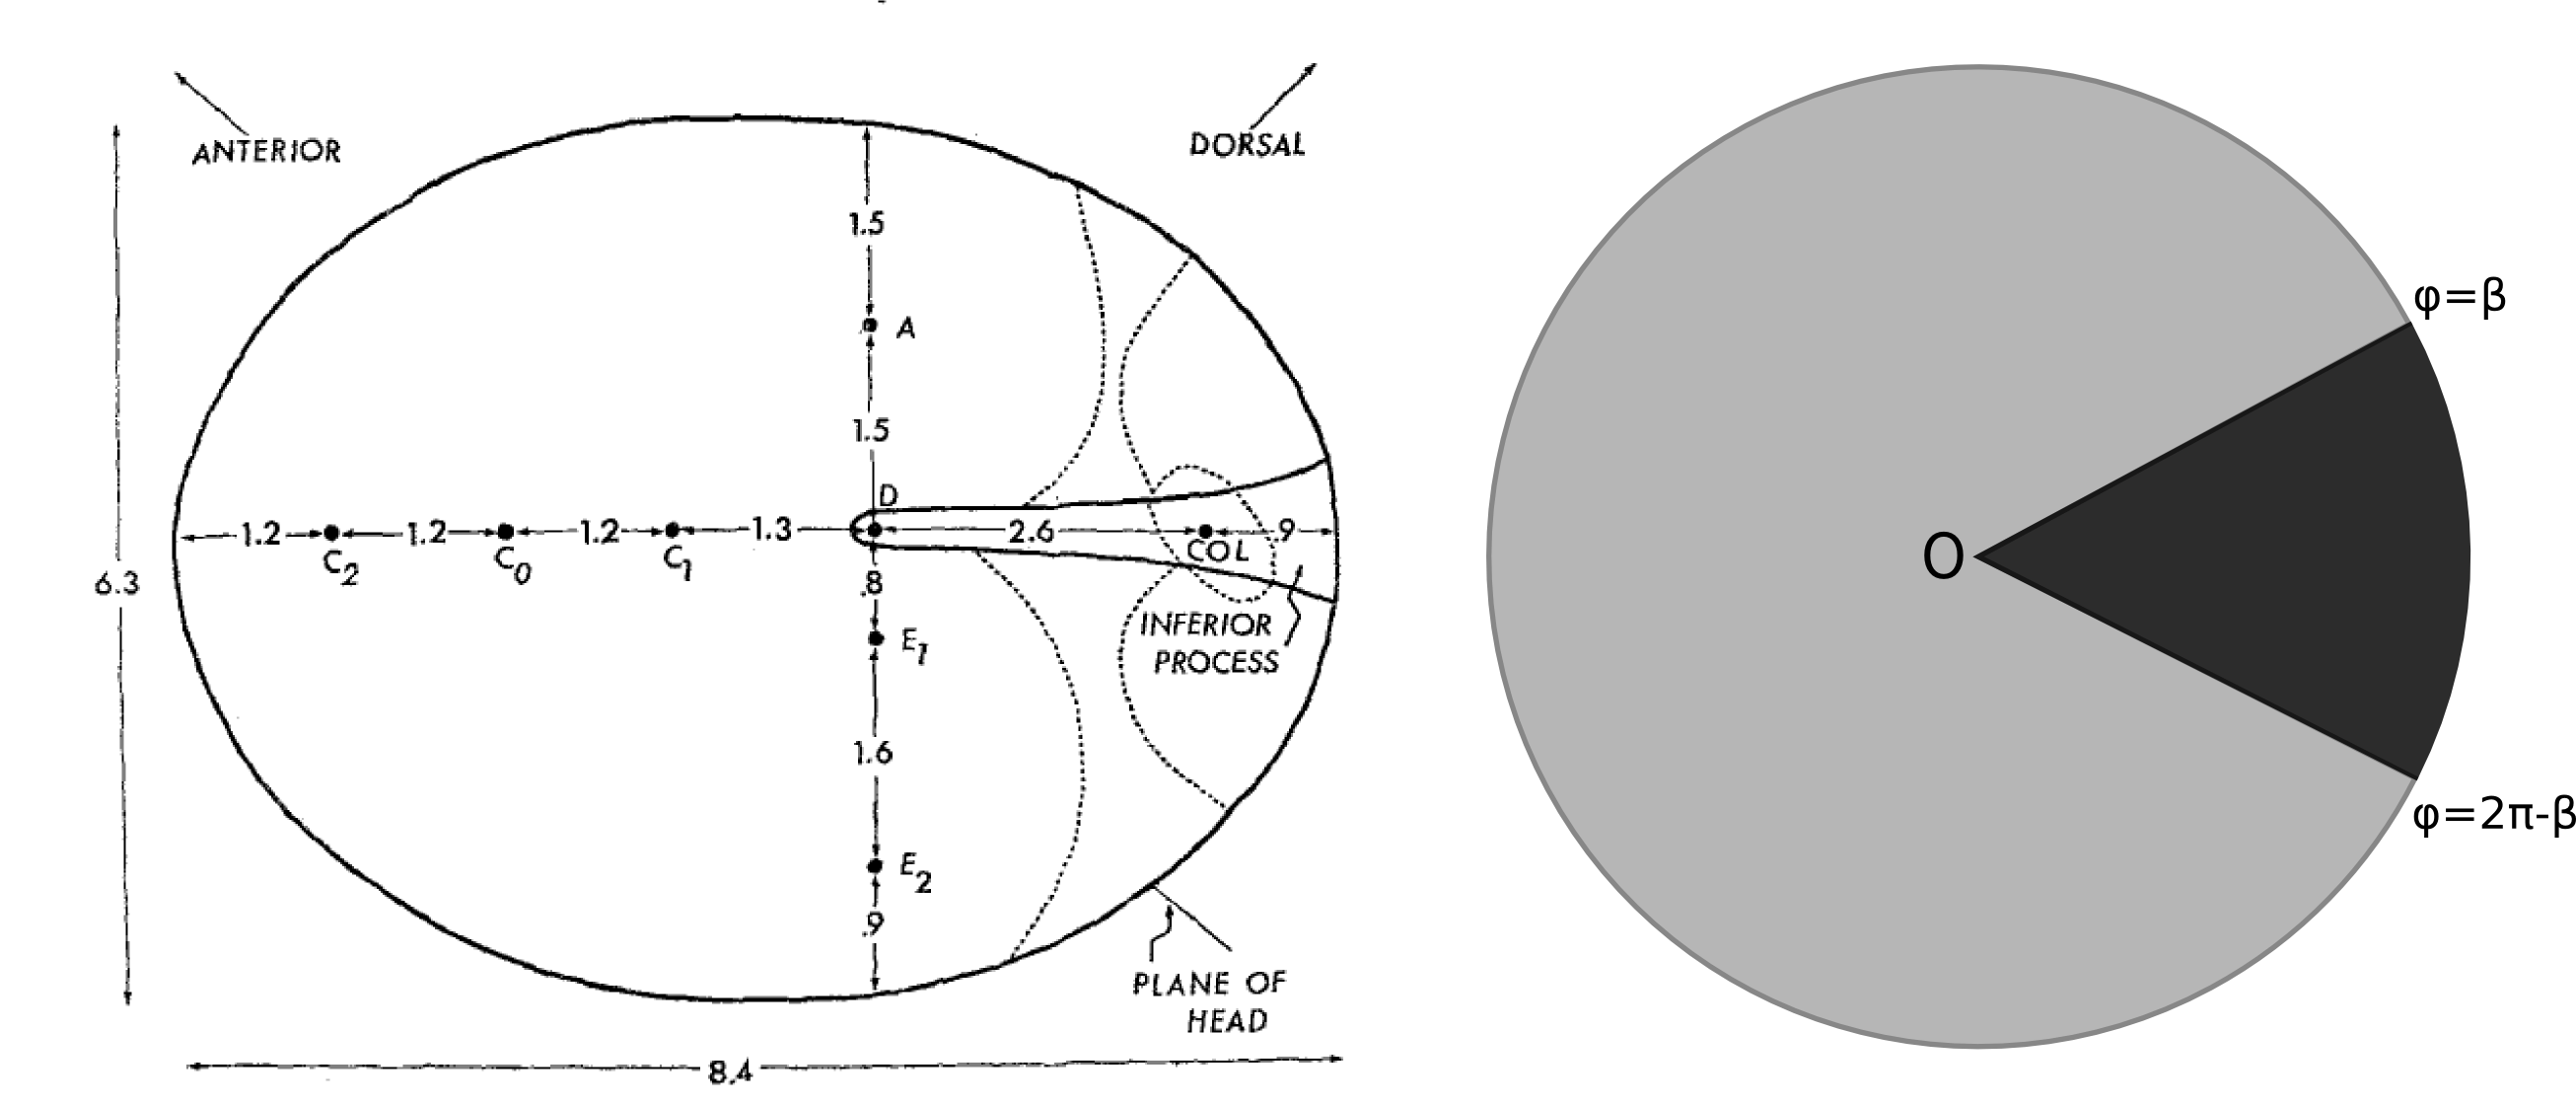
\includegraphics[width=.9\linewidth]{Diagrams/extracolumella2.png}
 \caption[Tympanic membrane model]{Left: Sketch of the eardrum of a Tokay gecko as seen from the outside taken from Manley, \cite{manleygecko1}. ``COL'' is
 the approximate position opposite the extracolumella insertion. The dots indicate the positions for measurements and will be discussed briefly in the
 next chapter. Dimensions
 in millimeters. Right: Our model for the loaded tympanic membrane. The lightly shaded region is modelled as a linear elastic membrane whereas the darkly shaded region 
 ($\beta<\phi<2\pi-\beta$) represents the contact surface of the extracolumella and the membrane. $\beta$ corresponds to the breadth of the extracolumella and is estimated from anatomical data.}
 \label{tympanummodel}
\end{figure}

At this point we should note that we have effectively set the mass of the extracolumella to infinity. Thereby, its motion has been neglected altogether. While this may seem counterintuitive at first, 
we will later see that this assumption, while simplifying the problem analytically,  has little effect on the physical phenomenon of interest, viz. the coupling between
the eardrums and the amplification of hearing cues. This will be discussed in-depth in Chapter \ref{modelanalysis}.

\subsection{Head Model and External Sound Input}\label{soundinput}
In realistic environments the acoustic fields experienced by animals are often very complex.
In addition to sound waves radiated directly from one or more sources in general, they also involve
waves reflected from objects in their immediate neighbourhood. Higher animals such as humans
possess the neural power to carry out the sophisticated signal processing needed to derive useful
information from these signals. Simpler animals like geckos respond to simpler cues - usually
the direct field from the nearest or strongest source.

We can therefore model our incoming wave as the simple case of an incident plane wave of a 
certain frequency. This input is specified in terms of its intensity, frequency and direction.
Such a stimulus can be generated in an anechoic chamber from loudspeakers which are placed at
a distance from the animal that is large compared to the animal's size and the wavelength
of the sound involved. Such experimental-setups are more thoroughly described by 
Christensen-Dalsgaard and Manley (\cite{dalsgaardmanley1}, \cite{dalsgaardmanley2}) and 
Christensen-Dalsgaard, Tang and Carr (\cite{dalsgaardtangcarr}).

The amplitude of the sound pressure incident on both ears can be taken as uniform in over 
the surface of the membrane. The spatial variation can be safely neglected because the
typical eardrum is less than $5$mm in diameter whereas the smallest sound wavelengths
in the hearing range of the larger lizards (eg. Tokay gecko) is around $70$mm ($4000$ Hz) 
and is around $50$mm ($7000$ Hz) for the smaller lizards (eg. Hemidactylus). In other
experiments, a similar stimulus has also been provided by means of a headphone sealed
to the ear (\cite{koepplcarr1}).

% In measuring the sound input, the important factors to be taken into account are
% \begin{itemize}
%  \item The separation of the ears and,
%  \item The overall head size
% \end{itemize}
In general a the sound on the other side of the head will differ in phase as well as amplitude. This is a result of the diffraction of 
sound around the head and body of the animal. The exact variation depends on the size of the animal and the frequency of the
incident wave. Due to the typically small head size of geckos, the amplitude variation 
(known as shadowing) is neglible (\cite{michelsenlarsen}). The phase difference, although small compared to those in larger animals, 
cannot be neglected. We can therefore consider the sound wave with angular frequency $\omega$ to have a constant (pressure) amplitude $p$
on the head.

In the earlier ICE model, the effect of diffraction on the phase difference was neglected as well. The phase difference
is found directly from the phase difference $\Delta$ as shown in fig. \ref{fig:oldheadmodel}.
As a result, the sound pressure inputs at both ears is given by,
\begin{equation}\label{oldsoundinput}
p_0=pe^{j\omega t} e^{-\Delta/2},\qquad p_L=pe^{j\omega t} e^{\Delta/2},\qquad \Delta=kL\sin\theta.
\end{equation}
We note that in defining the input in this way, we've emphasized the symmetry of the system.
The ear closer to the sound source is referred to as the \textit{ipsilateral} ear and
is denoted by a subscript $0$ and the one further away from the source is referred to as the \textit{contralateral} ear and is denoted by a subscript $L$. 
Subsequently, unless otherwise specified, the subscripts $0$ and $L$ will correspond to the ipsi- and contralateral ears respectively.
\begin{figure}[ht]
 %\centering
 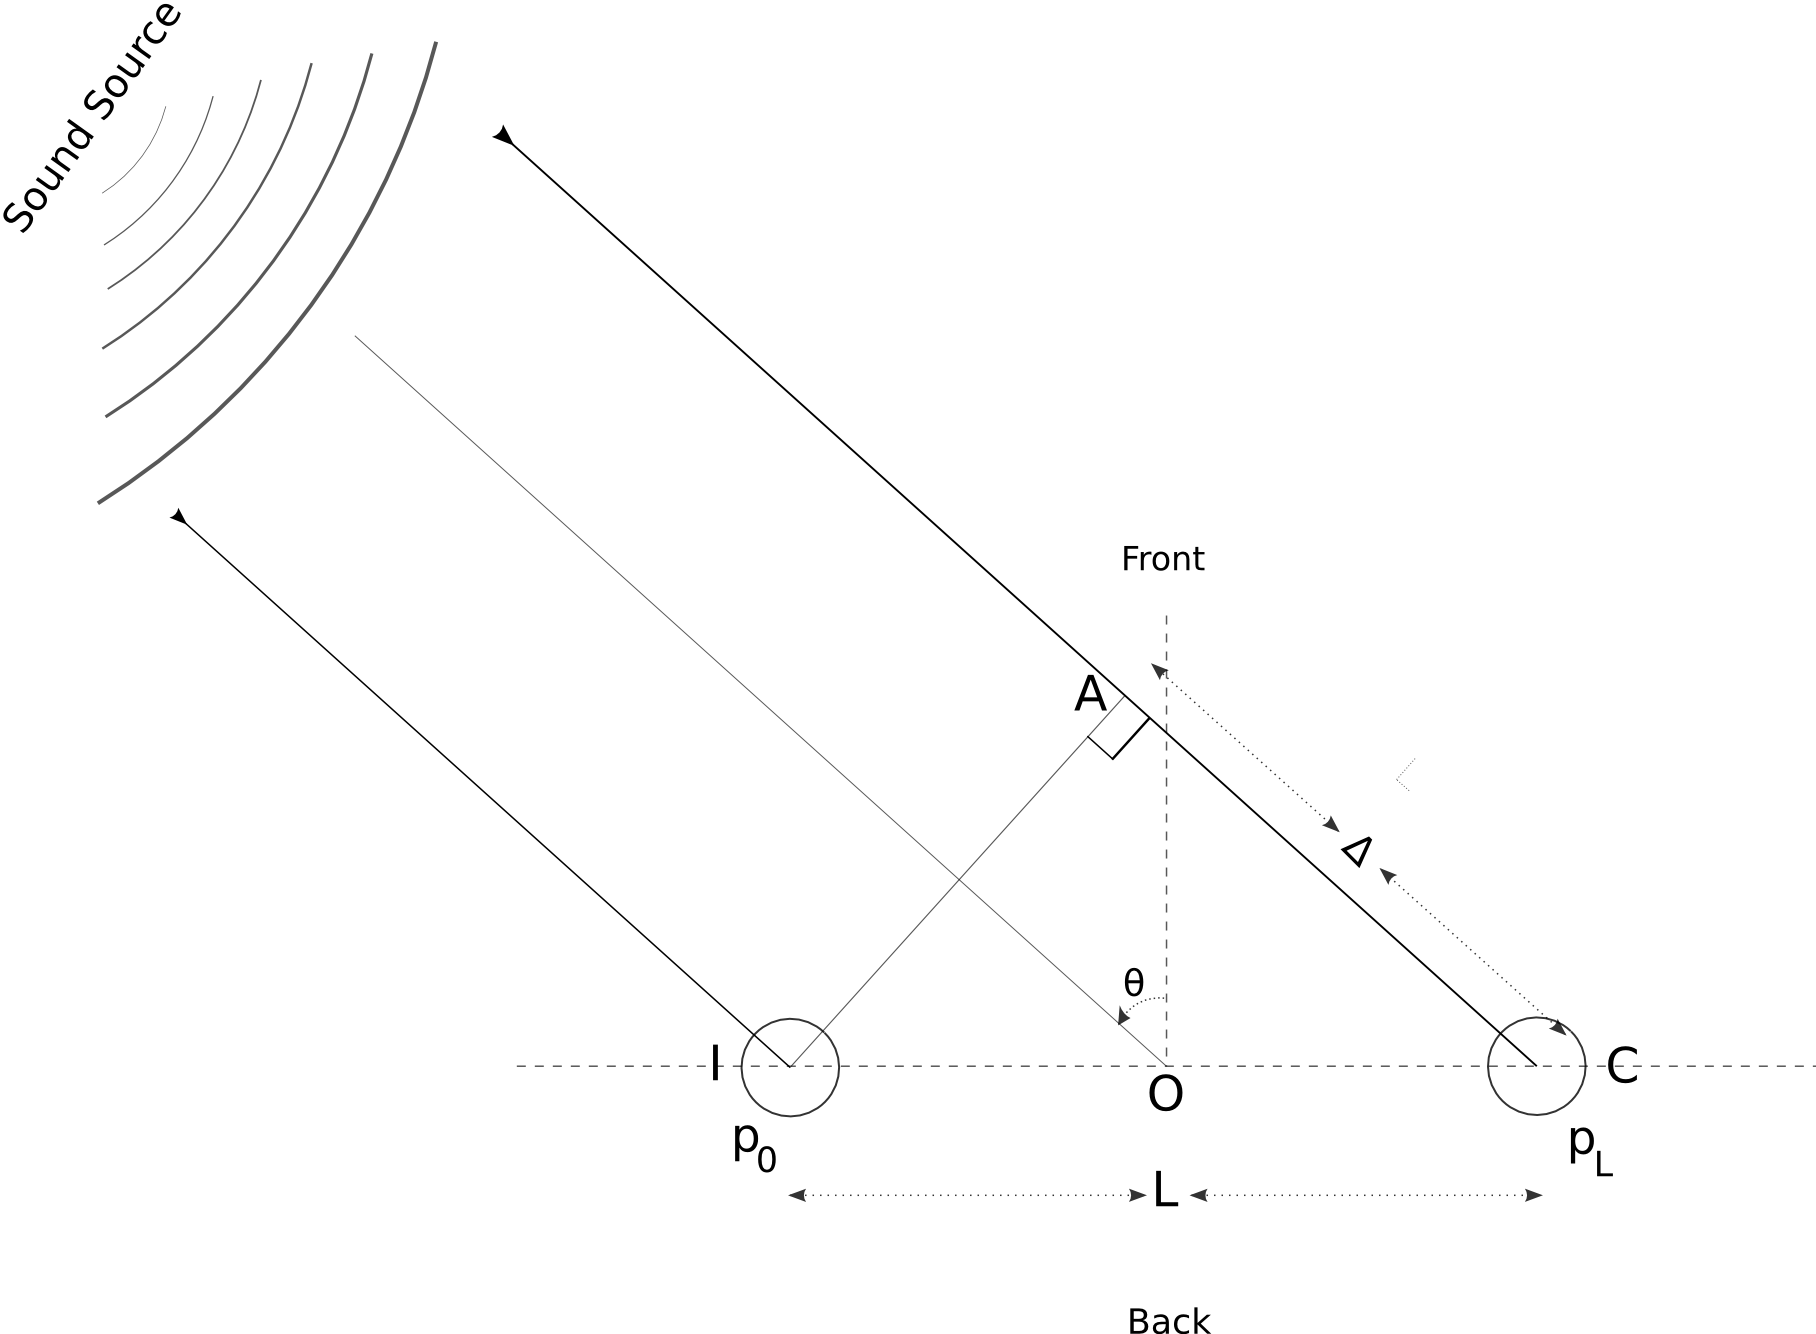
\includegraphics[width=.75\linewidth]{Diagrams/acousticheadmodelold.png}
 \caption[Previous acoustic head model for geckos]{The previous acoustic head model for geckos. The extra distance travelled by the sound wave to reach the contralateral ear 
 is denoted by $\Delta$.}
 \label{fig:oldheadmodel}
\end{figure}
We have also chosen a coordinate
system relative to the \textit{median-sagittal} plane or the head midline of the animal and $\theta$ gives the angle of incidence of this
sound wave relative to this plane. For more complex auditory systems we would require two angles $(\theta, \phi)$ to describe
the three-dimensional system but in our analysis this is unnecessary. For the animals we are concerned with, i.e. geckos, the natural
predators and prey are usually present on the same plane as the animal and our assumption is therefore reasonable.

\begin{figure}[ht]
 %\centering
 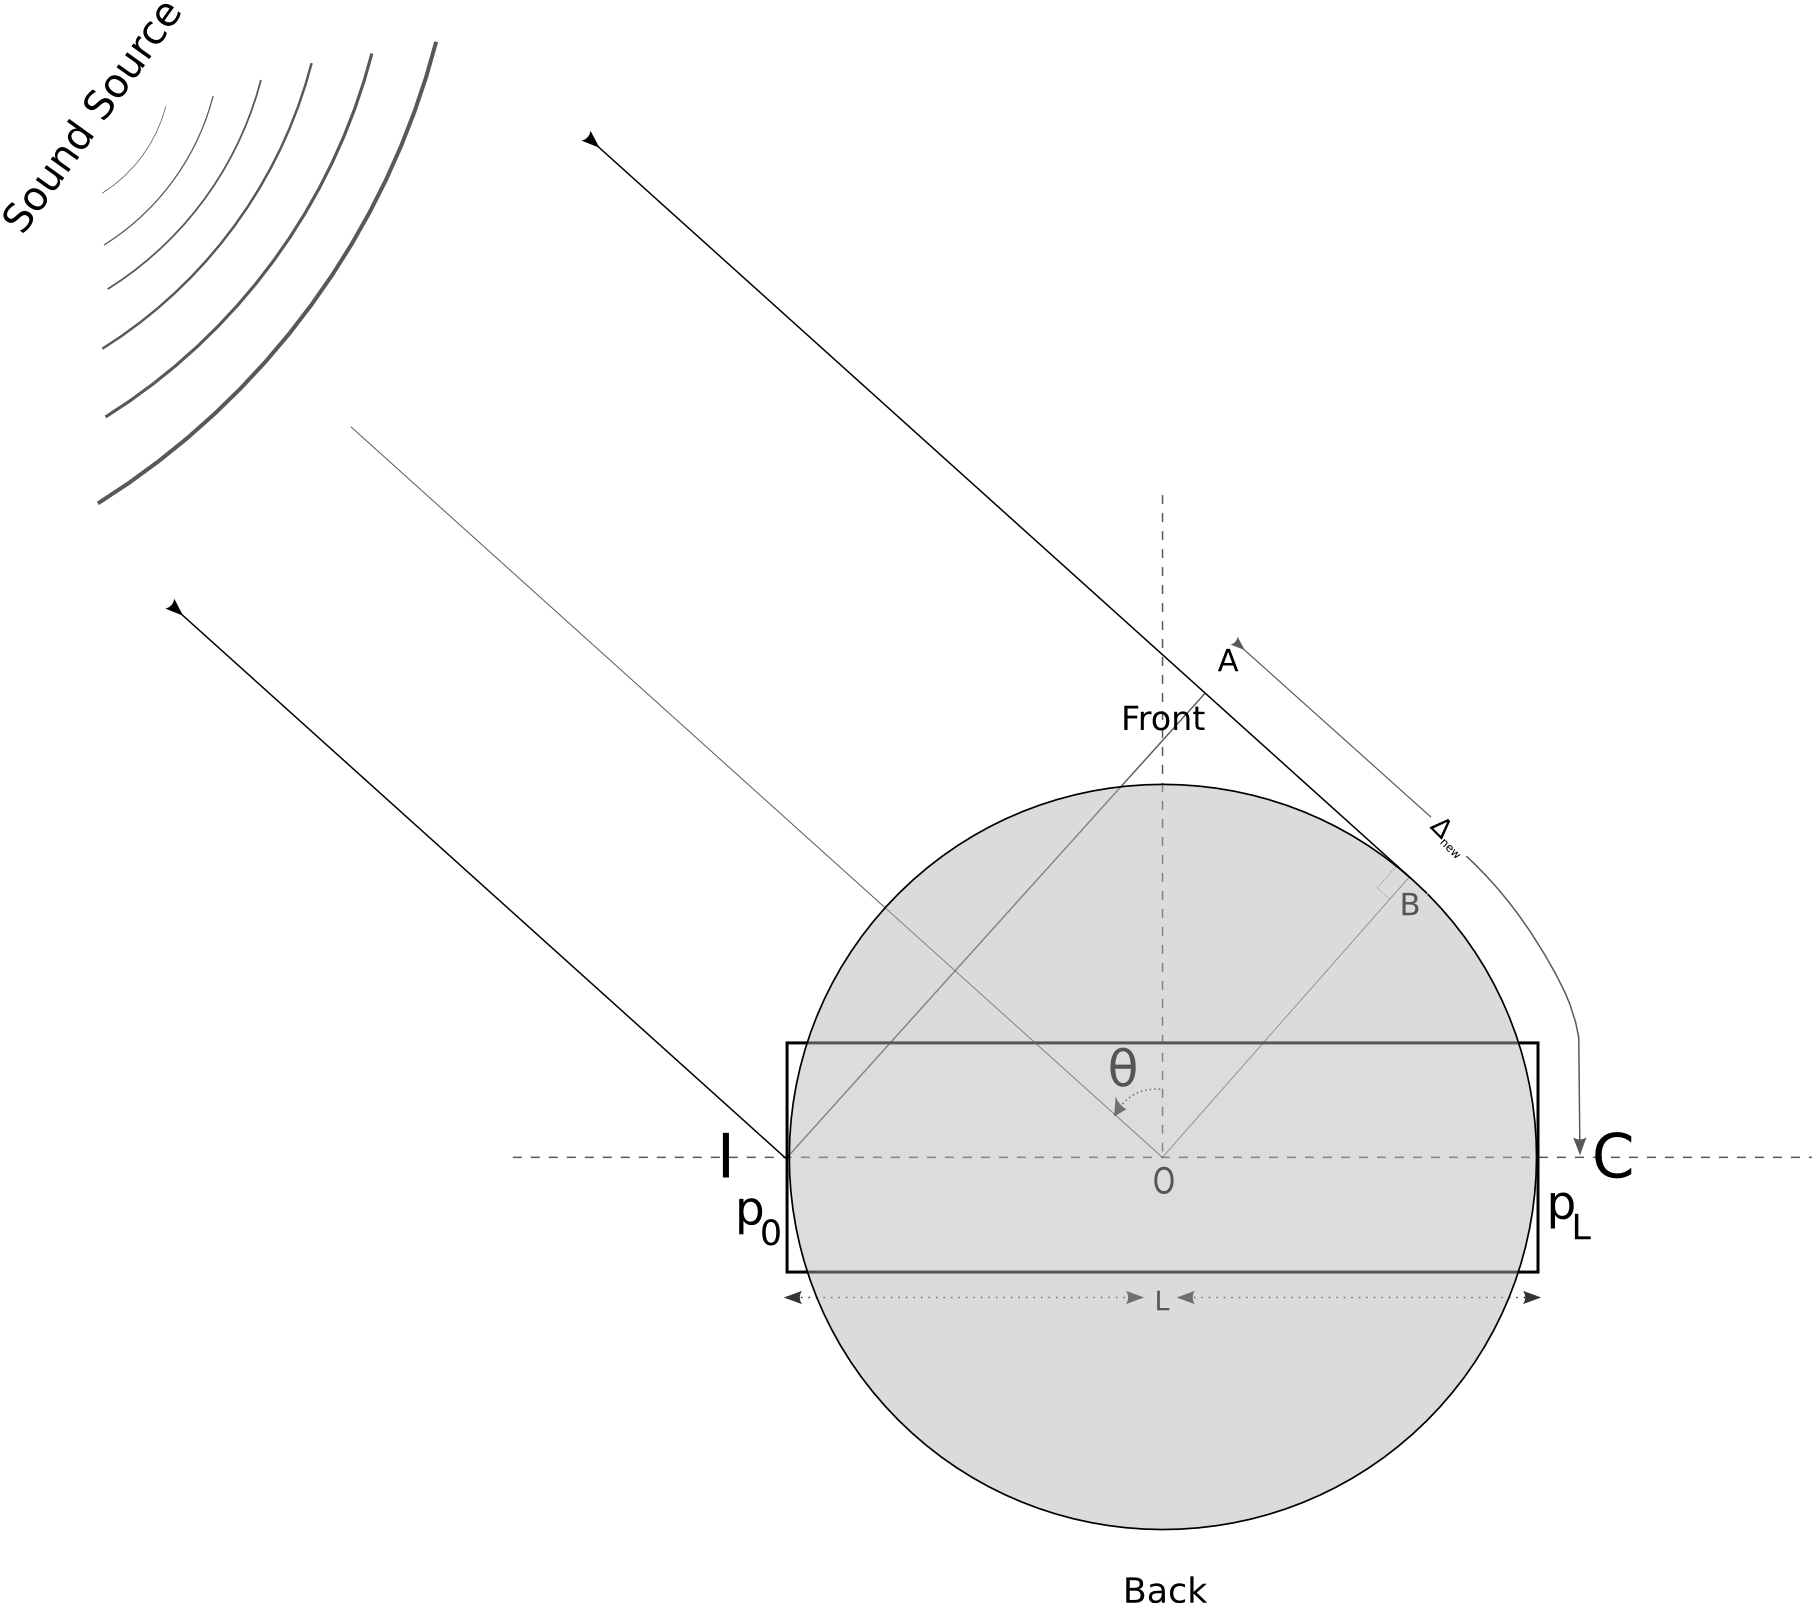
\includegraphics[width=.75\linewidth]{Diagrams/acousticheadmodel2.png}
 \caption[New acoustic head model for geckos]{The acoustic head model for geckos. The rectangular outline 
 is the internal cavity. As before, the extra distance travelled by the sound wave to reach the contralateral ear is given by 
 $\Delta$. In this case, however, we have accounted for the influence of diffraction around the head on the phase difference between the inputs
 to both ears.}
 \label{newheadmodel}
\end{figure}
In our model we model the head as a sphere with a diameter equal to the interaural separation. As a result the sound has to travel around the 
head in order to reach the contralateral ear resulting in a longer path. The frequency domain solution for the diffraction of sound around a
sphere was obtained by Lord Rayleigh at the end of the $19^{\mbox{th}}$ century (\cite{rayleigh1},\cite{rayleigh2}). The expressions 
are greatly simplified at low frequencies and the phase difference is simply increased by by a factor of $1.5$. The new model is illustrated in Fig. \ref{newheadmodel}.
Therefore, the form of the input remains the same as in \eqref{oldsoundinput} expect for a new phase difference  $\Delta_{new}=1.5\Delta$.

\section{Derivation of the Model}
We will now use the previously described physical model to derive the main expressions of interest in the ICE model - the membrane
vibration profiles, the ipsi- and contraleteral filters and the cavity pressure distribution. We will thus find an expression for the pressure 
distribution in the cylindrical cavity and for the membrane vibrations subject to an external stimulus. After applying the 
appropriate boundary conditions to relate the membrane vibrations to the internal pressure, we will find the expression for the membrane
vibrations as a function of direction and frequency.

We will start in Sec. \ref{internalcavity} by finding a general solution to a $2^{nd}$-order PDE - the $3$D wave
equation - that describes the pressure distribution inside the cylindrical cavity. In this section we will introduce the
main boundary condition the pressure will be subject to - the ``no-penetration'' boundary condition. This is a physical requirement that results from the fact that the air
inside the cavity does not penetrate a solid boundary.

In Sec. \ref{membranevibrations} we will solve for the vibrations of the tympanic membranes. As an example, we
will find an expression for the free and periodically driven vibrations of a circular membrane. Using the methods
developed in this section, we will solve for the vibrations of a sectoral membrane - which, as we have already discussed,
models the loaded tympanum. The final expression will correspond to the steady-state vibrations of a linear elastic
membrane. As we neglect the transient response of the membrane, we will also discuss the circumstances under which this
is justified.

\noindent
\begin{minipage}{\linewidth}
\renewcommand{\arraystretch}{1.1}
%\caption{Parameters and Functions used in the ICE Model} \label{parametertable} 
\centering
\captionof{table}{Functions and Parameters used in the ICE Model} \label{parametertable} 
\begin{tabular}{c p{12 cm}}
\hline
$\theta$ & Direction of the sound source with respect to the head midline.\\
$\omega$ & Angular frequency of the incoming sound wave.\\
$k$ & Wavenumber $k=\omega/c$ with $c=343$m/s being the speed of sound.\\
$p$ & Pressure amplitude of the incoming sound wave.\\
$\Delta$ & Phase difference between the sound wave reaching the contra- and ipsilateral ear.\\
$p_{0/L}$ & Sound pressure on the ipsi- ($x=0$) and contralateral ($x=L$) ears respectively.\\
%& \\
$(x,r,\phi)$ & Cylindrical polar coordinates with $x$ being the axial direction.\\
$L$ & Interaural separation and length of cylinder.\\
$a_{cyl}$ & Radius of cylinder.\\
$a_{tymp}$ & Radius of tympanum.\\
$\beta<\phi<2\pi-\beta$ & Extent of the vibrating part of the membrane. The rest of the circle corresponds to
the extracolumellar footplate.\\
$V_0$ & Volume of the cavity.\\
\hline
\end {tabular}\par
\bigskip
\end{minipage}
In Sec. \ref{coupledmembranes} we will conclude by using our knowledge to solve for the vibration of the fully coupled
system. In this section we will  proceed by applying the velocity boundary condition at either end of the cylinder. In
order to help with our analysis, we will present a simplification scheme for this boundary condition. We will end this section
by defining the ipsi- and contralateral filters. The final expressions that give us the vibrations 
of the tympanic membranes as a function of the external pressure with the influence of the internal cavity encoded in the ipsi- and contralateral filters. 
We have listed the main parameters and functions used in our analysis (including the geometry parameters) in Tables \ref{parametertable}
and \ref{functiontable}.
\begin{minipage}{\linewidth}
\renewcommand{\arraystretch}{1.1}
%\caption{Parameters and Functions used in the ICE Model} \label{parametertable} 
\centering
\captionof{table}{Functions and Parameters used in the ICE Model contd.} \label{functiontable} 
\begin{tabular}{c p{13 cm}}
\hline
$J_q$ & Order $q$ Bessel function of the first kind.\\
$\mu_{qs},\nu_{qs}$ & Respectively - $s^{th}$ zero and $s^{th}$ extremum of the above Bessel function.\\
$f_{qs}(x,r,\phi)$ & Orthogonal modes for the pressure distribution inside the mouth cavity.\\
$\zeta_{qs}$ & Wavenumber of the above modes in the $x$-direction.\\
$p(x,r,\phi;t)$ & Pressure distribution inside the mouth cavity.\\
$v_x(x,r,\phi;t)$ & Velocity function inside the mouth cavity.\\
&\\
$u_{mn}(r,\phi;t)$ & Eigenmodes of the membrane displacement function.\\
$\omega_{mn}$ & Eigenfrequency of the above eigenmodes.\\
$Q$ & Quality factor of the membrane.\\
$\Psi(r,\phi;t)$ & Driving pressure on the membrane.\\
$u_{0/L}(r,\phi;t)$ & Membrane displacement function.\\
$S^{0/L}(t)$ & Total membrane displacement.\\
&\\
$G_{ipsi}(r,\phi)$ & Ipsilateral filter.\\
$G_{contra}(r,\phi)$ & Contralateral filter.\\
\hline
\end {tabular}\par
\bigskip
\end{minipage}
\subsection{Internal Cavity}\label{internalcavity}
We assume that the air inside the cavity obeys linear acoustics (cf. acoustic textbooks such as \cite[p.~313]{rschevkinsound} and \cite[p.~247]{temkinelements} ). 
This means that the air moves due to pressure $p(x,r,\phi;t)$ whose distribution inside the cavity
is given by the $3$D acoustic wave-equation in cylindrical polar coordinates,	
\begin{equation}\label{pressurewaveeqn}
 \frac{1}{c^2}\frac{\partial^2 p(x,r,\phi,t)}{\partial t^2}=\frac{1}{r}\frac{\partial}{\partial r}\left(r\frac{\partial p(x,r,\phi,t)}{\partial r}\right)
 +\frac{1}{r^2}\frac{\partial p(x,r,\phi,t)}{\partial \phi^2}+\frac{\partial p(x,r,\phi,t)}{\partial x^2}
\end{equation}
where $c$ is the sound propagation velocity. The complete solution must take into account the boundary conditions at and within the cavity walls and the
ones at the air-membrane interface. We also note that the above equation implies that the animal's mouth is closed, which is typical for a waiting
animal. In order to solve \eqref{pressurewaveeqn} for a particular frequency $f$ (angular frequency $\omega=2\pi f$), we use the following
separation ansatz
\begin{equation}\label{pseparationansatz}
  p(x,r,\phi,t)=f(x)g(r)h(\phi)e^{j\omega t}
\end{equation}
which after substitution into the acoustic wave-equation leads to,
\begin{equation}\label{pseparationansatz2}
\begin{split}
 k^2f(x)g(r)h(\phi)+&f(x)h(\phi)\left[\frac{\partial^2 g(r)}{\partial r^2} + \frac{1}{r}\frac{\partial g(r)}{\partial r}\right] \\
 &+f(x)g(r)\frac{1}{r^2}\frac{\partial h(\phi)}{\partial \phi}+\frac{\partial^2 f(x)}{\partial x^2}=0
\end{split}
\end{equation}
with $k:=\omega/c$. This results in the following set of separated ODE's,
\begin{align}
 \frac{d^2 f(x)}{dx^2}+\zeta^2f(x)&=0\\
 \frac{d^2 h(\phi)}{d\phi^2}+q^2h(\phi	)&=0\\
 \frac{\partial^2 g(r)}{\partial r^2} + \frac{1}{r}\frac{\partial g(r)}{\partial r}+\left[(\displaystyle\underbrace{k^2-\zeta^2}_{=:\nu^2})-\frac{q^2}{r^2}\right]g(r)&=0\label{besselequation1}
\end{align}
with separation constants $q$ and $\zeta$. The last equation is the Bessel differential equation \cite[p.~313]{copsonbessel} and its general solution is given by,
\begin{equation}
 g(r)=C_{qs}J_q(\nu r)+D_{qs}Y_q(\nu r).
\end{equation}
$J_q$ and $Y_q$ are the order-$q$ Bessel functions of the first and second kind respectively. The Bessel function of the second kind can be ignored as it diverges at $r=0$.
The solutions to the separated equations are therefore given by,
\begin{equation}
 f(x)=e^{\pm \zeta x},\ h(\phi)=e^{\pm j\phi},\text{and}\ g(r)=J_q(\nu r)
\end{equation}
with a specific solution to \eqref{pressurewaveeqn} given by,
\begin{equation}\label{specificpressure1}
 p(x,r,\phi;t)=\left[(A^+e^{jq\phi}+A^-e^{-jq\phi})e^{j\zeta x}+(B^+e^{jq\phi}+B^-e^{-jq\phi})e^{-j\zeta x}\right]J_q(\nu r)e^{j\omega t}.
\end{equation}
The coefficients $A^\pm$, $B^\pm$, $q$, $\zeta$ and $\nu$ will be subsequently determined by the boundary conditions. 
Before we move on to the boundary conditions we should note that in general, the time component of the pressure also has a \textit{backward-moving} component, i.e. $e^{-j\omega t}$. 
By making the ansatz in \eqref{pseparationansatz}, we have implicitly made use of the fact that the form of the input as given in \eqref{oldsoundinput} constrains the pressure to only have a \textit{forward-moving} component, i.e. $e^{j\omega t}$.  
\subsubsection{Pressure Boundary Conditions}\label{pressureboundaryconditions}
There are three sets of boundary conditions - 
\begin{itemize}
 \item Continuity and smoothness in $\phi$ which is equivalent to $h(0)=h(2\pi)$ and $h^\prime(0)=h^\prime(2\pi)$ where, $h^\prime=dh/d\phi$.
 \item Vanishing of the normal derivative at the cavity walls - $g^\prime(a_C)=0$ ($a_C$ is the radius of the cylinder).
 \item Equating the membrane velocity to the velocity function at the membrane boundaries (to be discussed in the next section).
\end{itemize}
The first set of requirements is obvious. This reduces \eqref{specificpressure1} to 
\begin{equation}\label{specificpressure2}
 p(x,r,\phi;t)=\left[Ae^{j\zeta x}+Be^{-j\zeta x}\right]\cos q\phi J_q(\nu r)e^{j\omega t}.
\end{equation}
With $q$ constrained to be an integer.

The second and third are a result of the so called ``no-penetration'' boundary-condition
of fluid-mechanics. It arises from the from the fact that the cavity wall is an impermeable boundary. This translates 
into the requirement that the normal velocity function should vanish (\cite[p.~111]{pozrikidisFluid}).
The velocity function ($\mathbf{v}$) is related to the pressure by, 
\begin{equation}\label{pressurevelocityrelation}
 -\rho\frac{\partial \mathbf{v}}{\partial t}=\nabla p
\end{equation}
At the cylindrical cavity wall, the normal velocity is in the radial direction.
Substituting the expression for pressure in \eqref{specificpressure1} in the above equation leads to
a Neumann boundary condition for the pressure,
\begin{align}\label{radialnopenetration}
 v_r=-\left.\frac{1}{j\rho\omega}\frac{\partial p(x,r,\phi;t)}{\partial r}\right\vert_{r=a_C}&=0\nonumber\\
    \Rightarrow\left.\frac{\partial J_q (\nu r)}{\partial r}\right\vert_{r=a_C}&=0
\end{align}
This constrains $\nu$ to a discrete set of values which correspond to the local minima and maxima
of $J_q$. We can therefore index $\nu$ by $q$ and $s=0,1,2,3,\ldots$ with $\nu_{qs}=z_{qs}/a_C$:
$z_{qs}$ being the $s^{th}$ extremum of the order-$q$ Bessel function of the first kind.
This results in a discrete set of modes that satisfy \eqref{pressurewaveeqn} which are given
by,
\begin{equation}\label{specificpressure3}
 p_{qs}(x,r,\phi;t)=\left[A_{qs}e^{j\zeta_{qs}x}+B_q{s}e^{-j\zeta_{qs}x}\right]f_{qs}(r,\phi)e^{j\omega t}
\end{equation}
where we have added the subscripts $q$ and $s$ to $\zeta$ and denoted the $(r,\phi)$ part of \eqref{specificpressure2}
by $f_{qs}(r,\phi)$. Effectively, the
modes are 3D waves propagating with wave numbers $\zeta_{qs}$ in the $x$-direction and $\nu_{qs}$ in the radial
direction. The first of these modes (corresponding to $q=0,s=0$) is of particular importance. Since the first
maximum of $J_0$ occurs at $r=0$, we have $\nu_{00}=0$. This leads to the first mode being a plane-wave which
is constant in $r$ and $\phi$ and only varies in $x$. 

A very useful property of the above modes is their orthgonality, i.e.
\begin{equation}\label{pressureorthogonality}
 \int_\Omega dVp_{q_1s_1}p_{q_2s_2}=0,\ if\ q_1\neq q_2\ or\ s_1\neq s_2
\end{equation}
the integral is over the volume	 of the cylinder. This is a consequence of the fact that for different $q$'s
the cosine parts of the modes are orthogonal whereas for a given $q$ the Bessel parts are orthogonal for
different $s$'s or expressed as an equation,
\begin{equation}\label{besselorthogonality}
 \int dS f_{q_1s_1}f_{q_2s_2}=0,\ q_1\neq q_2\ or\ s_1\neq s_2
\end{equation}
where $dS=rdrd\phi$ and the integral being taken over the disk of radius $a_C$.
We can therefore write the general solution to \eqref{pressurewaveeqn} as a linear combination of the orthogonal modes given in \eqref{specificpressure3},
\begin{equation}\label{pressuregeneral1}
 p(x,r,\phi;t)=\displaystyle\sum^\infty_{q=0}\displaystyle\sum^\infty_{s=0}\left(A_{qs}e^{j\zeta_{qs}x}+B_{qs}e^{-j\zeta_{qs}x}\right)f_{qs}(r,\phi)e^{j\omega t}
\end{equation}
The remaining coefficients, $A_{qs}$ and $B_{qs}$, will be determined by equating the velocity function to
the membrane velocity at both ends of the cylinder. To do so, we will first need to find an expression
for the membrane vibrations - as we will in the following section.

\subsection{Vibration of the Membrane}\label{membranevibrations}
As a preliminary exercise, we will first derive expressions for the free and force-driven
vibrations of a circular membrane. We will then use our results to move on to the sectoral membrane 
which corresponds to the tympanum loaded by the extracolumella. Thi corresponds to the approximating
the extracolumella to have infinite mass. 
\subsubsection{Circular Membrane}
The equation of motion for the vibration of a rigidly clamped circular membrane of radius $a_M$ solves for the membrane displacement $u$ at
a point $(r,\phi)$ with $r<a$ and $0<\phi<2\pi$. It is given by,
\begin{equation}\label{membraneequation1}
 \begin{split}
 -\frac{\partial^2 u(r,\phi;t)}{\partial t^2}-2\alpha\frac{\partial u(r,\phi;t)}{\partial t}+c^2_M \left[\frac{1}{r}\frac{\partial}{\partial r}\left(r\frac{\partial u(r,\phi,t)}{\partial r}\right)\right. +\frac{1}{r^2}&\left.\frac{\partial u(r,\phi,t)}{\partial \phi^2}\right]
 \\ &=\frac{1}{\rho_M d}\Psi(r,\phi;t)
 \end{split}
\end{equation}
subject to the boundary condition $u(r,\phi;t)|_{r=a_M}=0$.. We've defined the following membrane material properties,
\begin{itemize}
 \item $c_M$ - propagation speed of vibrations.
 \item $\alpha (>0)$ - the damping coefficient.
 \item $\rho_M$ - density.
 \item $d$ - thickness.
\end{itemize}
$\Psi(r,\phi;t)$ is the pressure on the membrane surface at $(r,\phi)$. In our discussion we are only concerned with periodic and uniform 
pressure acting on the membrane surface. As we have already stated in Sec. \ref{soundinput},  the small size of the membrane with respect to the sound wavelength,
justifies the spatial uniformity of our input.
\subsubsection*{Free Vibrations}
\noindent\textbf{Undamped Membrane}: We first determine the eigenmodes of an undamped circular membrane by solving \eqref{membraneequation1} for $\alpha=0,\ \Psi=0$
(the resultant equation is better known as the $2$D Helmholtz equation, cf. \cite[p.~187]{asmar2005partial}). Just as we did in \eqref{pseparationansatz},
we do this by making a separation ansatz ,
\begin{equation}\label{mseparationansatz}
 u(r,\phi;t)=f(r)g(\phi)h(t)
\end{equation}
This gives us the following set of equations
\begin{align}
 \frac{\partial^2 f(r)}{\partial r^2} + \frac{1}{r}\frac{\partial f(r)}{\partial r}+\left[\mu^2-\frac{m^2}{r^2}\right]f(r)&=0\label{besselequation2}\\
  \frac{d^2 g(\phi)}{d\phi^2}+m^2g(\phi)&=0\\
 \frac{d^2 h(t)}{dt^2}+c^2_M\mu^2h(t)&=0
\end{align}
with separation constants $\mu$ and $m$. The solution of the first of these equations should already be familiar to us from the previous section - $J_m(\mu r)$,
 the order-$m$ Bessel function of the first kind. The boundary conditions in $\phi$ direction remain the same resulting in,
\begin{equation}\label{specificmembrane1}
 u(r,\phi;t)=\left[(M^+e^{jm\phi}+M^-e^{-jm\phi}\right)e^{jc_M\mu t}+(N^+e^{jm\phi}+N^-e^{-jm\phi})e^{-jc_M\mu t}] J_m(\mu r)
\end{equation}
Unlike in the case of the internal cavity, we require $u$ to vanish at the boundary so we have a Dirichlet boundary condition which
effectively requires: $J_m(\mu a_M)=0$. This constrains $\mu$ to a discrete set of values which correspond to the zeros of $J_m$. The eigenmodes of a 
the circular membrane are therefore given by,
\begin{equation}\label{membraneeigen}
\begin{split}
 u_{mn}(r,\phi;t)=\left[(M^+_{mn}e^{jm\phi}+M^-_{mn}e^{-jm\phi})\right.& e^{j\omega_{mn} t}+ \\
 &\left.(N^+_{mn}e^{jm\phi}+N^-_{mn}e^{-jm\phi})e^{-j\omega_{mn} t}\right] J_m(\mu_{mn} r)
 \end{split}
\end{equation}
where $\mu_{mn}=z_{mn}/a_M$, $z_{mn}$ being the $n^{th}$ zero of $J_m$ and, $\omega_{mn}=c_M\mu_{mn}$ is
the eigenfrequency of the $(m,n)$ eigenmode. At this point $m$ can take any positive real value -- a fact that will
help us solve the sectoral membrane problem. However, in the case of a full circular membrane -- as in the case
of the pressure inside a cylindrical cavity -- requirements of continuity and smoothness in $\phi$ reduce \eqref{membraneeigen}
to,
\begin{equation}\label{circularmembraneeigen}
 u_{mn}(r,\phi;t)=\cos m\phi J_m(\mu_{mn} r)\left[M_{mn}e^{j\omega_{mn} t}+N_{mn}e^{-j\omega_{mn} t}\right]
\end{equation}
with $m=0,1,2,\ldots$ with the $(m,n)$ eigenmodes forming an orthogonal set. For later convenience we denote the spatial
part of the above mode by $u_{mn}(r,\phi)$. The first few of these modes are plotted in \ref{circularmembraneeigenmodes}.

\begin{figure}[ht!]
 \centering
 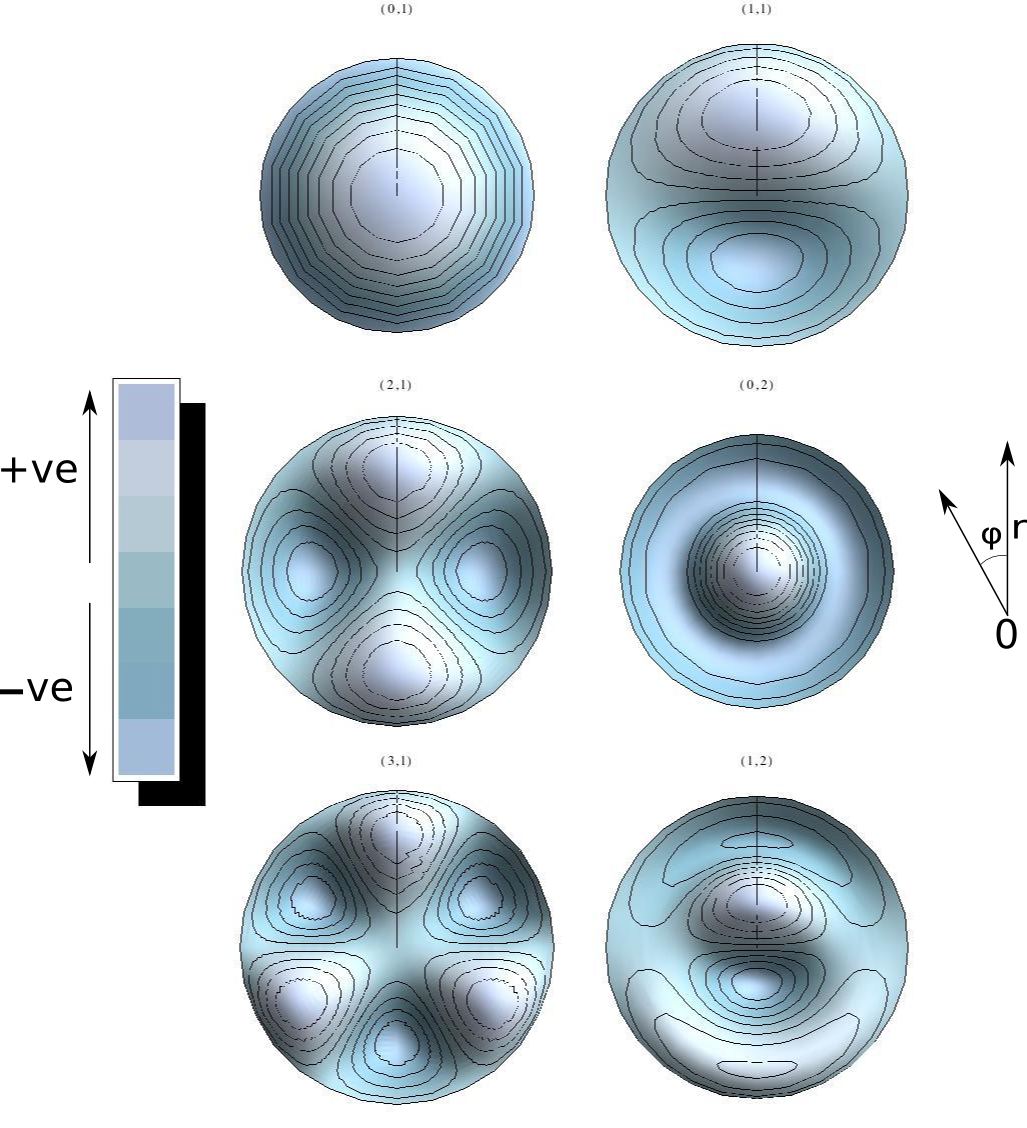
\includegraphics[width=.6\linewidth]{Diagrams/CircularMembraneModes/circular_modes_all.png}
 \caption[Circular membrane eigenmodes]{Eigenmodes of a full circular membrane. The eigenfrequency increases from left to right.}
  \label{circularmembraneeigenmodes}
\end{figure}

We note that unlike in the case of the internal cavity, the free membrane has components
that are both forward- and backward-moving in time. The presence of a driving force, however, will result in simpler expressions. This
will be discussed in more detail in the next chapter where we compare our model with experimental data.

\vspace{\baselineskip}
\noindent\textbf{Damped Membrane}: For a damped membrane, i.e. $\alpha\neq 0$, the spatial part of the above eigenmodes remains the same. The form of the
time-dependent part is given by the solution of the equation,
\begin{equation}\label{dampedtimepart}
 \frac{d^2 h_{mn}(t)}{dt^2}+2\alpha \frac{d h_{mn}(t)}{dt}+\omega_{mn}^2h_{mn}(t)=0.
\end{equation}
Assuming $h_{mn}$ takes the form $e^{j\widetilde{\omega}_{mn}}$ leads to a quadratic equation with solutions,
\begin{align}
 \widetilde{\omega}_{mn}&=j\alpha\pm\omega_{mn}^*\\
 \omega_{mn}^*&=\sqrt{\alpha^2+\omega^2_{mn}}
\end{align}
We require the membrane displacement to remain finite as $t\rightarrow\infty$. We can therefore neglect the $e^{-j\widetilde{\omega}_{mn}}$ terms leading
to,
\begin{equation}\label{circularmembranedampedeigen}
 \widetilde{u}_{mn}(r,\phi;t)=\cos m\phi J_m(\mu_{mn} r)\left[M_{mn}e^{j\omega_{mn}^* t}+N_{mn}e^{-j\omega_{mn}^* t}\right]e^{-\alpha t}
\end{equation}
The general solution is given by a linear combination of the above and the coefficients are determined by initial conditions -- for example,
membrane displacement and velocity at $t=0$.
\subsubsection*{Forced Vibrations}
For a periodically driven membrane, there are two components of the full solution for forced vibrations. The first of these is the steady state solution which
oscillates with the same frequency as the input and does not depend on the initial conditions - $u_{ss}$. The second of these is the transient solution that depends
on the initial conditions but not on the driving pressure - $u_t$. 

\noindent\textbf{Steady State Solution}: The steady state solution is expressed as a linear combination of the spatial part
of the above eigenmodes and is given by,
\begin{equation}\label{membraness1}
 u_{ss}(r,\phi ;t)=\displaystyle\sum^\infty_{m=0}\sum^\infty_{n=1} C_{mn}\cos m\phi J_m(\mu_{mn} r)e^{j\omega t}.
\end{equation}
Substituting this expression in \eqref{membraneequation1} with $\Psi=pe^{j\omega t}$ gives,
\begin{align}
 &\displaystyle\sum^\infty_{m=0}\sum^\infty_{n=1} \Omega_{mn}C_{mn}\cos m\phi J_m(\mu_{mn} r)e^{j\omega t}=pe^{j\omega t}\label{membraness2}\\
 &\text{where,  }\Omega_{mn}=\rho_M d \left[(\omega^2-\omega^2_mn)-2j\alpha\omega\right]\label{omegafirstdef}.
\end{align}
Using the orthogonality of the eigenmodes, the coefficients $C_{mn}$ can be calculated,
\begin{equation}\label{sscoeffs}
 C_{mn}=\frac{p\int dS u_{mn}}{\Omega_{mn}\int dS u^2_{mn}}
\end{equation}
with the integral this time being taken over the circular disk of radius $a_M$.

\vspace{\baselineskip}
\noindent\textbf{Transient Solution}: The transient solution is effectively a solution of the free damped membrane, i.e. a linear 
combination of the eigenmodes given in \eqref{circularmembranedampedeigen}. Therefore,
\begin{equation}\label{membranet1}
 u_t(r,\phi;t)=\displaystyle\sum^\infty_{m=0}\sum^\infty_{n=1}\cos m\phi J_m(\mu_{mn} r)\left[M_{mn}e^{j\omega_{mn}^* t}+N_{mn}e^{-j\omega_{mn}^* t}\right]e^{-\alpha t}.
\end{equation}
The complete solution is given by $u=u_t+u_{ss}$ and the coefficients $M_{mn}$ and $N_{mn}$ are determined by the initial conditions (at $t=0$).

\vspace{\baselineskip}
\textbf{Steady State Approximation}: The damping coefficient $\alpha$ is usually given in terms of the membrane fundamental frequency and a quality factor $Q$ as $\alpha=\omega_{01}/2Q$. For the tympani
we will be concerned with we have $Q\sim 1.2$ which results in damping coefficients that are around $4000s^{-1} $ for the larger lizards and around $8000s^{-1}$ for the smaller ones. 
Due to this and the exponential decay of the transient vibration amplitude, we can safely assume that within a few time-periods the steady-state vibrations dominate the solution of the
forced membrane. For this reason, we will subsequently confine our discussion to only the steady state vibrations of the membrane.
\subsubsection{Sectoral Membrane}
The eigenmodes of the sectoral membrane proceeds from \eqref{membraneeigen} onwards. We now have a new set of boundary conditions in $\phi$.
The extracolumella is modelled as a triangular plate of infinite mass which constrains the membrane displacement to go to zero at $phi=\beta$
and $\phi=2\pi-\beta$. This results in the following set of eigenmodes,
\begin{equation}\label{sectoraleigenmode}
 u_{mn}(r,\phi;t)=\sin \kappa(\phi-\beta) J_\kappa(\mu_{mn} r)\left[M_{mn}e^{j\omega_{mn} t}+N_{mn}e^{-j\omega_{mn} t}\right]
\end{equation}
where $\kappa[m]=\frac{m\pi}{2(\pi-\beta)}$, $m=1,2,3,\ldots$. We see that the $r$ part of the above mode is given by the
order-$\kappa$ Bessel function of the first kind; $\mu_{mn}$ being its $n^{th}$ zero, as before. The solution for the damped
membrane follows in an identical way.
It is apparent from the form of the above modes that, unlike in the case of the circular membrane eigenmodes, these modes
are no longer circularly symmetric. We plot the first few of these modes in \ref{sectoralmembraneeigenmodes}. 
\begin{figure}[ht!]
 \centering
 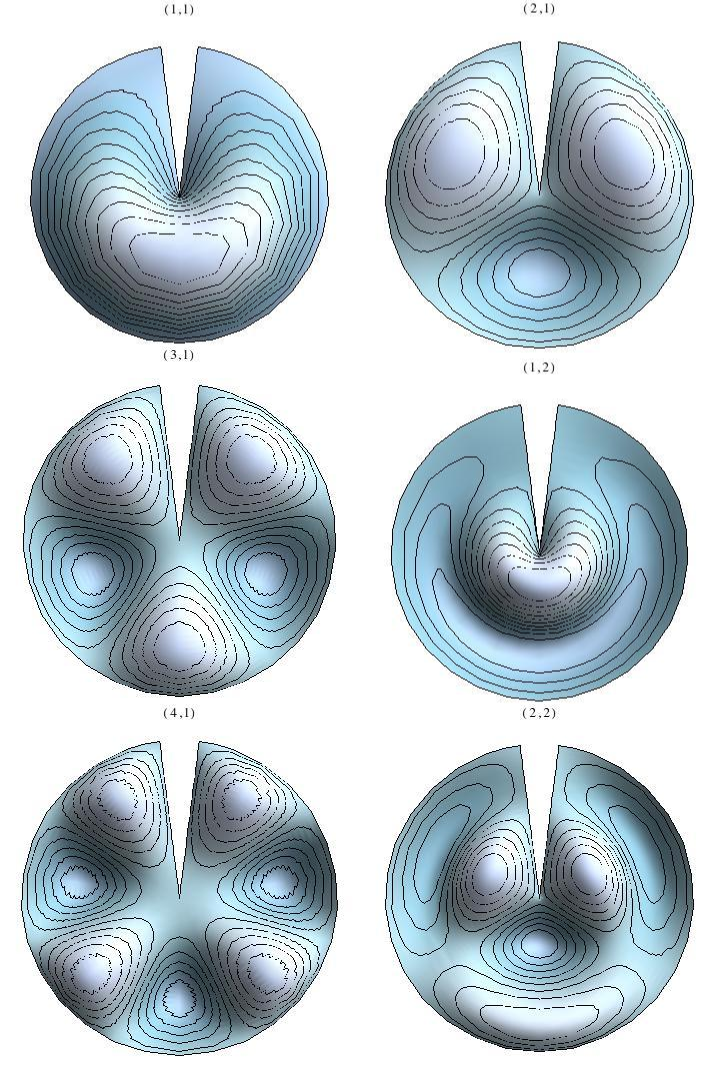
\includegraphics[width=.6\linewidth]{Diagrams/SectorMembraneModes/membrane_modes_all.png}
 \caption[Sectoral membrane eigenmodes]{Eigenmodes of a sectoral membrane where the omitted region corresponds to the extracolumella with $\beta=\pi/25$. As in Fig. \ref{circularmembraneeigenmodes}, the eigenfrequency increases from left to right.}
  \label{sectoralmembraneeigenmodes}
\end{figure}
The solution for forced membrane vibrations follows in the same way as in the circular membrane case. The vibrations of a sectoral membrane
are discussed in more detail in \cite[p.~87]{fletcheracoustic}. As discussed earlier, the sectoral shape of the membrane has important
physical consequences and captures the complex vibration patterns of a realistic membrane. This will be discussed in the next chapter.
\subsection{Vibration of Coupled Membranes}\label{coupledmembranes}
With our current knowledge, we can move on to the main part of the chapter - the vibration of coupled membranes.
It is convenient to first write down the main equations of the system based on our previously derived expressions.
The vibrations of the membranes is given by,
\begin{equation}\label{coupledmembraneseries}
 u_{0/L}(r,\phi;t)=\displaystyle\sum^{\infty}_{m=0}\sum^{\infty}_{n=1}\Omega_{mn}C^{0/L}_{mn}u_{mn}(r,\phi)e^{j\omega t}=p_{0/L}e^{j\omega t}-p(0/L,r,\phi;t)
\end{equation}
where $0$ and $L$ denote the ipsi- and contra-lateral membranes respectively and the cavity pressure distribution, $p(x,r,\phi;t)$,  is given by \eqref{pressuregeneral1}.
The above equation is only valid on the membrane surface i.e., for $r<a_{tymp}$ and $\beta<\phi<2\pi-\beta$.

As discussed in \ref{pressureboundaryconditions}, the internal cavity pressure satisfies the no-penetration condition at solid boundaries.
This means that at both ends of the cylinder, we equate the velocity profile of air to the velocity profile of the circular surface including
the membrane. This is because the membrane diameter is smaller than the cylinder diameter. As a result, we will have to set the air-particle velocity to zero for $r>a_{tymp}$. 
Since the membrane displacement is
only in the $x$-direction, we only need to calculate the same component of the velocity. Using the relation \eqref{pressurevelocityrelation} we get,
\begin{equation}\label{airvelocity}
v_x(x,r,\phi;t)=-\frac{1}{\rho\omega}\displaystyle\sum^\infty_{q=0}\displaystyle\sum^\infty_{s=0}\zeta_{qs}\left(A_{qs}e^{j\zeta_{qs}x}-B_{qs}e^{-j\zeta_{qs}x}\right)f_{qs}(r,\phi)e^{j\omega t}
\end{equation}
and the exact boundary conditions are given by,
\begin{align}
 j\omega U_{0}&=-v_x(0,r,\phi;t)\label{bc1}\\
 j\omega U_{L}&=v_x(L,r,\phi;t)\label{bc2}
 \end{align}
where we've used the direction conventions described in \ref{description} and made the following definition,
\begin{equation}
 U_{0/L}=\begin{cases}
          u_{0/L}\mbox{, } 0<r<a_{tymp}\mbox{ and } \beta<\phi<2\pi-\beta\\
          0\mbox{, otherwise}
         \end{cases}.
\end{equation}
This in order to ensure that the boundary condition is satisfied over either end of the cylinder and not just over the membrane surface.
\subsubsection{Approximate Boundary Condition}
As previously stated, the exact boundary condition would entail setting the velocity function to be exactly equal to the membrane displacement velocity. At this point, it is important to
note that the internal cavity eigenmodes are \textbf{not} orthogonal to the membrane eigenmodes in general\footnote{This would also be true if we had full circular membranes on either end of the
cylinder. In this case we would have the added simplification that only the circularly symmetric cavity eigenmodes will be activated.}. This means that every membrane eigenmode
couples with every cavity eigenmode and that each of the coefficients $A_{qs}$ and $B_{qs}$ will be given by an infinite linear combination of the coefficients $C^{0/L}_{mn}$. 

The first step in overcoming this problem is to rewrite the left-hand sides of the boundary conditions given in \eqref{bc1} and \eqref{bc2}.
We first expand $U_{0}$ and $U_{L}$ in the orthogonal basis of the functions $f_{qs}$,
\begin{align}
 U_{0/L}(r,\phi;t)&=\displaystyle\sum^\infty_{q=0}\displaystyle\sum^\infty_{s=0} S^{0/L}_{qs}f_{qs}(r,\phi)e^{j\omega t}\\
 \mbox{where, }S^{0/L}_{qs}&=\frac{\int dS U^{0/L}f_{qs}(r,\phi)}{\int dS f^2_{qs}(r,\phi)}\label{approxboundarydef2}
\end{align}
We now have an expansion that approximates the boundary condition with increasing accuracy. After choosing an appropriate cutoff
for the expansion we can substitute this expression in place of $U_{0/L}$ in \eqref{bc1} and \eqref{bc2}. In fact, this cutoff in
the boundary condition expansion results in an identical cutoff in the pressure expansion - a direct result of the orthogonality
of the pressure modes. 

We will now illustrate a solution to the problem by solving the problem with the zeroeth order boundary conditions. 
In the end, it will turn out that for our purposes the zeroeth order, i.e. the $(0,0)$ mode is sufficient as higher modes only have a significant contribution at frequencies
well above the hearing range of geckos. For example, the wavenumber of the $(1,1)$ mode is above $33$kHz for the cylindrical cavity corresponding to the house gecko and 
above $15$kHz for the one corresponding to the Tokay gecko. The parameters used to derive these quantities will be discussed in the next chapter.
We can therefore write the approximate boundary conditions to zeroeth order as,
\begin{align}
   \rho\omega^2S^{0}&=-\displaystyle\sum^\infty_{q=0}\displaystyle\sum^\infty_{s=0}j\zeta_{qs}\left(A_{qs}-B_{qs}\right)f_{qs}(r,\phi) \label{bcfinal1}\\
   \rho\omega^2S^{L}&=\displaystyle\sum^\infty_{q=0}\displaystyle\sum^\infty_{s=0}j\zeta_{qs}\left(A_{qs}e^{j\zeta_{qs}L}-B_{qs}e^{-j\zeta_{qs}L}\right)f_{qs}(r,\phi) \label{bcfinal2}
\end{align}
As shown in Sec. \ref{internalcavity}, the $(0,0)$ mode only varies in the $x$-direciton.
As a result, the left-hand sides of
the above equation are nothing but the average displacement of the membrane surface given by,
\begin{equation}\label{averagemembranedisp}
 S^{0/L}=\frac{\int dS U^{0/L}(r,\phi)}{\pi a^2_{cyl}}.
\end{equation}
We have also omitted the ``$qs$'' subscript from $S^{0/L}$. 
Given the external parameters and boundary conditions, it only depends on time.
We have effectively approximated the surfaces at $0$ and $L$ (including the membranes) by pistons moving with the average velocity of the total surface.

Given these boundary conditions, it is straightforward to calculate the coefficients $A_{qs}$ and $B_{qs}$ in terms of $S_{0/L}$. To do this
we need to make use of the orthogonality relation given in \eqref{besselorthogonality}. We do this by multiplying both sides of \eqref{bcfinal1} and \eqref{bcfinal2}
by $f_{qs}(r,\phi)$ and integrate over the circular surfaces at either end of the cylinder. This results in a system of two linear equations for each pair of $A_{qs}$ 
and $B_{qs}$,
\begin{align}
 &A_{qs}-B_{qs} = -L_{qs}\rho\omega^2S^{0}\\
 &A_{qs}e^{j\zeta_{qs}L}-B_{qs}e^{-j\zeta_{qs}L} =  L_{qs}\rho\omega^2S^{L}\\
 \mbox{where,}\ &L_{qs} = \frac{\int dS f_{qs}(r,\phi)}{j\zeta_{qs}\int dS f^2_{qs}(r,\phi)}\nonumber
\end{align}
We now make use of the property of the pressure modes that $f_{qs}(r,\phi)$ integrates to $0$ unless $q=0$ and $s=0$. 
For $q=0$ this is a consequence of the Bessel functions integrating to zero while for $q\geq 1$ this is due to 
the more obvious fact that the integral of the cosine function from $0\mbox{ to }2\pi$ is zero. As a result we have $A_{qs}=B_{qs}=0$ for all
modes except the $(0,0)$ mode. In other words, the zeroeth-order boundary condition only supports plane wave
modes inside the cavity. We will subsequently omit the subscripts ``$00$'' for these coefficients.
From the above linear equations, they are given in terms of the total membrane displacement as,
\begin{equation}\label{finalpressurecoefficients}
 A=-\frac{\rho\omega^2}{2 k\sin kL}\left(S^0e^{-jkL}+S^L\right),\qquad  B=-\frac{\rho\omega^2}{2 k\sin kL}\left(S^0e^{jkL}+S^L\right)
\end{equation}
we have also directly substituted $\zeta_{00}=k$ and simplified the expression for $K_{00}$ in the above expressions. These
coefficients can now be substituted in place of the pressure in the right-hand side of the equation \eqref{coupledmembraneseries}
giving us,
\begin{align}
 &\displaystyle\sum^\infty_{m=0}\displaystyle\sum^\infty_{n=1}\Omega_{mn}C^{0}_{mn}u_{mn}(r,\phi)=p_{0}+\frac{\rho\omega^2}{k}\left(S^0\cot kL+S^L\csc kL\right)\\
 &\displaystyle\sum^\infty_{m=0}\displaystyle\sum^\infty_{n=1}\Omega_{mn}C^{L}_{mn}u_{mn}(r,\phi)=p_{L}+\frac{\rho\omega^2}{k}\left(S^0\csc kL+S^L\cot kL\right)
\end{align}
where we have cancelled out the time component on both sides of the equations. Note that the right-hand sides of the above two equations
are independent of the spatial $(r,\phi)$ coordinates.

In order to simplify the above coupled system of equations, the next step will be to take their sum and difference to obtain a new set of 
variables that are solutions of a pair of decoupled equations. After some algebraic manipulation, we therefore have
\begin{align}
 &\displaystyle\sum^\infty_{m=0}\displaystyle\sum^\infty_{n=1}\Omega_{mn}C^{+}_{mn}u_{mn}(r,\phi)=p_{+}+\frac{\rho\omega^2}{k}S^+\cot \frac{kL}{2}\\
 &\displaystyle\sum^\infty_{m=0}\displaystyle\sum^\infty_{n=1}\Omega_{mn}C^{-}_{mn}u_{mn}(r,\phi)=p_{-}-\frac{\rho\omega^2}{k}S^-\tan \frac{kL}{2}
\end{align}
where, $C_{mn}^+=C_{mn}^L+C_{mn}^0$ and $C_{mn}^-=C_{mn}^L-C_{mn}^0$. The $S^{+/-}$ and $p_{+/-}$ terms are defined similarly.
Now, analogous to the calculation of the coefficients for the steady state vibration in \eqref{membraness2} and \eqref{sscoeffs}, we can determine
the coefficients of the sum and difference vibrations in terms of the pressure and total membrane displacements. This gives us,
\begin{align}
 C^{+}_{mn}&=\left[p_{+}+\frac{\rho\omega^2}{k}S^+\cot \frac{kL}{2}\right]K_{mn}\label{pluscoeffdef}\\
 C^{-}_{mn}&=\left[p_{-}-\frac{\rho\omega^2}{k}S^-\tan \frac{kL}{2}\right]K_{mn}\label{minuscoeffdef}\\
 \mbox{where, }K_{mn}&=\frac{\int dS u_{mn}}{\Omega_{mn}\int dS u^2_{mn}}\nonumber
\end{align}
The next step will be to multiply both sides of \eqref{pluscoeffdef} and \eqref{minuscoeffdef} with the integral $\int dS u_{mn}$, 
divide by $\pi a^2_{cyl}$ (the integral of $f^2_{00}$ as it appears in the denominator in \eqref{approxboundarydef2}) and
sum over $m\mbox{ and }n$ . It is clear that the left hand sides become equal to $S^{+/-}$; this allows us to give exact expressions
for the total membrane displacements.
\begin{equation}
 S^{+}=\frac{p_L+p_0}{\Lambda+\Gamma_+}\qquad S^{-}=\frac{p_L-p_0}{\Lambda+\Gamma_-}
\end{equation}
where we've defined the following quantities,
\begin{align}
 \Gamma_+ = -\frac{\rho\omega^2}{k}\cot \frac{kL}{2},\qquad \Gamma_-= \frac{\rho\omega^2}{k}\tan \frac{kL}{2}\nonumber
,\qquad\frac{1}{\Lambda}=\frac{1}{\pi a^2_{cyl}}\displaystyle\sum^\infty_{m=0}\displaystyle\sum^\infty_{n=1}\frac{\left(\int dS u_{mn}\right)^2}{\Omega_{mn}\int dS u^2_{mn}}\nonumber
\end{align}
We can finally write the membrane displacement as a function of the pressure inputs in the form
\begin{align}
 u_0(r,\phi;t)&=G_{ipsi}(r,\phi)p_0+G_{contra}(r,\phi)p_L\label{ipsimembranefull}\\
 u_L(r,\phi;t)&=G_{contra}(r,\phi)p_0+G_{ipsi}(r,\phi)p_L\label{contramembranefull}
\end{align}
with the ipsilateral filter,
\begin{equation}
 G_{ipsi}=\left(\frac{1}{\Lambda+\Gamma_+}+\frac{1}{\Lambda+\Gamma_-}\right)\displaystyle\sum^\infty_{n=1}\frac{\Lambda K_{mn}}{2}u_{mn}(r,\phi;t)
\end{equation}
and the contralateral filter,
\begin{equation}
 G_{contra}=\left(\frac{1}{\Lambda+\Gamma_+}-\frac{1}{\Lambda+\Gamma_-}\right)\displaystyle\sum^\infty_{n=1}\frac{\Lambda K_{mn}}{2}u_{mn}(r,\phi;t)
\end{equation}
The total membrane displacement can also be expressed as a function of $p_0$ and $p_L$ simply by integrating both sides of \eqref{ipsimembranefull}
and \eqref{contramembranefull} giving us a new set of ipsi- and contralateral filters
\begin{align}
 G^s_{ipsi}&=\left(\frac{1}{\Lambda+\Gamma_+}+\frac{1}{\Lambda+\Gamma_-}\right)/2 \label{ipsimembranetotal}\\
 G^s_{contra}&=\left(\frac{1}{\Lambda+\Gamma_+}-\frac{1}{\Lambda+\Gamma_-}\right)/2 \label{contramembranetotal}
\end{align}
The ipsilateral filter effectively gives us the response of the ipsilateral membrane when the contralateral membrane
is blocked. Similarly, the contralateral filter gives us its response when there is no ipsilateral stimulus. These filters
will play an important role in the evaluation of the model in the next chapter.

\subsection{Circuit Model}
Before we conclude this chapter, we will discuss the previous methods used to model ears coupled through
an air cavity. This method was used by Christensen-Dalsgaard and Manley in \cite{dalsgaardmanley1} and \cite{dalsgaardmanley2}
and was based on methods presented in \cite{fletcheracoustic}. The method treats the problem through the analogy of electrical circuits
and deals with low-frequency and high-frequency regimes separately.

In these models, the sound inputs are treated as voltage sources and the system is broken down into components, e.g.	 membranes,
cavities, apertures which are modelled as lumped elements. Their impedance values depend on the geometry and material properties and in general
 can be resistive and reactive. The ``current'' is given by something called the ``acoustic flow'' which has the dimensions of
volume per unit time. In the previous analysis, this is given by $j\omega\pi a^2_{cyl}S^{0/L}$. 

The low frequency circuit analog for the ICE model is illustrated in Fig. \ref{lowfreqcircuit}. The impedances are calculated
using the following formulae,
\begin{align}
 &R_T=\frac{\omega_TL_T}{Q},\qquad L_T=\frac{\rho_Md}{\pi a_{tymp}^2},\qquad C_T=\frac{1}{\omega^2_TL_T}\\
 &R_V=0,\qquad L_V=0,\qquad C_V=\frac{V_0}{\rho c^2}
\end{align}
where $R,\ L\mbox{ and }C$ are the resistance, impedance and capacitance of the quantities respectively with the total impedance
given by $Z=R+j\omega L+1/j\omega C$. $\omega_T$ is the first eigenfrequency of the membrane.
\begin{figure}[ht!]
 \centering
 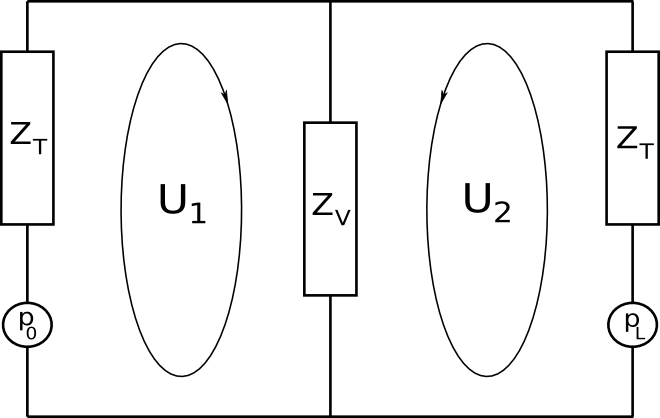
\includegraphics[width=.5\linewidth]{Diagrams/lowfreqcircuit.png}
 \caption[Low frequency circuit analog]{Low frequency circuit analog for the ICE-Model. The membrane impedences are denoted by $Z_T$ and the impedance of 
 the internal cavity is denoted by $Z_V$. The acoustic flows are given by $U_1\mbox{ and }U_2$.}
  \label{lowfreqcircuit}
\end{figure}
It should immediately be apparent that the cavity impedance only depends on its volume. This is a result of the assumption 
that the air inside the cavity behaves like an adiabatic gas. The adiabatic equation of state can then be used
to determine the instantaneous pressure from the instantaneous volume change due to the membrane
motion which, after linearization, results in a uniform pressure inside the cavity. In addition, the membrane impedance $Z_T$ only includes the
effect of the first eigenmode. Also, $Z_T$ includes the effect of the transducer which, in our case, is the extracolumella. Upon solving the circuit equations, the acoustic flows are calculated to be,
\begin{equation}
 U_1=\frac{p_0(Z_T+Z_V)-p_LZ_V}{Z_T(Z_T+2Z_V)},\qquad U_2=\frac{p_L(Z_T+Z_V)-p_0Z_V}{Z_T(Z_T+2Z_V)}.
\end{equation}
At first glance the above results look very similar to total membrane displacements shown in \eqref{ipsimembranefull} and \eqref{contramembranefull}.
In fact, we can find the equivalent impedances from our analysis by comparing $U_0$ and $U_L$ with the above results,
\begin{equation}
 Z^{eq}_T=\frac{1}{j\omega\pi a^2_{cyl}}(\Lambda+\Gamma_-),\qquad Z^{eq}_V=\frac{1}{2j\omega\pi a^2_{cyl}}(\Gamma_+-\Gamma_-)
\end{equation}
We immediately see that in the equivalent membrane impedance there is a correction term, $\Gamma_-$, which is a result of the contribution of the cavity whereas in 
the circuit model, the membrane impedance is determined independent of the cavity. Moreover, the equivalent standalone membrane impedance, $\Lambda$,
includes the influence of the higher modes. The equivalent cavity impedance becomes equal to $Z_V$ at zero frequency and goes to infinity at the
resonance frequencies of the cylinder, i.e at $\omega=n\pi c/L,\ n=1,2\ldots$.
% At high frequencies, i.e. when the wavelength of the input becomes comparable with the dimensions of the system, the description of the
% membrane does not change but the cavity impedance has a frequency dependent addition instead modelled as a two-port network. 
% 
% \begin{figure}[ht!]
%  \centering
%  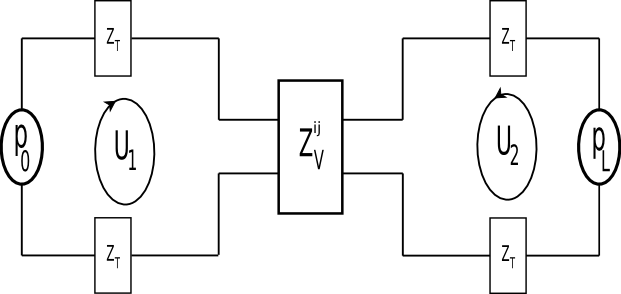
\includegraphics[width=.75\linewidth]{Diagrams/highfreqcircuit.png}
%  \caption[High frequency circuit analog]{High frequency circuit analog for the ICE-Model.}
%   \label{highfreqcircuit}
% \end{figure}
\vspace{\baselineskip}

\noindent We conclude this chapter by briefly stating the advantages of our method in comparison to the lumped element method - 
\begin{itemize}
 \item In terms of the membrane motion - we are able to account for the effect of asymetrically loaded extracolumella and are able to describe the membrane motion is spatial detail.
 \item At low frequencies our model is consistent with the uniform pressure assumption but the nonuniformity steadily increases with frequency.
  We therefore have a single model that can describe both high- and low-frequency behaviour instead of treating the two regimes separately.
\end{itemize}


  \chapter{Evaluation of the Model}\label{modelanalysis}
We now have a complete geometrical representation of the ICE model as well as
 the analytical expressions $u_0$ and $u_L$ that describe the membrane displacements
in spatial detail as a function of direction and frequency. In this chapter we will use these variables
to further study the features and predictions of our model and compare them with experimental results. In
order to completely explain the observations, we will also need to estimate certain physical parameters
like membrane eigenfrequency and quality factor that are important to our analysis but haven't yet been
experimentally measured.

The main body of this chapter proceeds in Sec. \ref{localizationsection} directly from the definitions given in \eqref{ipsimembranefull}
and \eqref{contramembranefull}. We will begin by assigning numerical values to the model parameters that have been defined
in the previous chapter and comparing the membrane velocities of our model with experimentally determined values. 
We will then go on to define define and study the two main quantities that serve as important localization
cues - the Internal Time Differences (iTDs) and the Internal Level Differences (iLDs). 
These values model the 
possible neural subtractions that take place in the animal's brain in order to enhance directional sensitivity. Upon obtaining 
the spectral behaviour of these quantities, we will also be able to make an educated guess about
the respective frequency ranges in which these cues are dominant and the possible range in which they could simultaneously
be used. 
We will end this section
by discussing possible methods to estimate parameter values that are difficult to measure.
% A complete evaluation of our model also requires  a discussion of the 
% pressure distribution profile and eigenfrequencies of the mouth cavity which will be done in Sec. \ref{pressuredistchapter}.
Finally, in Sec \ref{vibrationpatternchapter} we will compare the experimentally determined vibration pattern
of the Tokay gecko's eardrum with that of our model's eardrum - the aim being to justify our choice for the
geometry of the membrane.

In order to underline the fact that our model is universal model for internally coupled ears and not
specialized to single species, we will compare our results for two gecko species - \emph{Hemidactylus frenatus}
or the common house gecko and the Tokay gecko. At the end of the chapter we will have an understanding of the advantages of a coupled system of ears as opposed
to a pair of independent ears. We will also have an idea about the frequency regimes that correspond to the use
of iTDs and iLDs in localization.

\section{Sound Localization Using the ICE -Model}\label{localizationsection}
In our study we are primarily concerned with hearing in geckos. We will be using
parameters (interaural separation, tympanum area etc.) from \emph{Hemidactylus frenatus}, the common house gecko
\cite{dalsgaardmanley2} and the Tokay gecko \cite{dalsgaardmanley1}, \cite{dalsgaardtangcarr}. In order to proceed
with our evaluation of our model, we will need to assign appropriate numerical values to the parameters we have
defined in \ref{parametertable}. For now we will simply list the values and leave the discussion to a later point.

\vspace{\baselineskip}
\noindent
\begin{minipage}{\linewidth}
\renewcommand{\arraystretch}{1.3}
%\caption{Parameters and Functions used in the ICE Model} \label{parametertable} 
\centering
\captionof{table}{ICE Model geometry Parameters for the common house gecko (Hemidactylus frenatus) and the Tokay gecko.}\label{geckogeometricparams}
\begin{tabular}{|p{8.5 cm} | c | c|}
\hline
Parameter name & Hemidactylus & Tokay gecko\\
\hline
Length of the cylinder or interaural distance, L & $10$mm & $22$mm\\
Radius of the tympanic membrane, $a_{\mathrm{tymp}}$& $1.6$mm & $2.6$mm\\
Fundamental frequency (first eigenfrequency) of the tympanic membrane, $f_0=\omega_{01}/2\pi$ & $2.8$kHz & $1.05$kHz\\
Quality factor of the tympanum, $Q$ & $1.54$ &  $1.33$\\
Density of the membrane material, $\rho_m$ & $1$mg/mm$^3$ & $1$mg/mm$^3$\\
Thickness of the membrane, $d$& $8\mu$m & $10\mu$m\\
Volume of the cavity, $V_{\mathrm{\mathrm{cav}}}$ & $.32$ml & $3.5$ml\\ 
Extracolumella angle, $\beta$ & $\pi/25$ & $\pi/25$\\
Cylinder radius calculated from $V_{\mathrm{\mathrm{cav}}}$ and $L$ using the formula given in \eqref{cylinderradiusformula}, $a_{cyl}$ & $\sim 3.2$mm  &$\sim 6.6$mm \\
\hline
\end {tabular}\par
\bigskip
\end{minipage}
From these quantities it should be apparent that the house gecko, with an interaural separation of $10$mm and mouth cavity volume of $.32$ml is a rather
small lizard. The Tokay gecko is the second largest gecko species (interaural separation of $22$mm and mouth cavity volume $3.5$ml, \cite{dalsgaardmanley2}).
Thus we will demonstrate the scalability of our model with regards to hearing in animals with widely varying head widths and mouth cavities. As we will subsequently see, the geometric parameters, especially
the head width and the membrane eigenfrequencies, put important limits on the ``hearing range'' of our model.

Before we begin our comparison of the data, we should first acquaint ourselves with some experimental details. As already mentioned in Sec. \ref{soundinput}, the geckos were placed in
an anechoic room. They were subject to $175$ms frequency sweeps (200-7500 Hz) at levels of 80-90 dB with the speakers placed at
a $1$m distance. The eardrum vibrations were then measured using laser-Doppler vibrometry with the point
of measurement at the tip of the extracolumella. The measured values correspond to the displacement velocity of the membrane at this point.  
In our analysis, the point corresponding to the tip of the extracolumella is stationary and cannot be used to compare the vibrations of the membranes. 
Instead, we use the total membrane displacements defined in the previous chapter which are given by,
\begin{align}
 &S^0=G^s_{ipsi}p_0+G^s_{contra} p_L\\
 &S^L=G^s_{ipsi}p_L+G^s_{contra}p_0\\
 &\dot{S}^{0/L}=j\omega S^{0/L}\label{totalvelocity}
\end{align}
using the ipsi- and contralateral filters for the total displacement defined in \eqref{ipsimembranetotal} and \eqref{contramembranetotal}.
The definition of the total membrane velocity given in the second line follows directly from the definition of the membrane displacements. Following Sec. \ref{soundinput}
and \eqref{oldsoundinput}, the sound pressure inputs have the form
\begin{equation}\label{newsoundinput}
 p_0=pe^{j\omega t} e^{j\Delta_{new}/2},\qquad p_L=pe^{j\omega t} e^{-j\Delta_{new}/2},\qquad \Delta_{new}=1.5kL\sin\theta.
\end{equation}
The rest of this section follows from the above definitions. In Sec. \ref{vibvelocity} we study the dependence of the membrane vibration velocity 
on the frequency and direction of the sound source. Using the membrane vibration velocity we will define the main directional hearing cues
 - the Internal Time and Level Differences - in Sec. \ref{hearingcuessection}. As mentioned earlier, we will conclude by justifying our selection of parameters. In
Sec. \ref{parameterestimation} we will analyze the dependence of the expressions defined in previous sections on the system parameters 
and in this way also provide estimates for realistic material parameters.  The code used for all the subsequent simulations is given in \ref{codeappendix}

\subsection{Membrane Vibration Velocity}\label{vibvelocity}
We will first evaluate the variation of the membrane displacements with respect to external 
sound stimuli. Before we begin, we should note that although the quantities
$\dot{S}^{0/L}$ will not quantitatively reproduce the experimentally measure membrane vibrations, their behaviour with respect to
frequency and direction is consistent. They also have the added advantage that they only depend on direction and frequency. In Fig. \ref{hemidactylusvibampfull},
we compare the normalized velocity of the tympanic membrane ($\dot{S}^{0/L}/(\pi a^2_{cyl})$) with the membrane velocity measured using laser vibrometry
in \cite{dalsgaardmanley1} and \cite{dalsgaardmanley2}. The plot shows the vibration amplitude as a function of frequency ($y$-axis) and direction ($x$-axis). The amplitudes are given
is units of dB re $1$ mm/(s Pa). This means that we have plotted the ratio vibration amplitude with reference to a vibration velocity of $1$ mm/s with an input pressure of $1$ Pa.
In other words we have set $p=1$Pa in \eqref{newsoundinput}.
\begin{figure}[ht!]
 \centering
 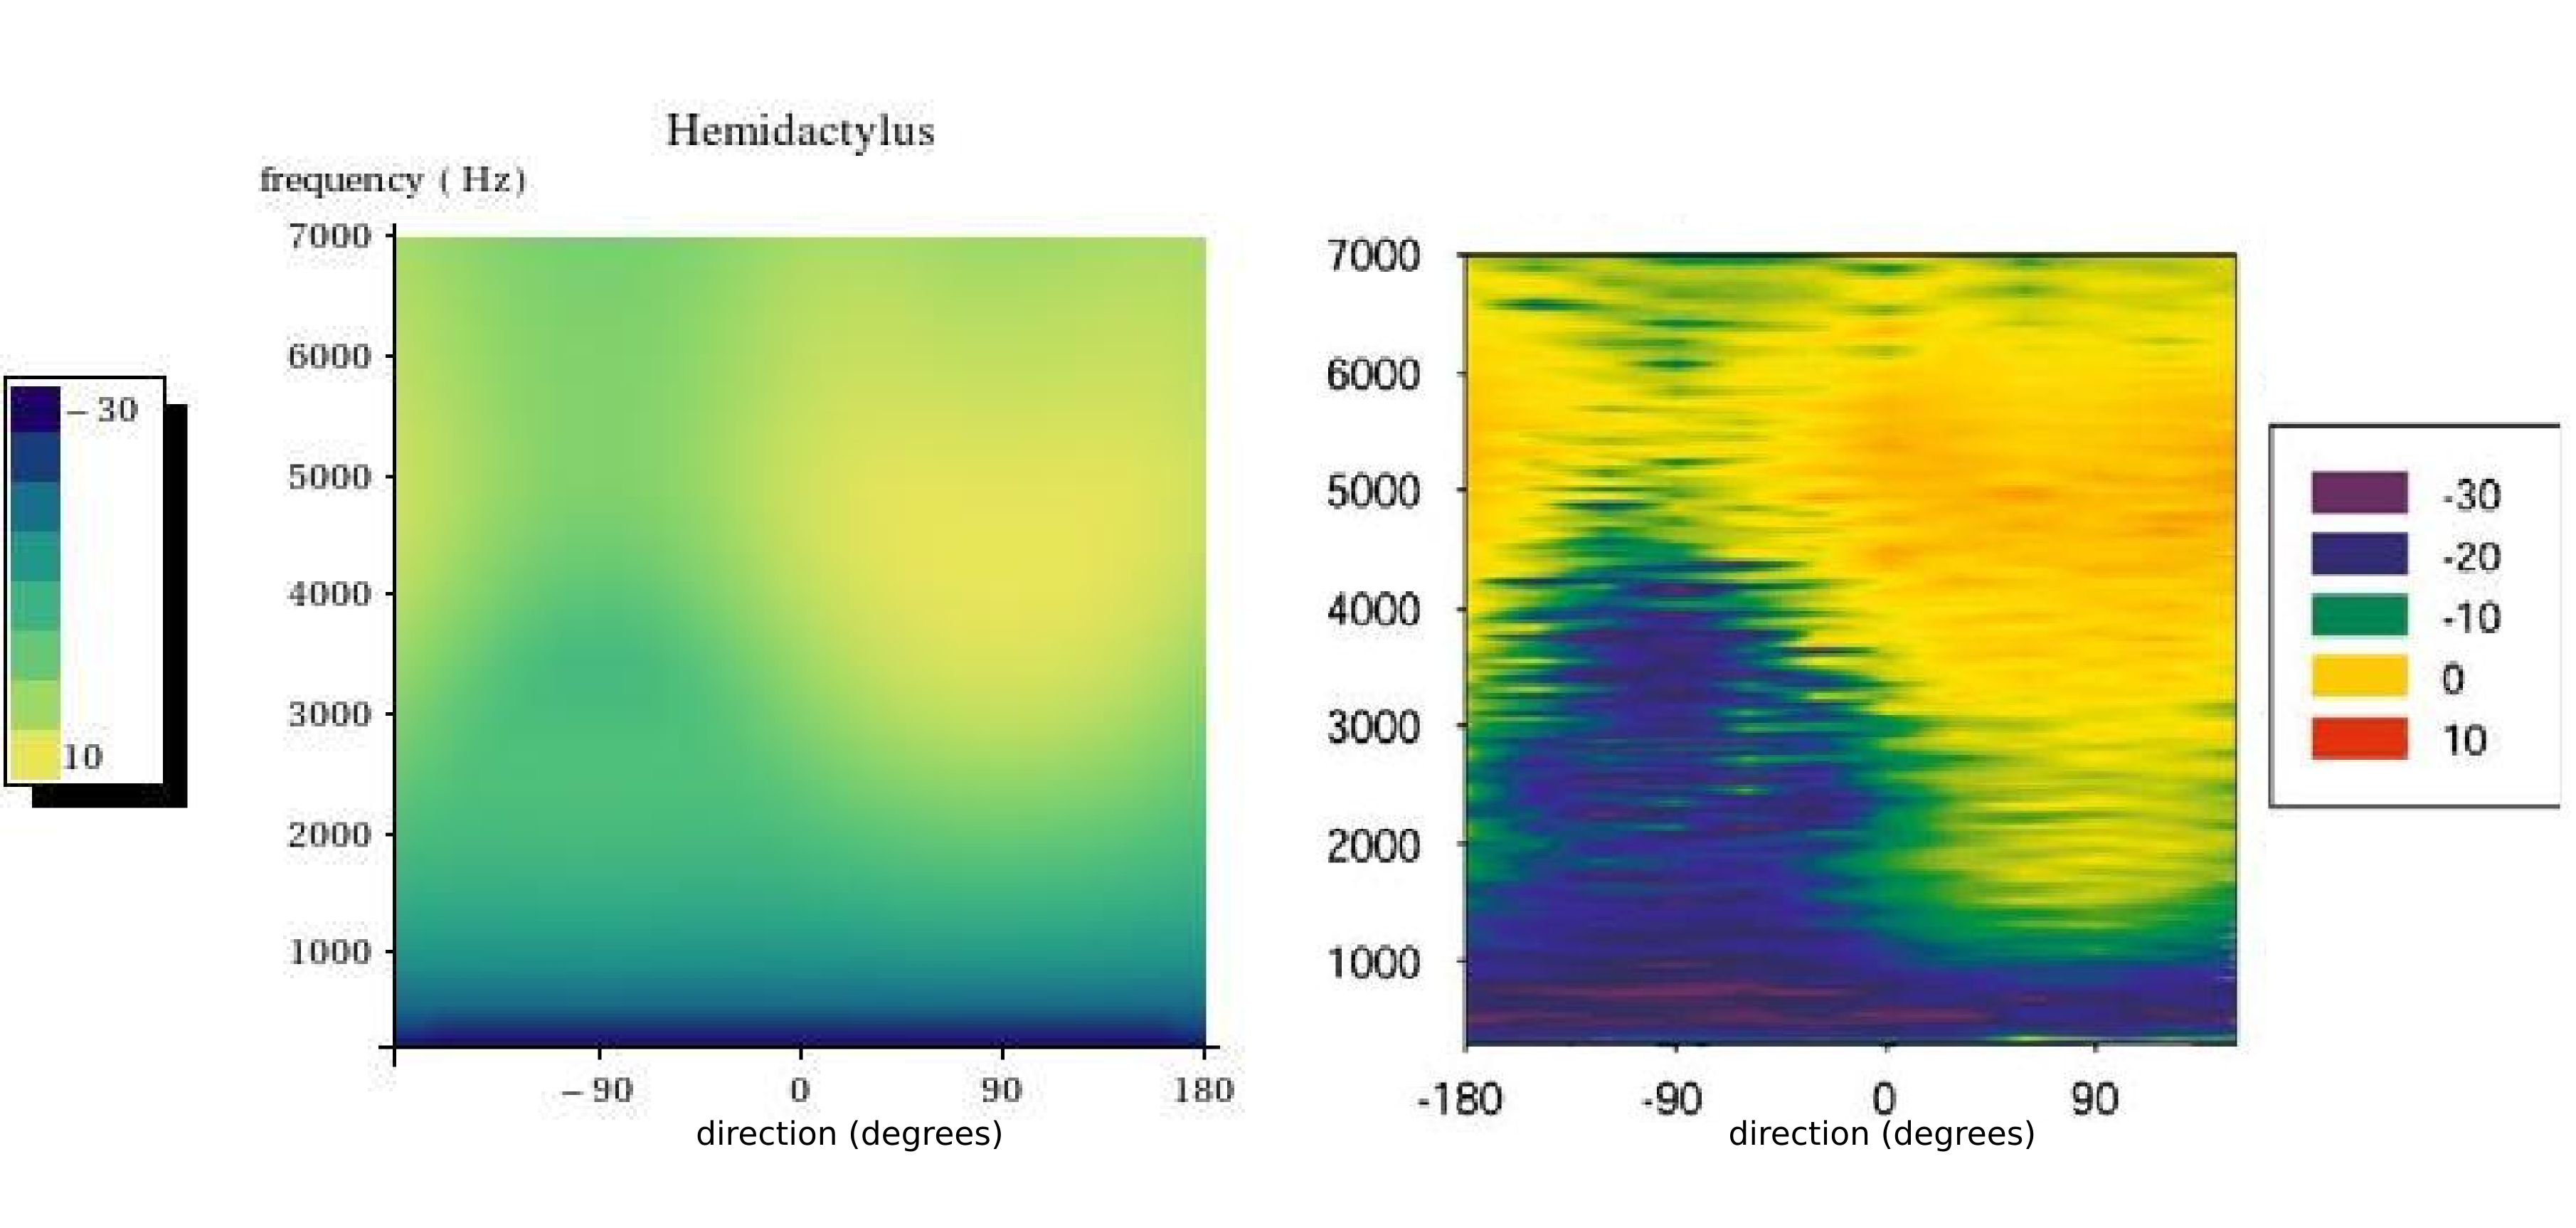
\includegraphics[width=1.0\linewidth]{Diagrams/Plots/hemidactylusvibampfull.png}
 \caption[Vibration amplitude for the common house gecko]{Calculated (left) and experimental (right) amplitude of tympanic membrane vibrations for Hemidactylus frenatus
 in dB re $1$ mm/(s Pa), i.e. the ratio of the vibration amplitude with reference to a vibration velocity of $1$ mm/s with an input pressure of $1$ Pa. On the $x$-axis we have
 the direction of the sound source in degrees varying from $-180^\circ\mbox{ to }180^\circ$ with positive angles corresponding to ipsilateral stimuli. The legends on the left and
 right denote the amplitude in decibels. The calculated values are from the ICE model and the experimental values are taken from Christensen-Dalsgaard \cite{dalsgaardmanley2}.}
  \label{hemidactylusvibampfull}
\end{figure}

As we can see, the total membrane velocities reproduce the frequency and direction dependence of the system fairly well. The directional behaviour is consistent with regard
to the requirement that the membrane have a higher vibration amplitude when it is on the same side as the object. The reason for the deviation from experimental behaviour at 
higher frequencies isn't currently known. The mechanics of the extracolumella including its flection and the influence of the realistic shape of the mouth cavity could offer possible explanations.
Although the room was tested to be anechoic to below $200$Hz some reflections, especially from
the laser setup are unavoidable. This is the cause of the spectral ripple in the experimental measurements. The same comparison is illustrated for the Tokay gecko in Fig. \ref{tokayvibampfull} (data from \cite{dalsgaardmanley1}).
\begin{figure}[ht!]
 \centering
 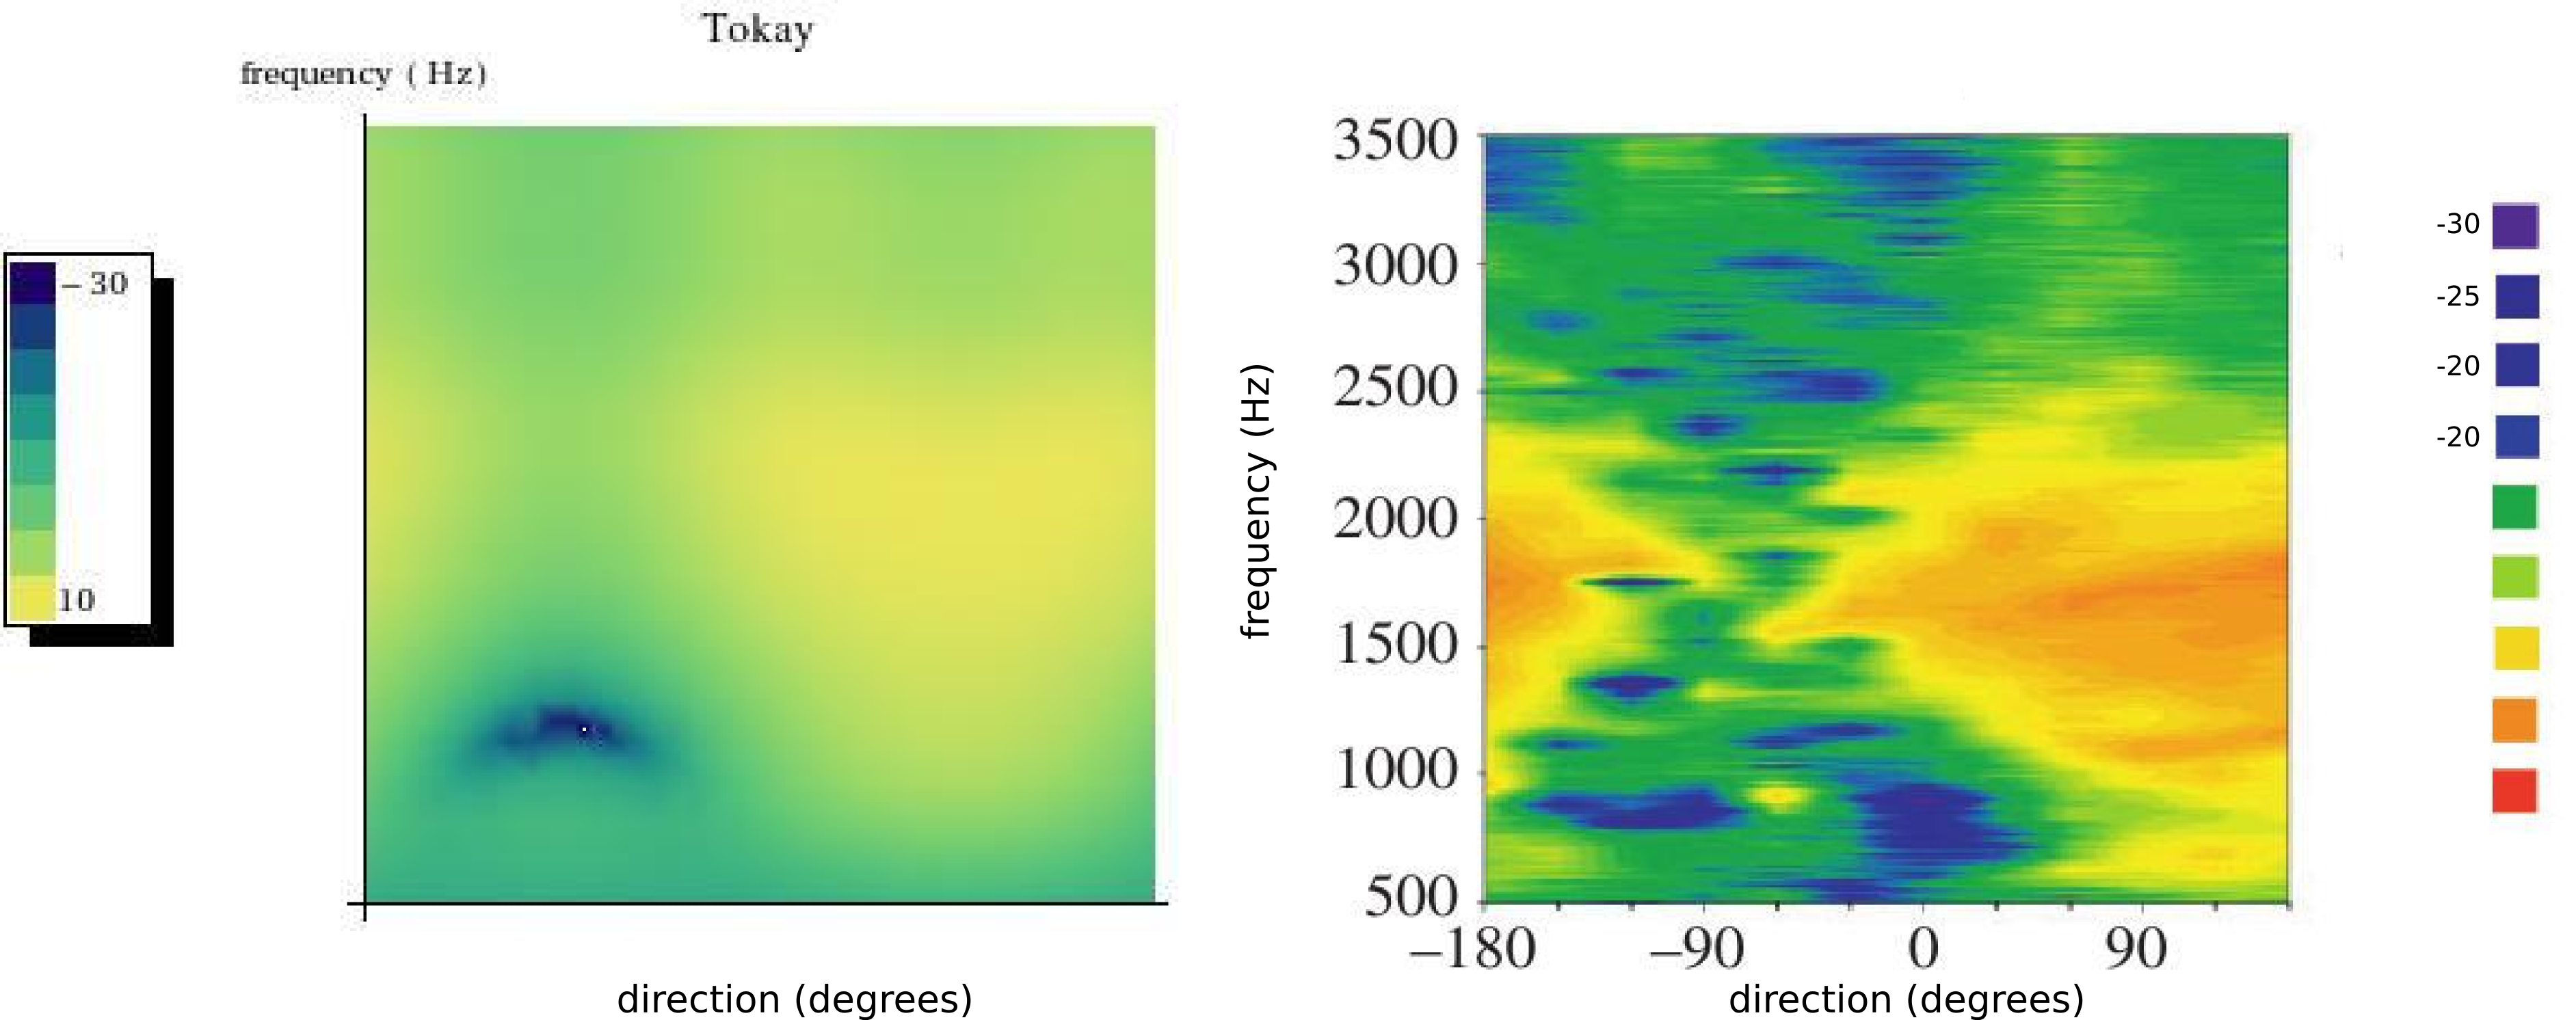
\includegraphics[width=1.0\linewidth]{Diagrams/Plots/tokayvibampfull.png}
 \caption[Vibration amplitude for the Tokay gecko]{Calculated (left) and experimental (right) amplitude of tympanic membrane vibrations for the Tokay gecko
 in dB re $1$ mm/(s Pa). The axis and legend values are the same as the ones in Fig. \ref{hemidactylusvibampfull}. The experimental values are taken from Christensen-Dalsgaard \cite{dalsgaardmanley1}.}
  \label{tokayvibampfull}
\end{figure}

% \begin{figure}[ht]
% \begin{minipage}[b]{0.45\linewidth}
% \centering
% 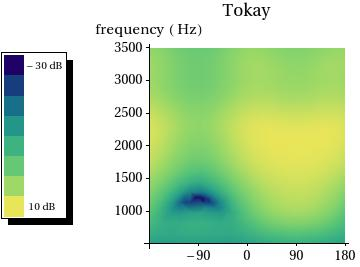
\includegraphics[width=\textwidth]{Diagrams/Plots/tokayvibamp.jpeg}
% \caption{default}
% \label{fig:figure1}
% \end{minipage}
% \hspace{0.5cm}
% \begin{minipage}[b]{0.4\linewidth}
% \centering
% 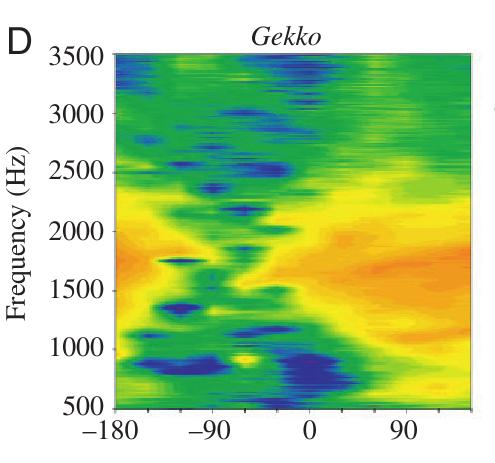
\includegraphics[width=\textwidth]{Diagrams/Plots/tokayvibamp_exp.jpeg}
% \caption{default}
% \label{fig:figure2}
% \end{minipage}
% \end{figure}

In order to get a better understanding of the directionality of the model, it is also important to look at the dependence of the vibration amplitudes on direction and frequency independently. 
In Fig. \ref{hemidactylusipsivscontrafull} (house gecko)
and Fig. \ref{tokayipsivscontrafull} (Tokay gecko) we have plotted the membrane vibration velocity for a pure ipsilateral stimulus (90$^\circ$) and pure contralateral stimulus (-90$^\circ$)
as a function of frequency.
\begin{figure}[ht!]
 \centering
 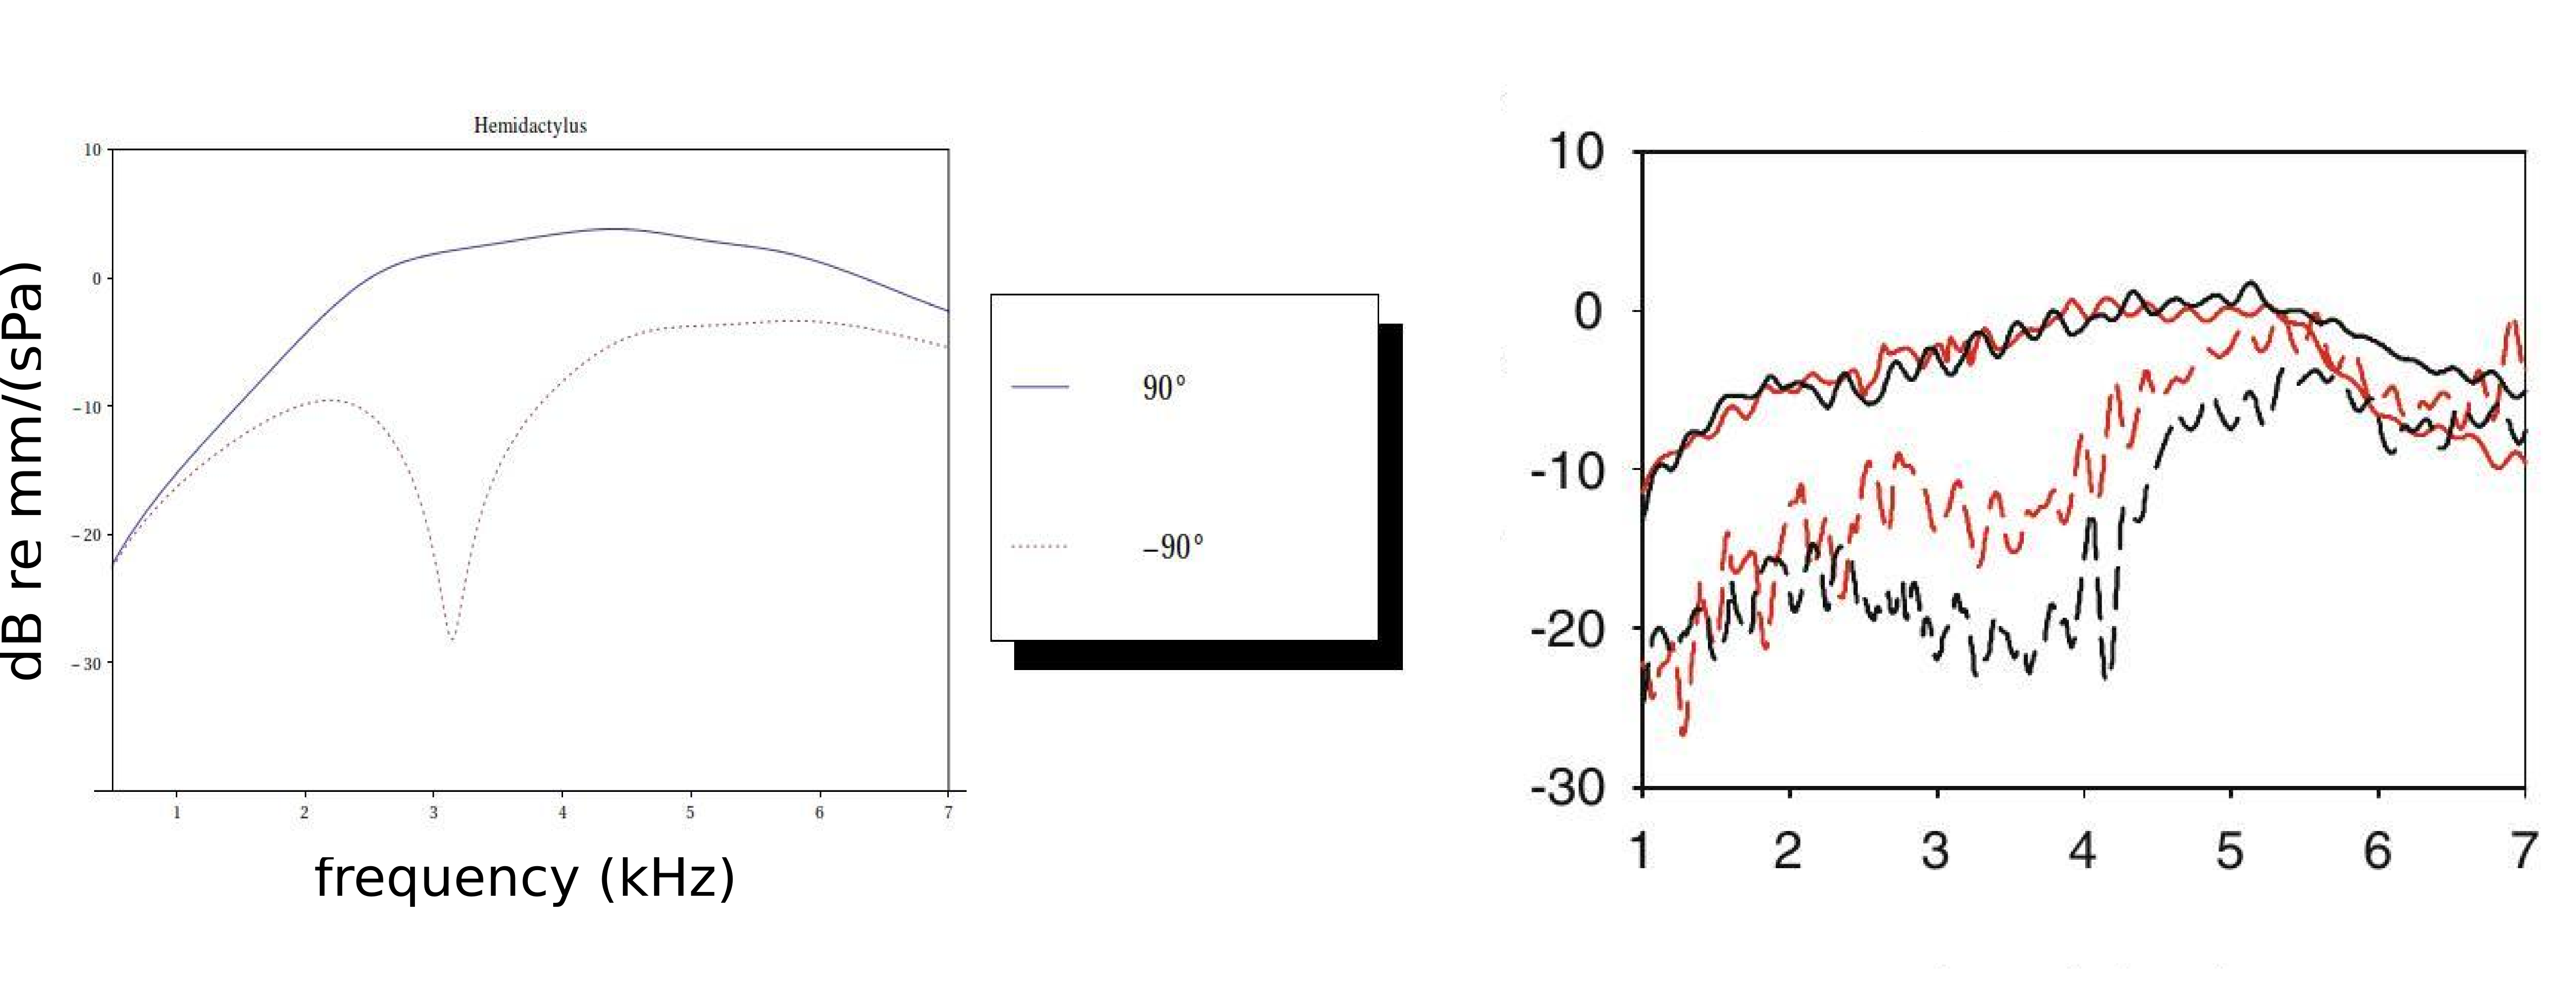
\includegraphics[width=1.0\linewidth]{Diagrams/Plots/hemidactylusipsivscontrafull.png}
 \caption[Frequency dependence of ipsi- and contralateral membrane vibration amplitudes - common house gecko]{Calculated (left) and experimental (right) vibration velocity spectra for the common house gecko. The two plots
 on the left correspond to the response of the tympanic membrane to a purely ipsilateral (90$^\circ$) and purely contralateral (-90$^\circ$) stimulus.  The two colours on the right correspond to
 different individuals of the house gecko species. Experimental values taken from Christensen-Dalsgaard \cite{dalsgaardmanley2}.}
  \label{hemidactylusipsivscontrafull}
\end{figure}
As we can see the ipsilateral response is generally higher than the contralateral response and the difference peaks at a certain frequency i.e., it
has a bandpass characteristic which is consistent with observations.
These amplitude differences can be used to localize the sound source; see Sec. \ref{hearingcuessection}. At very low and very high frequencies the both the vibration amplitudes
converge.  In Fig. \ref{freqdepboth} we  have also plotted the response of the ear to ipsi- and contralateral stimuli with varying directions. (90$^\circ$,60$^\circ$,0$^\circ$,-60$^\circ$,-90$^\circ$)
and thereby shown that the vibration amplitude is higher when the sound source is nearer to the ear (i.e. $\theta$ is closer to $90^\circ$).
\begin{figure}[ht!]
 \centering
 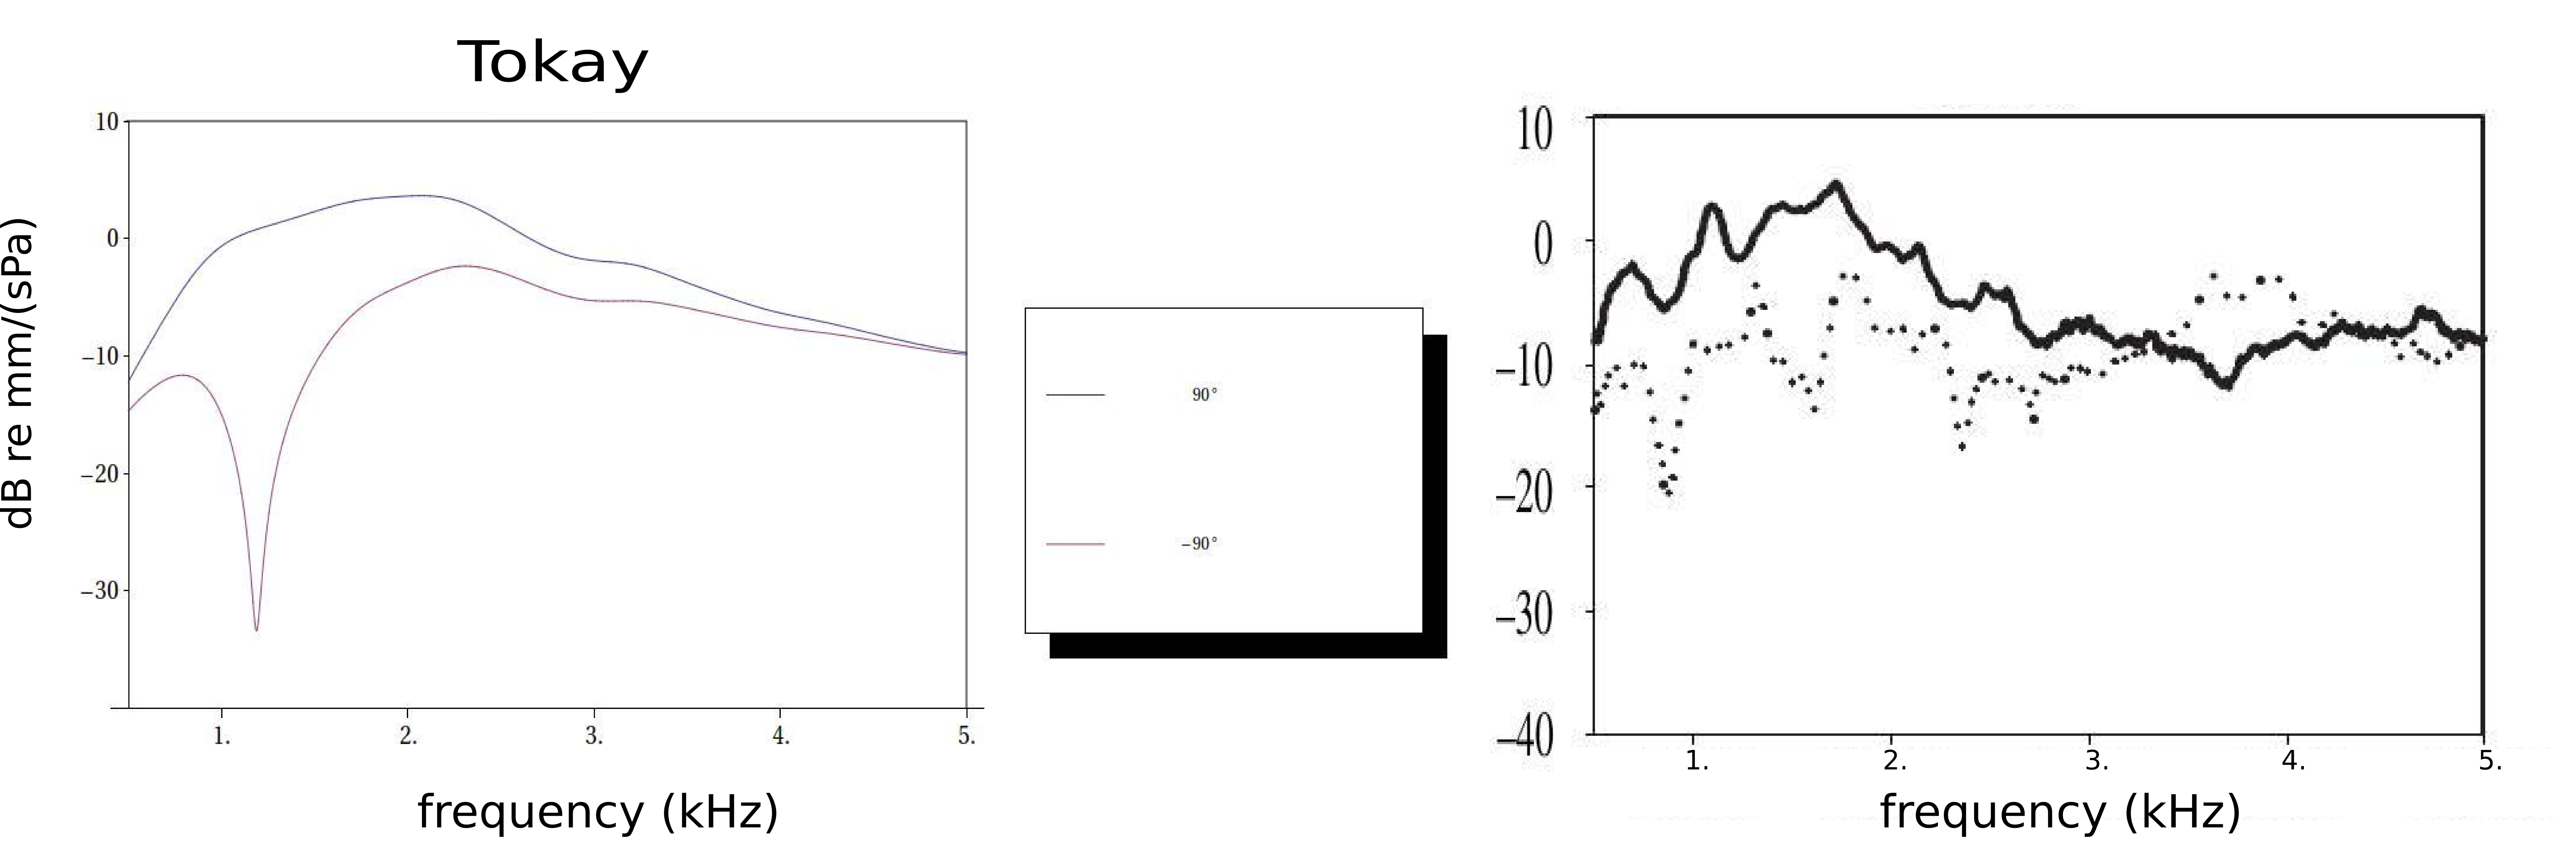
\includegraphics[width=1.0\linewidth]{Diagrams/Plots/tokayipsivscontrafull.png}
 \caption[Frequency dependence of ipsi- and contralateral membrane vibration amplitudes - Tokay gecko]{Calculated (left) and experimental (right) vibration velocity spectra for the Tokay gecko. In
 the plot on the right hand side, the thick line corresponds to an ipsilateral stimulus and the dotted line to a contralateral stimulus.  Data from \cite{dalsgaardmanley1}.}
  \label{tokayipsivscontrafull}
\end{figure}
\begin{figure}[ht!]
 \centering
  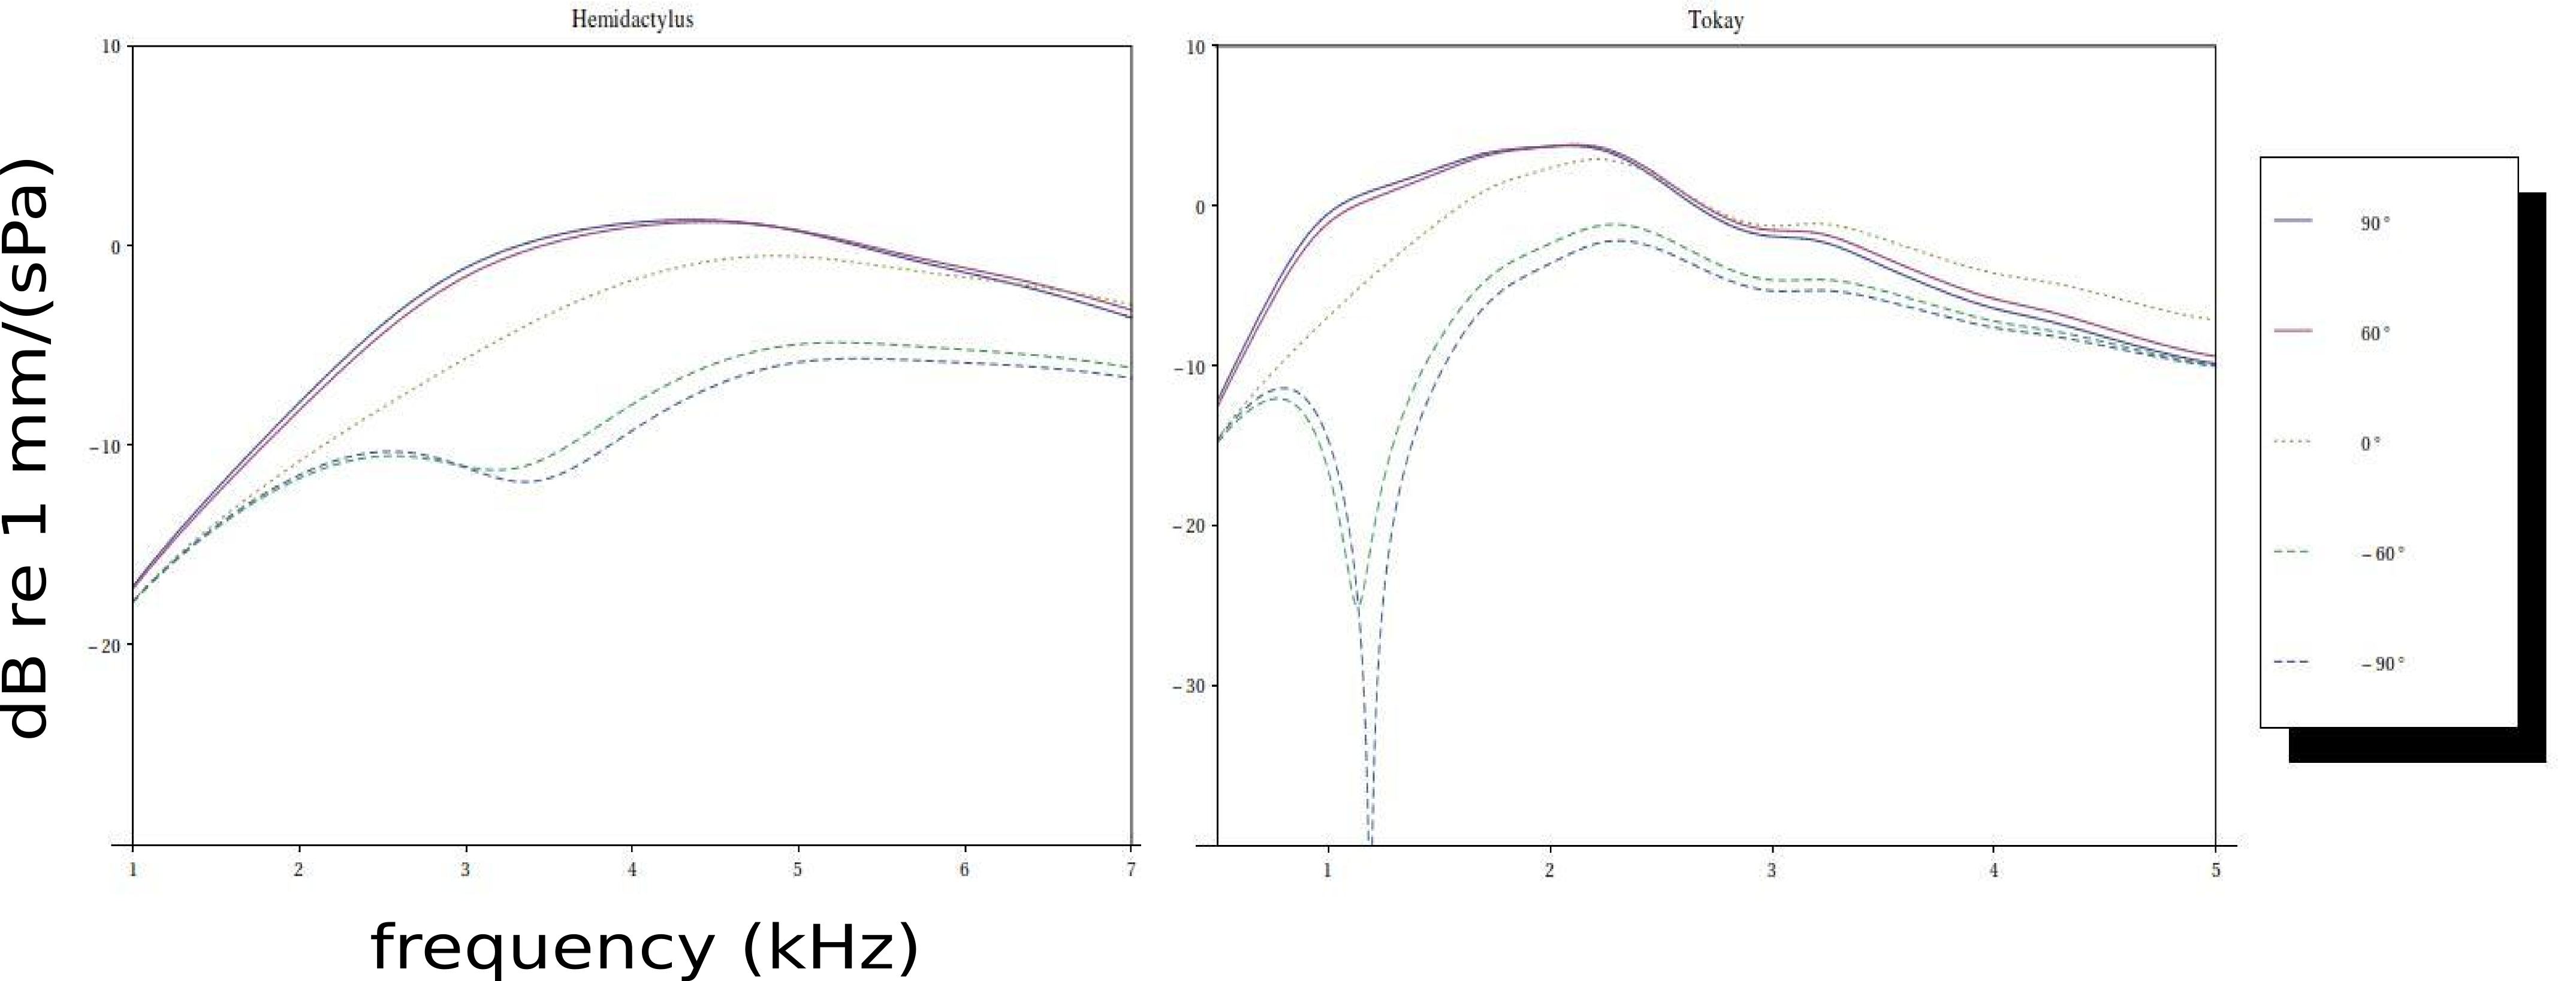
\includegraphics[width=1.15\linewidth]{Diagrams/Plots/freqdepboth.png}
  \caption[Frequency dependence of membrane vibration amplitudes for different directions.]{Frequency dependence of membrane vibration amplitudes for different directions - common house gecko (left), Tokay gecko (right). 
  The amplitude response to ipsilateral stimuli is generally higher and is at a maximum when the object is nearest to the ear i.e. $\theta=90^\circ$. The dotted line denotes a sound source directly in front of or behind the animal and the dashed lines denote contralateral stimuli.}
  \label{freqdepboth}
\end{figure}

We conclude this section by looking at the directional dependence of the vibration for a given set of frequencies. In Fig. \ref{directionplots}, we show the variation of the vibration amplitude of the membrane as
the sound source moves around the animal i.e. as $\theta$ varies from $-180^\circ$ to $180^\circ$.
\begin{figure}[ht!]
\centering
  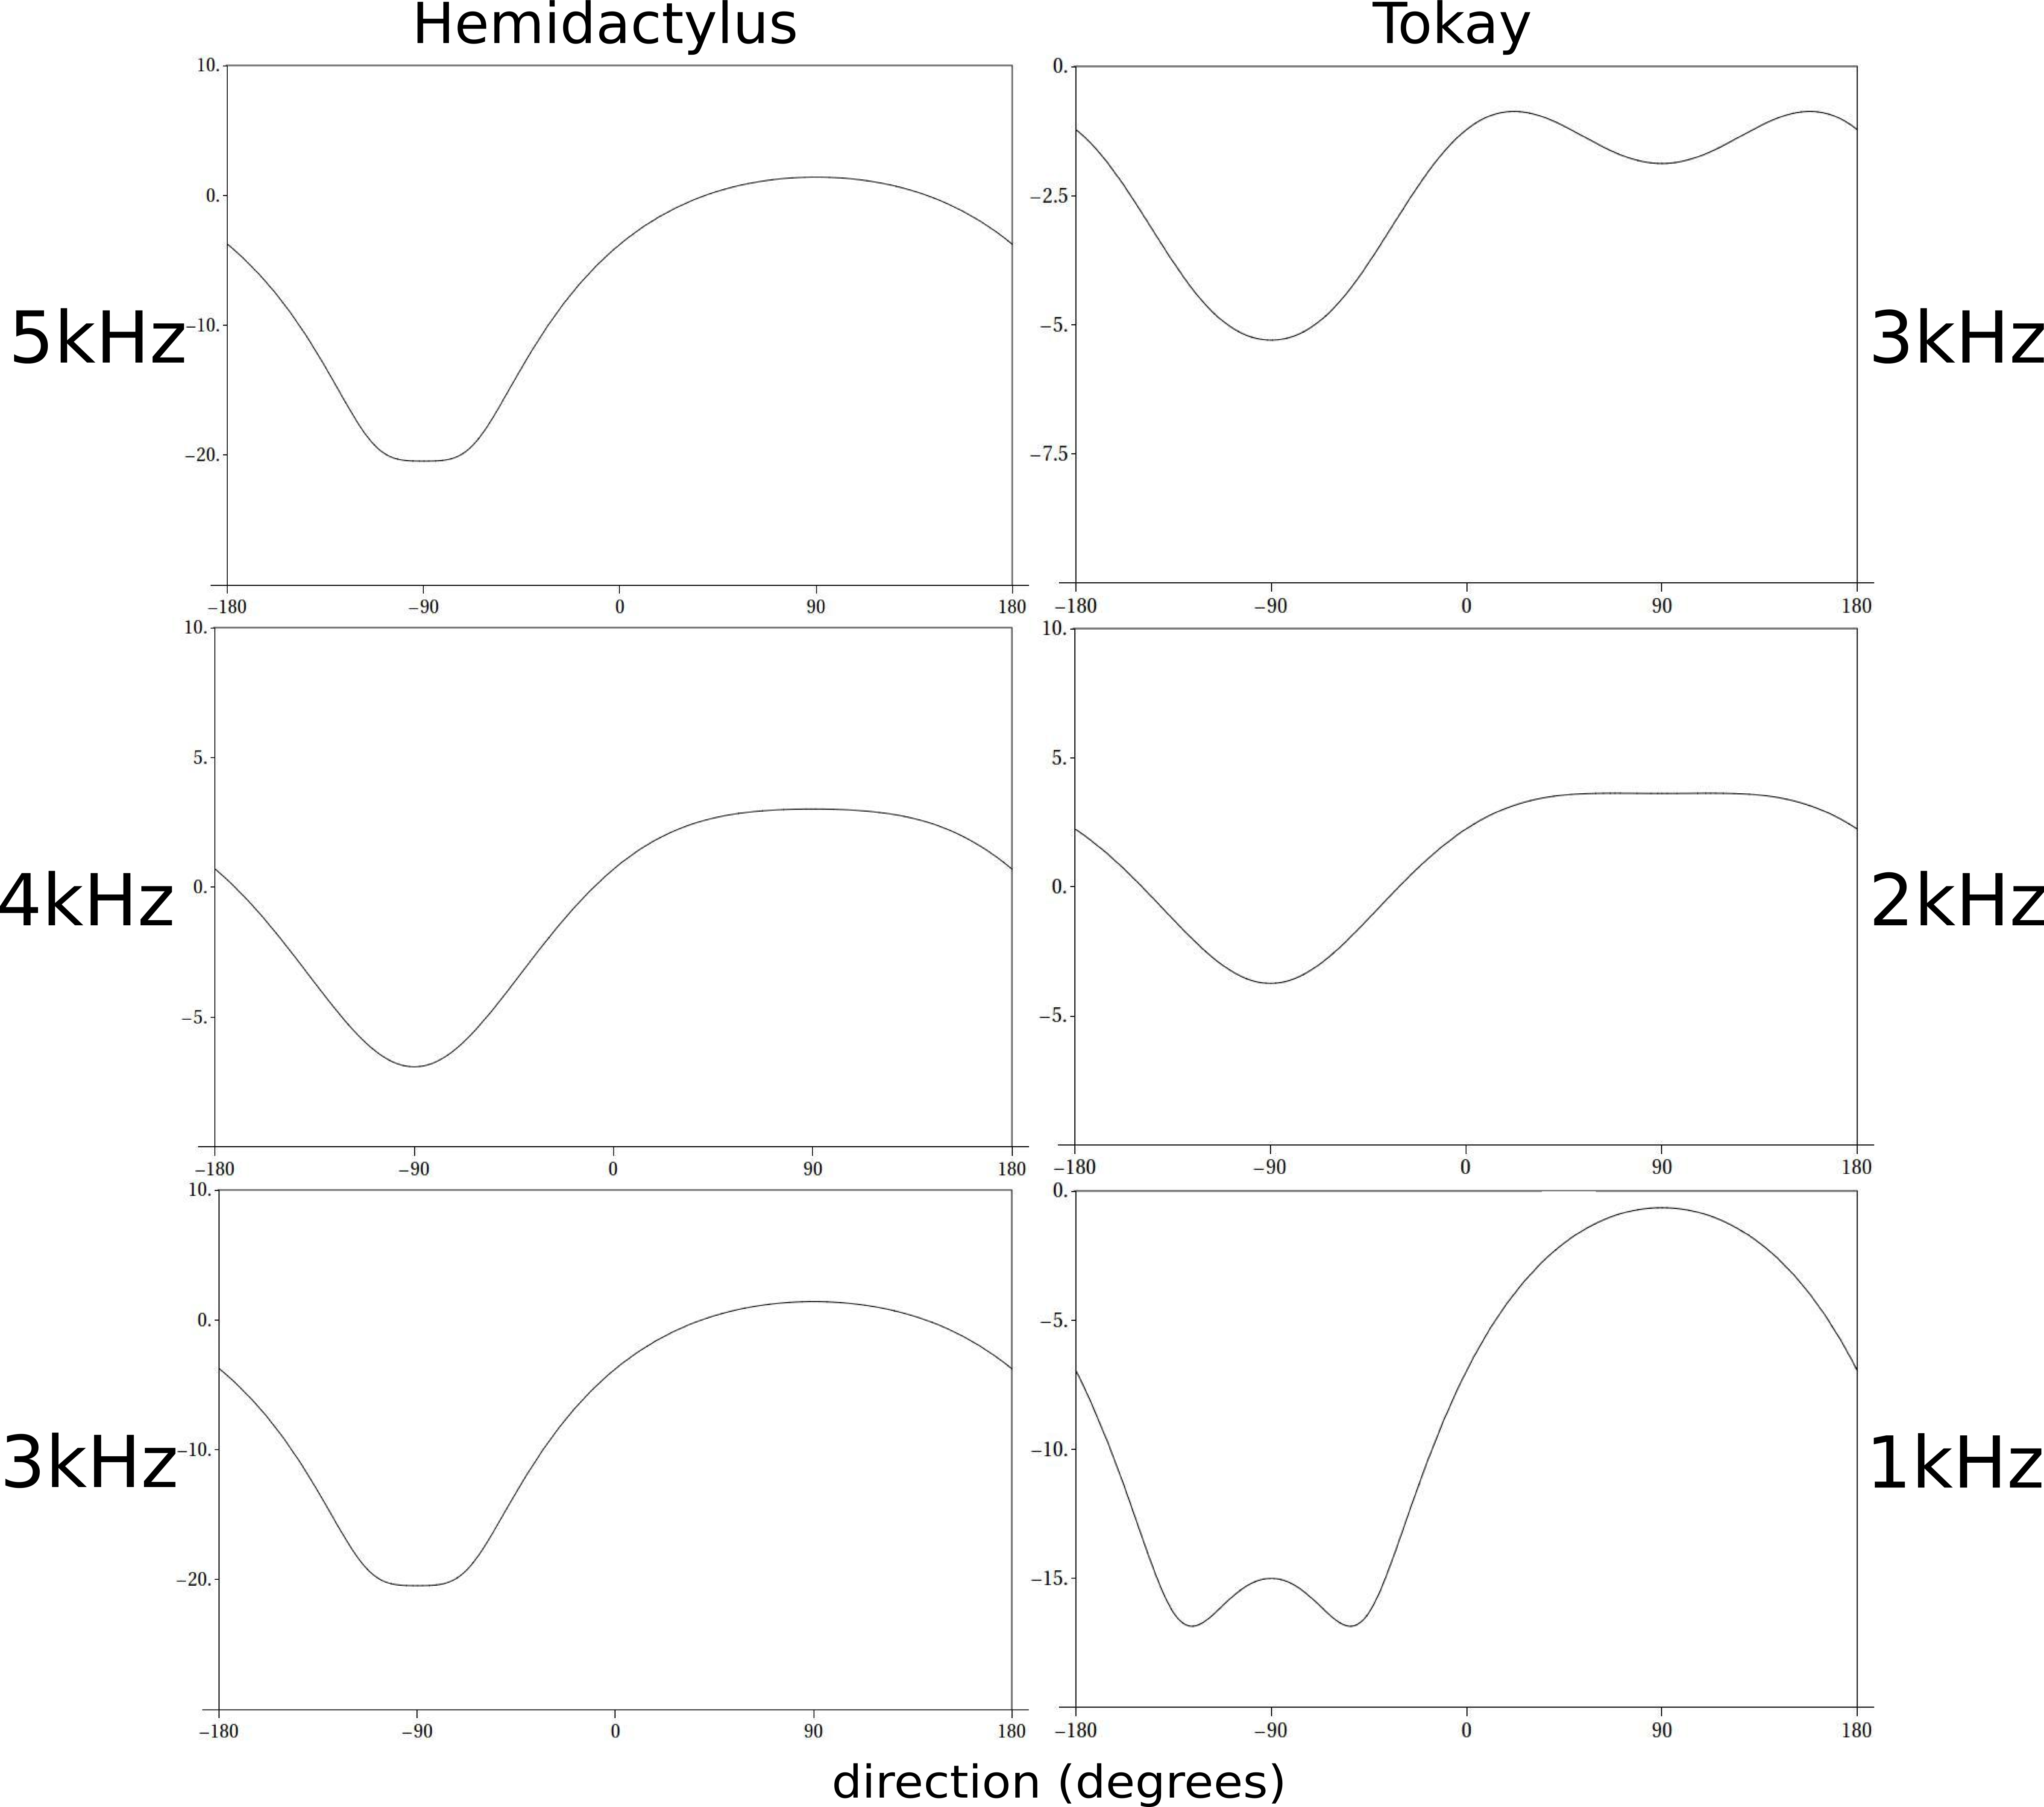
\includegraphics[width=.75\linewidth]{Diagrams/Plots/directionplots/directionplots.png}
  \caption[Direction dependence of membrane vibration amplitudes for different frequencies.]{Direction dependence of membrane vibration amplitudes  in the ICE Model for different frequencies - common house gecko (left, at 3kHz, 4kHz and 5kHz)
  , Tokay gecko (right, at 1kHz, 2kHz and 3kHz).
  The variation of the amplitude as the sound source completes a full circle around the animal is illustrated. The amplitudes for ipsilateral stimuli are shown to be
  higher than those for contraletaral stimuli.}
  \label{directionplots}
\end{figure}
Here we can more clearly see that the amplitudes due to ipsilateral stimuli are higher than those due to contralateral stimuli. The marked asymmetry and the steepness across the midline (i.e. at $0^\circ$)
is also consistent with observations (\cite{dalsgaardmanley1}, \cite{dalsgaardmanley2}). The choice of our frequencies has to do with the typical hearing ranges of the geckos. The smaller house
gecko is most sensitive at higher frequencies (~3kHz) and the larger Tokay gecko at lower frequencies (~1kHz).

\subsection{Directional Hearing Cues}\label{hearingcuessection}
The significance of our results up to this point should
already be apparent. Due to the relatively small head sizes of the geckos, the sound arriving at the two ears differ very slightly in phase and not at all in amplitude. On the other hand
 these animals overcome the problem and create strongly directional membrane vibration amplitudes through the use of coupled ears. From
 form of the direction dependence of the membrane vibration amplitudes we see that individual amplitudes don't necessarily vary much with direction. In other words, although
 there is a clear difference between the ipsilateral and contralateral response, the difference between a given pair of ipsi- or contralateral directions (eg. between $90^\circ$
 and $75^\circ$ or between $-90^\circ$ and $-70^\circ$) isn't very significant. Moreover, for some frequencies it seems that the vibration amplitude is lower at $\theta=90^\circ$ 
 than at $\theta\sim 60^\circ$.
 As a result of this, the vibration amplitudes of the ears cannot be independently used to localize the objects. In order to do so by using the tympanic membrane 
 vibration amplitudes, we need to compare the variation of their differences with respect to direction.
We therefore need functions that accurately quantify the directional dependence of the system at a given frequency. 

%\newcommand{\defeq}{\vcentcolon=}
As a first step we define the two quantities that are the main focus of this chapter - the internal level difference (iLD) and internal time difference (iTD)
in terms of the total membrane velocities. 
\begin{align}
  \mbox{iLD}&\vcentcolon= 20\mbox{Log}_{10}\left(\left|\frac{\dot{S}^0}{\dot{S}^L}\right|\right)\label{iLDfirstdef}\\
  \mbox{iTD}&\vcentcolon= \mbox{Arg}\left(\frac{\dot{S}^0}{\dot{S}^L}\right)/\omega.\label{iTDfirstdef}
\end{align}
Due to the steady state approximation we have the added advantage that the ratio of the displacement amplitudes is equal
to that of the velocity amplitudes; see \eqref{membraness1}. The main advantage of the velocity amplitudes 
is their relative ease of measurement in experiments. The iLD measures the ratio between the amplitudes of the eardrums and is the same as the IVAD function defined by J\o{}rgensen \emph{et al}. \cite{jorgensenschmitz} and
is measured in dB. The iLD is positive for ipsilateral directions and negative for contralateral.
This agrees with observed behaviour and means that the response of the system is directional.  The iTD corresponds to the time
difference (or equivalently phase difference) between the membrane vibrations. The ipsilateral ear is always ahead in phase
with respect to the contralateral ear. This means that it is negative for ipsilateral directions and positive for contralateral.

The iTD and iLD can be seen as the output of the ICE system with $p_0$ and $p_L$ as inputs.
In contrast, the Interaural Time and Level Differences (ITD and ILD) are entirely determined 
by the inputs to the two ears. The ITD is defined as the time difference between the vibrations between the vibrations of
the eardrums in the absence of coupling. It is calculated from the phase difference between the inputs at both ears;see \eqref{oldsoundinput}
\begin{equation}
\mbox{ITD}=\frac{Arg(pL/p0)}{\omega}=1.5\frac{L}{c}
\end{equation}
Due to the 
input pressures having the same amplitude and due to the linearity of the system (w.r.t sound input), in the absence of coupling the membranes
of the ICE model cannot have any a priori Interaural Level Difference. In larger animals
like humans the difference between the input amplitudes increases with frequency due to 
diffraction effects (shadowing) which aids in localization; cf. \cite[p~.154]{fletcheracoustic}. In addition, the gain in ITD due
to their increased head size also provides sufficient information for localization at lower frequencies.

In order to effectively function as cues for localization the iLDs and iTDs should ideally satisfy the following requirements,
\begin{enumerate}
 \item \label{listitem1} For a significant frequency range, they should increase with the adjacency of the sound source and should reach their maximum at $\theta=90^\circ$ and
 their minimum at $\theta=-90^\circ$.
 \item \label{listitem2} The iTD in particular should remain more or less constant for a given frequency range thereby mirroring the behaviour
 of the ITD. As different sets of neurons are sensitive to different frequencies, a constant delay is advantageous from the point of view of neuronal processing
 (cf. Sec. \ref{iceneuro}). 
 This is equivalent to the requirement that the phase difference is
 directly proportional to the frequency (see \eqref{iTDfirstdef}.
  \item \label{listitem3} They should go to zero at $\theta=0^\circ \mbox{ and } \theta=\pm 180^\circ$ meaning they should vanish when the object is directly
 in front of and behind the animal.
\end{enumerate}
The last of these requirements is ensured by the symmetry of our system as $p_0=p_L$ at $\theta=0^\circ \mbox{ and } \pm 180^\circ$ .
The first and second, on the other hand are more subtle aren't necessarily satisfied for all systems but as we will subsequently see, with our choice of
parameters they will be to a great degree. 

\subsubsection{Internal Level Differences}
In Fig. \ref{hemidactylusilDboth} (house gecko) and Fig. \ref{tokayilDboth}, we plot the
variation of the iLD with direction and frequency. The conventions for the $x-$ and $y$-axes remain the same as the ones in Figures \ref{hemidactylusvibampfull}
and \ref{tokayvibampfull}. The iLDs vary systematically with frequencies and peaks at around $3$kHz for the house gecko and around $1$kHz for the Tokay gecko.
As expected, they are positive for ipsilateral directions and negative for contralateral. The contour plots serve the purpose of giving us the simultaneous frequency and direction dependence of the iLDs well but the 
satisfaction of requirement \ref{listitem1} given in the above list isn't automatically clear.
\begin{figure}[ht!]
 \centering
 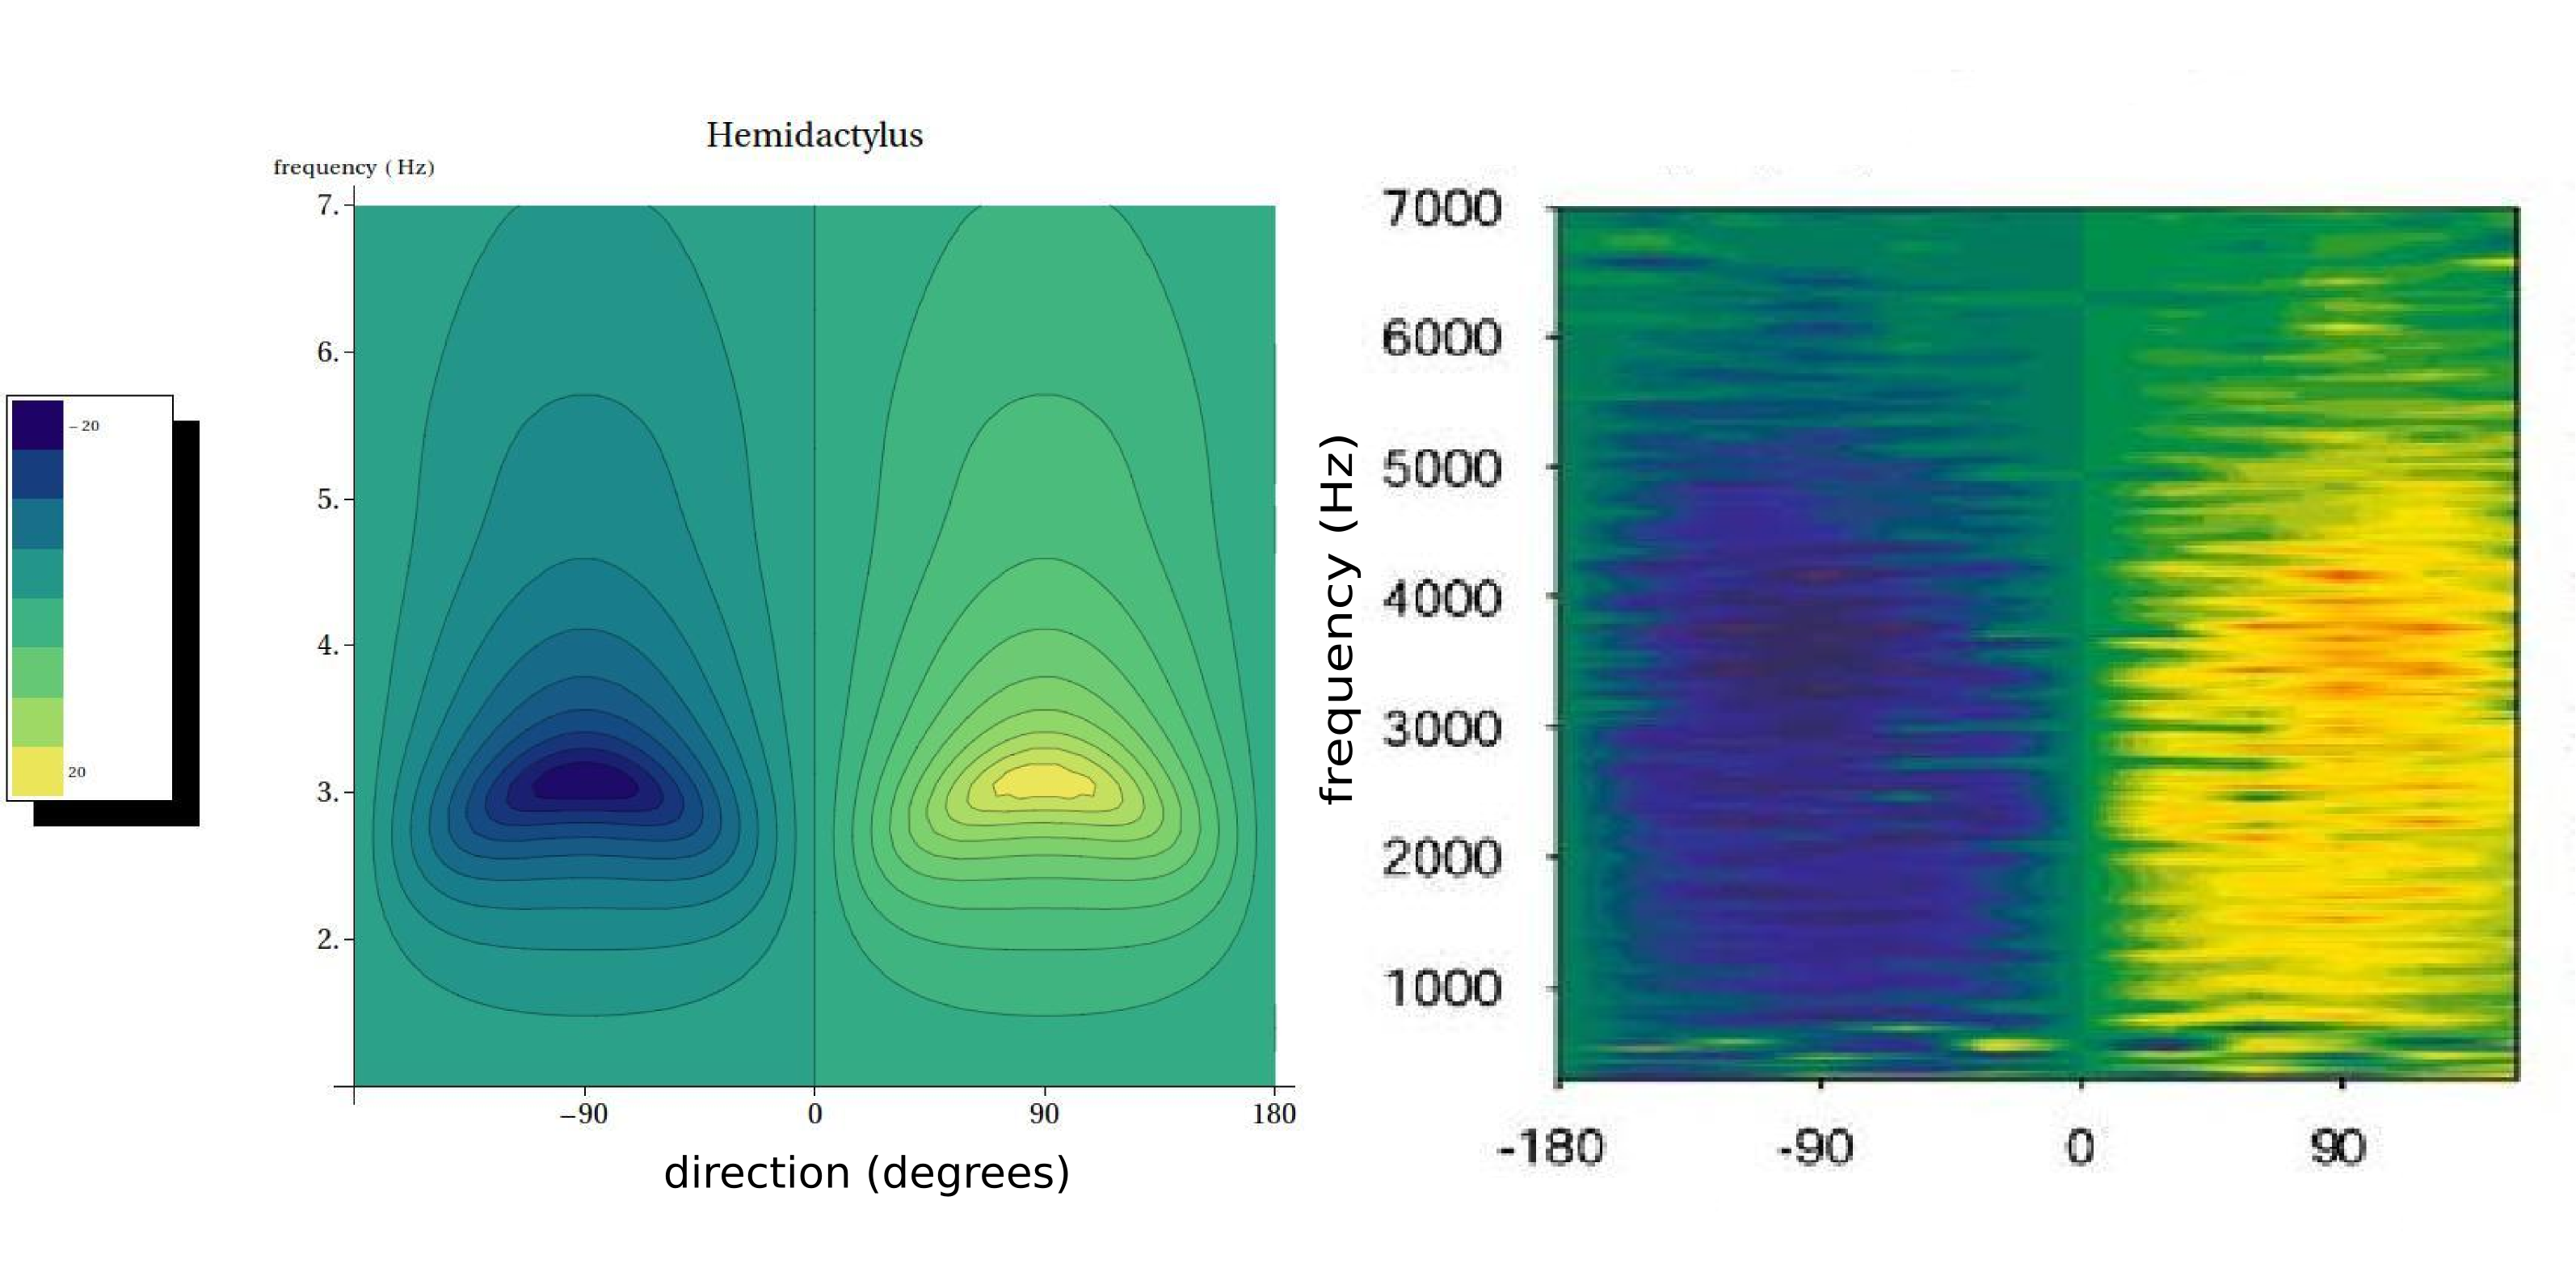
\includegraphics[width=1.0\linewidth]{Diagrams/Plots/iLD/hemidactylusiLDboth.png}
 \caption[ILD plots for the common house gecko]{Calculated (left) and experimental (right) Internal Level Difference of tympanic membrane vibrations for the common house gecko
 in dB. $x$-axis denotes direction in degrees (negative angles contralateral, 0 frontal and positive angles ipsilateral and the $y$-axis frequency in kHz. 
 Calculated and experimental values \cite{dalsgaardmanley2} show similar qualitative behaviour. See also Fig. \ref{tokayilDboth}.}
  \label{hemidactylusilDboth}
\end{figure}

\begin{figure}[ht!]
 \centering
 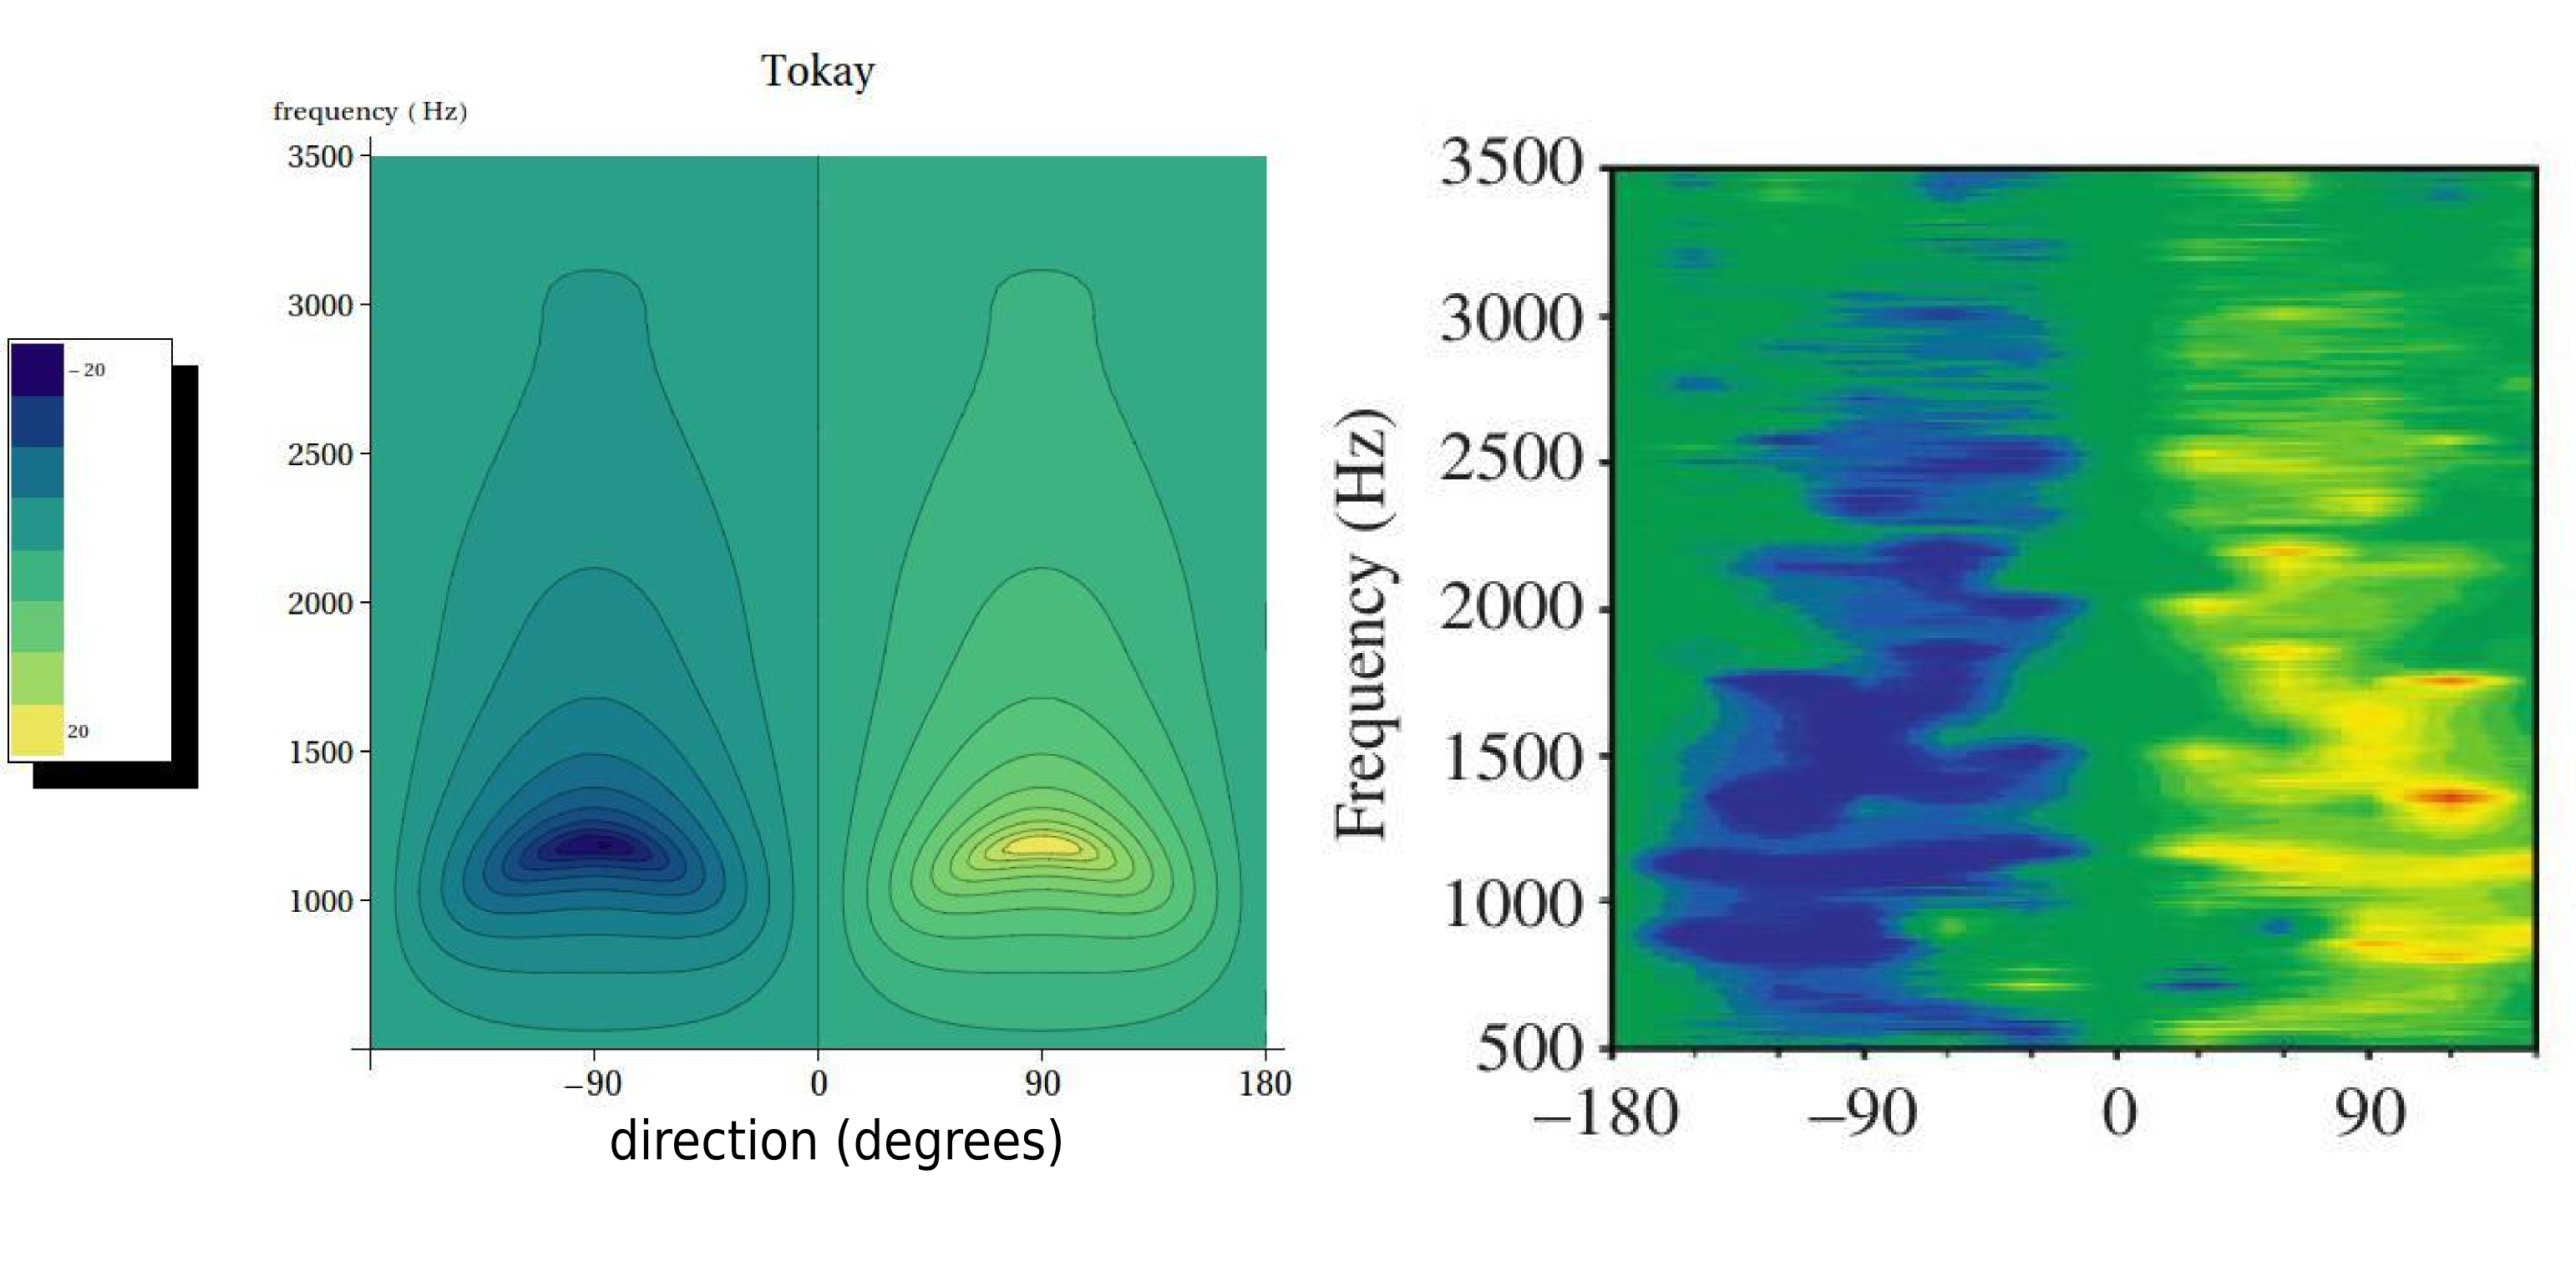
\includegraphics[width=1.0\linewidth]{Diagrams/Plots/iLD/tokayiLDboth.png}
 \caption[ILD plots for the Tokay gecko]{Calculated (left) and experimental (right) Internal Level Difference of tympanic membrane vibrations for the Tokay gecko
 in dB. The experimental values are taken from Christensen-Dalsgaard \cite{dalsgaardmanley1}.}
  \label{tokayilDboth}
\end{figure}

In order to better understand the direction dependence of iLD, we plot the variation
of iLDs with direction for a given set of frequencies in Fig. \ref{iLDdirection} (left:the house gecko, right:and Tokay gecko). We see that although the 
iLD has higher values below $3$kHz for the house gecko (below $1$kHz for the Tokay gecko), the form of the iLD for higher frequencies reflects the sinusoidal input better by peaking at fully
ipsilateral and contralateral directions. This suggests that iLDs may work better as directional cues at higher frequencies. In Fig. \ref{iLDspectrum}
we see this behaviour more clearly. Here we have plotted the iLD for a stimulus at $\theta 90^\circ$ with respect to frequency for both species. The bandpass behaviour
is clearly shown - the house gecko has a maximum difference of $30$ dB at around 3kHz and the Tokay gecko iLD peaks at $36$dB at around 1kHz. Also indicated in the figure is the directional bandwidth
for both animals. This is defined as the frequency range in which the iLD for an ipsilateral stimulus differs by more than 3dB. For the house gecko this is around $4.9$kHz and for the Tokay gecko it is around
$2.6$kHz which is in very good agreement with experimentally observed values (\cite{dalsgaardmanley1}, \cite{dalsgaardmanley2}). The fact that the calculated iLDs
agree well with experimental values numerically suggests that the total membrane displacements are good measures of the membrane properties.
\begin{figure}[ht!]
\centering
  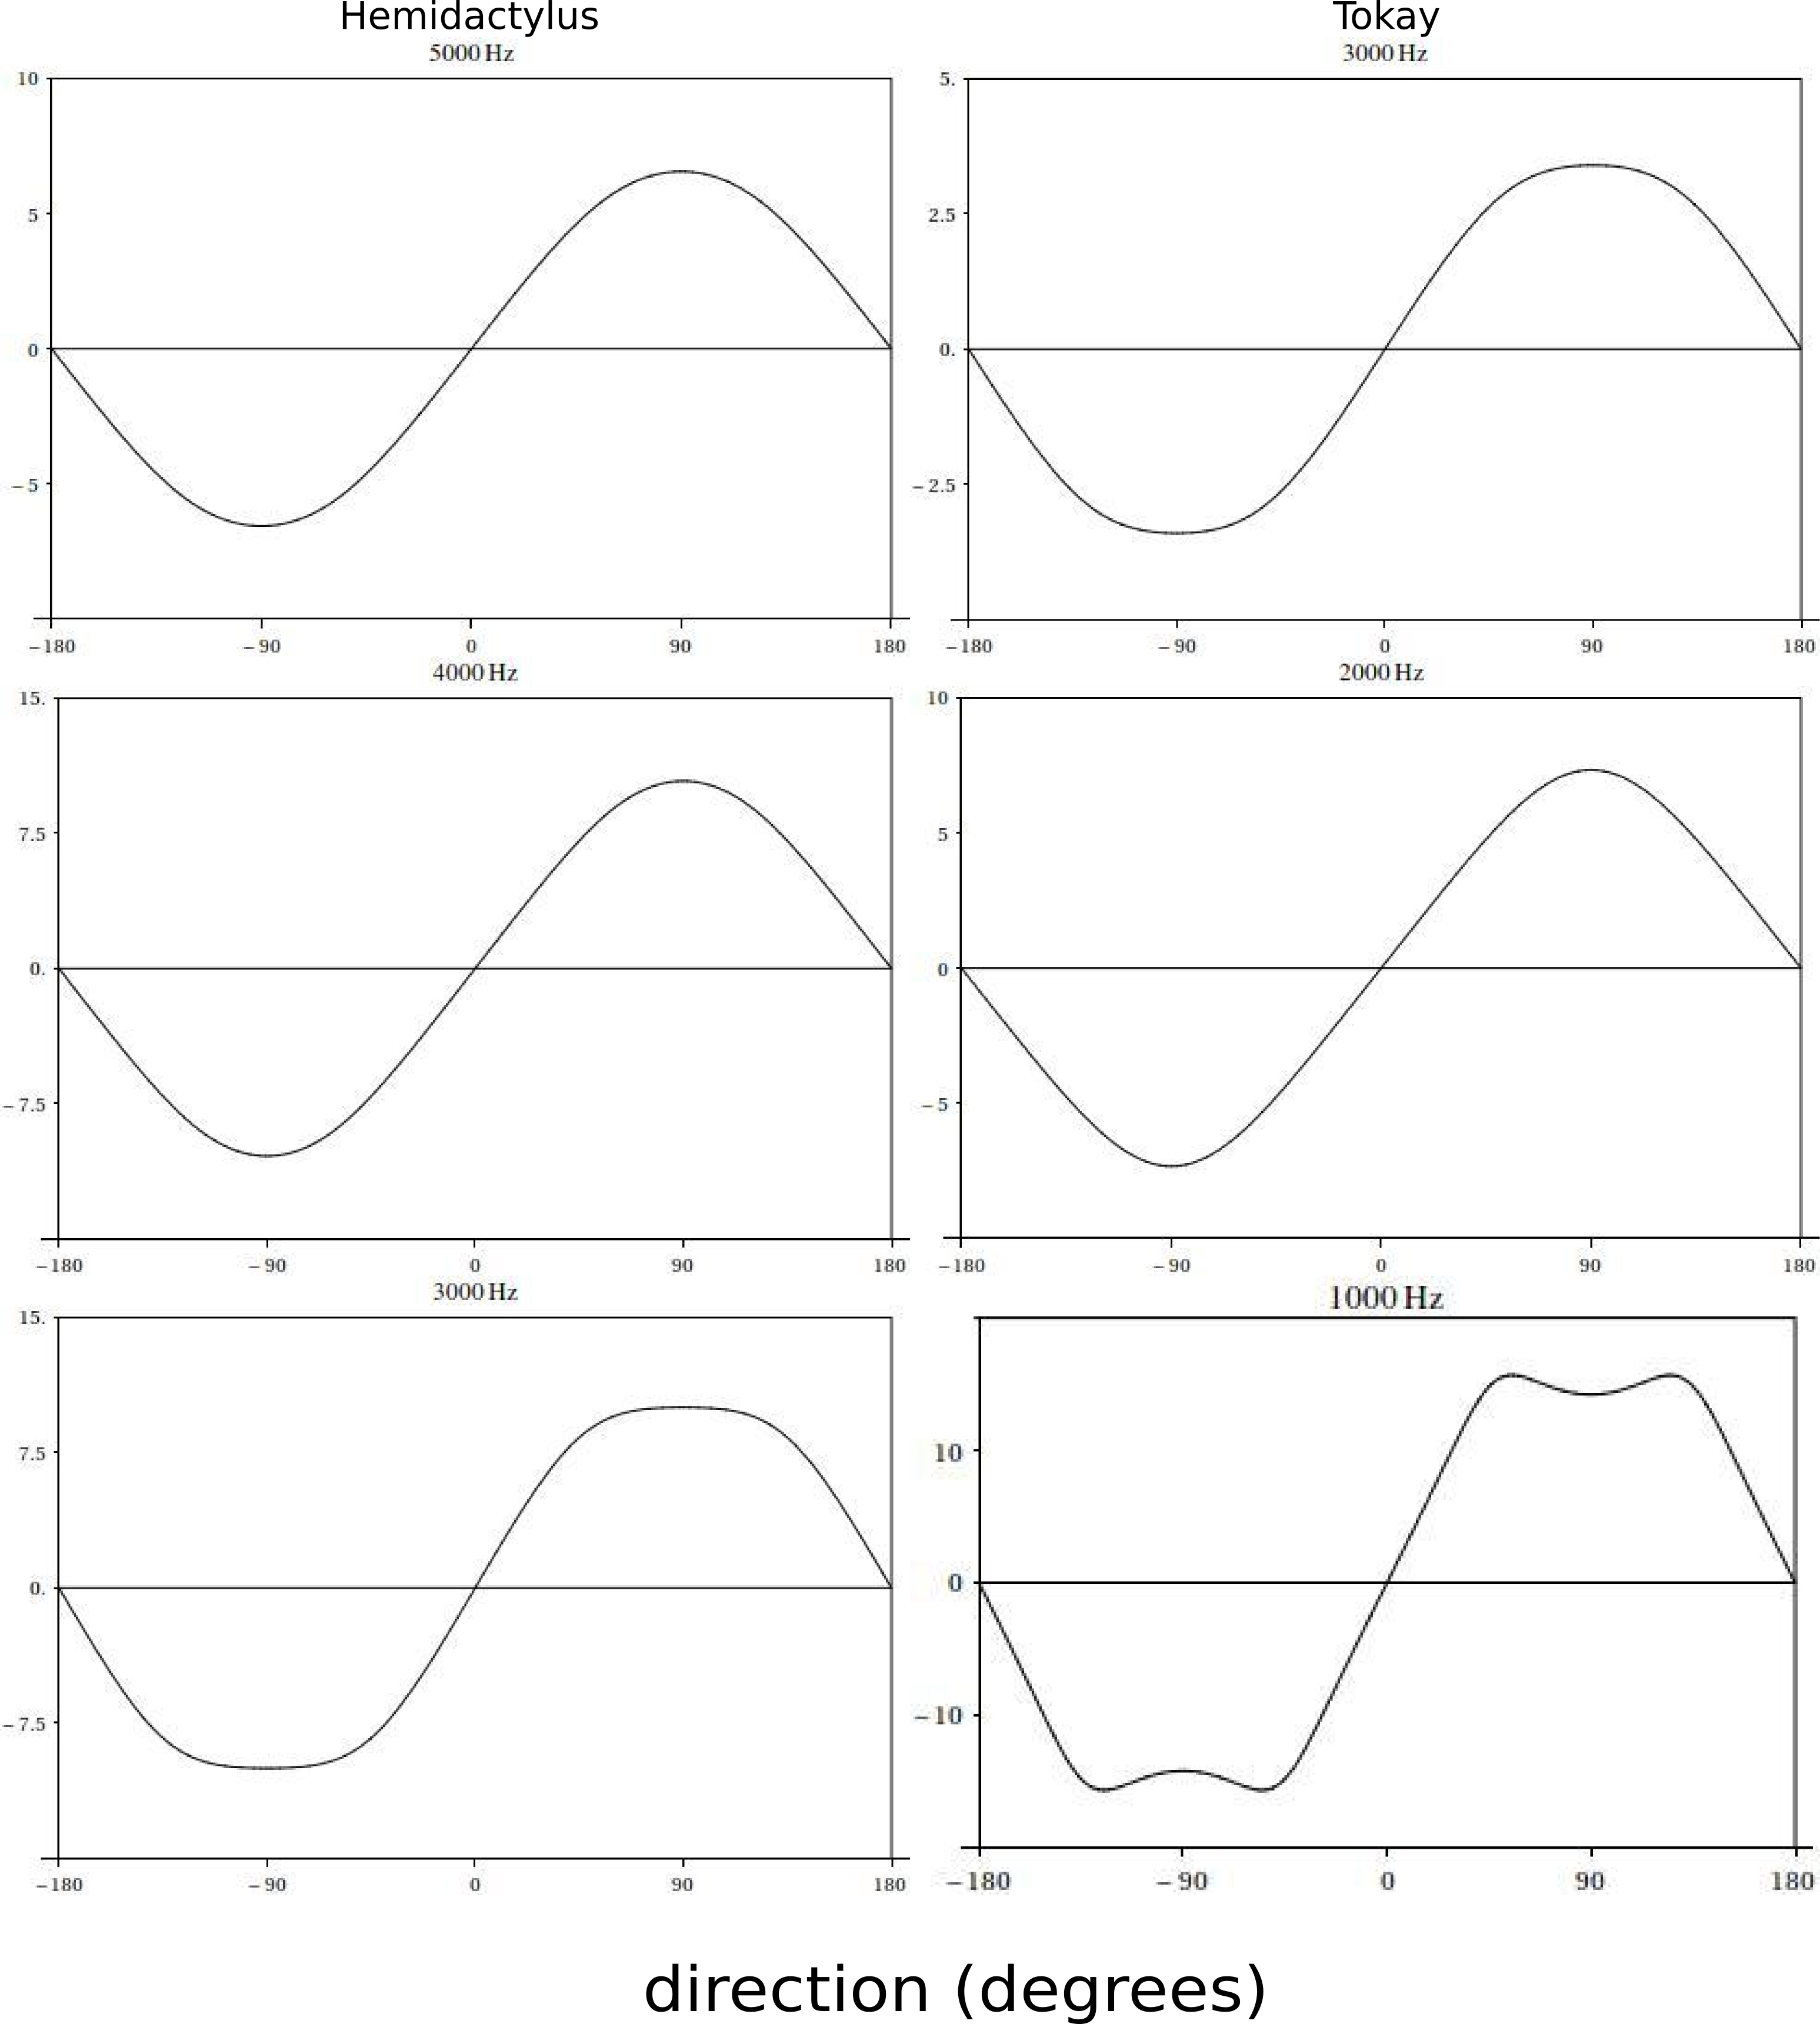
\includegraphics[width=.75\linewidth]{Diagrams/Plots/iLD/all.png}
  \caption[Direction dependence of the Interaural Level Difference for different frequencies.]{Direction dependence of the the Interaural Level Difference (cf. \eqref{iLDfirstdef}) in the ICE Model for different frequencies - common house gecko (left, at 3kHz, 4kHz and 5kHz)
  , Tokay gecko (right, at 1kHz, 2kHz and 3kHz). At higher frequencies, the iLD reaches a maximum at $90^\circ$ and a minimum at $-90^\circ$ whereas for lower frequencies, the maxima and minima are 
  reached before and after. This form of the above plots suggests that the iLDs cannot by themselves be used to localize sources in this regime and work better as directional cues at relatively higher frequencies.}
  \label{iLDdirection}
\end{figure}

\begin{figure}[ht!]
\centering
  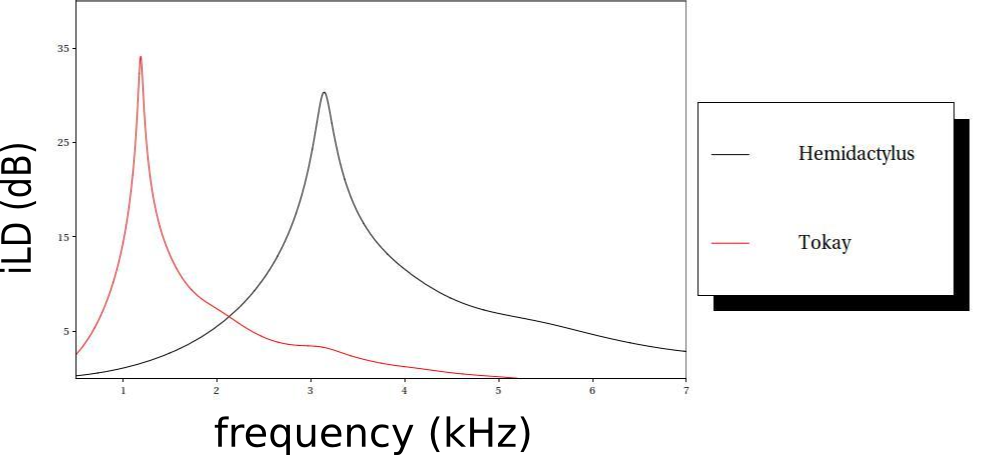
\includegraphics[width=.9\linewidth]{Diagrams/Plots/iLD/iLDspectrumboth2.png}
  \caption[Spectral behavior of the iLDs.]{Spectral behaviour of the iLDs at $\theta=90^\circ$ for the house gecko (black) and Tokay gecko (red). On the $x$-axis we have frequency in kHz and on the $y$-axis the iLD in decibels.
  The bandpass nature of the iLDs is clearly shown with a peaks at around $3$kHz for the house gecko and around $1$kHz for the Tokay gecko and is consistent with observations;\cite{dalsgaardmanley1}, \cite{dalsgaardmanley2}. The
  filled regions correspond to the directional bandwidth (frequencies at which iLD$>$3dB) of both animals. This value is around $4.9$kHz for the house gecko and $2.6$kHz
  for the Tokay gecko.}
  \label{iLDspectrum}
\end{figure}

\subsubsection{Internal Time Differences}
As we have just seen, the iLDs can be used as directional cues at relatively higher frequencies. The hearing range of geckos
on the other hand is found to contain lower frequencies as well. In Fig. \ref{iTDboth} we plot the variation of the iTD ($\mu$s; cf. \eqref{iTDfirstdef}) for 
a fully contralateral ($-90^\circ$) stimulus for both species with respect to frequency. From the figures we see that requirement \ref{listitem2} is satisfied fairly
well for both animals, albeit for different frequency ranges. At first, the lowpass behaviour as evidenced from the figure might seem counterintuitive as the
input phase differences vanish at zero frequency. But as the phase difference between the membranes increases more or less linearly for low frequencies,
a division by the angular frequency results in a constant value.

For the case of the house gecko, the ITD is around $43.7\mu$s and the resultant iTD between 
$500$Hz and $2.7$kHz has an iTD gain (the ratio of the iTD  w.r.t to the ITD)  of around three (or an iTD of around $123\mu$s). For the Tokay gecko, the ITD is around $96.2\mu$s which results in an iTD
gain of around $3.6$ (iTD of around $346\mu$s). These values stay more or less constant up to a certain frequency (around the first eigenfrequency of the membrane) and
sharply drop. As the frequency increases beyond this point, the iTD converges to the ITD. In Fig. \ref{itddirectionboth}, we plot the variation of the iTDs
with respect to direction for different frequencies. The frequencies are chosen to reflect the change in behaviour of the iTDs as it transitions from frequencies
below the first eigenfrequencies to those above. At frequencies below the first eigenfrequency (Tokay: $.5$kHz, $1$kHz, Hemidactylus: $1$kHz, $2$kHz) the iTDs
is significantly higher than it is at higher frequencies. At this point we should note that phase difference ceases to be useful as a directional cue when it is
greater than $2\pi$ or in other words when the iTD becomes greater than the time period at the given sound frequency ($1/f$). Thankfully, for the frequency ranges we are concerned with this will not be a problem.

\begin{figure}[ht!]
\centering
  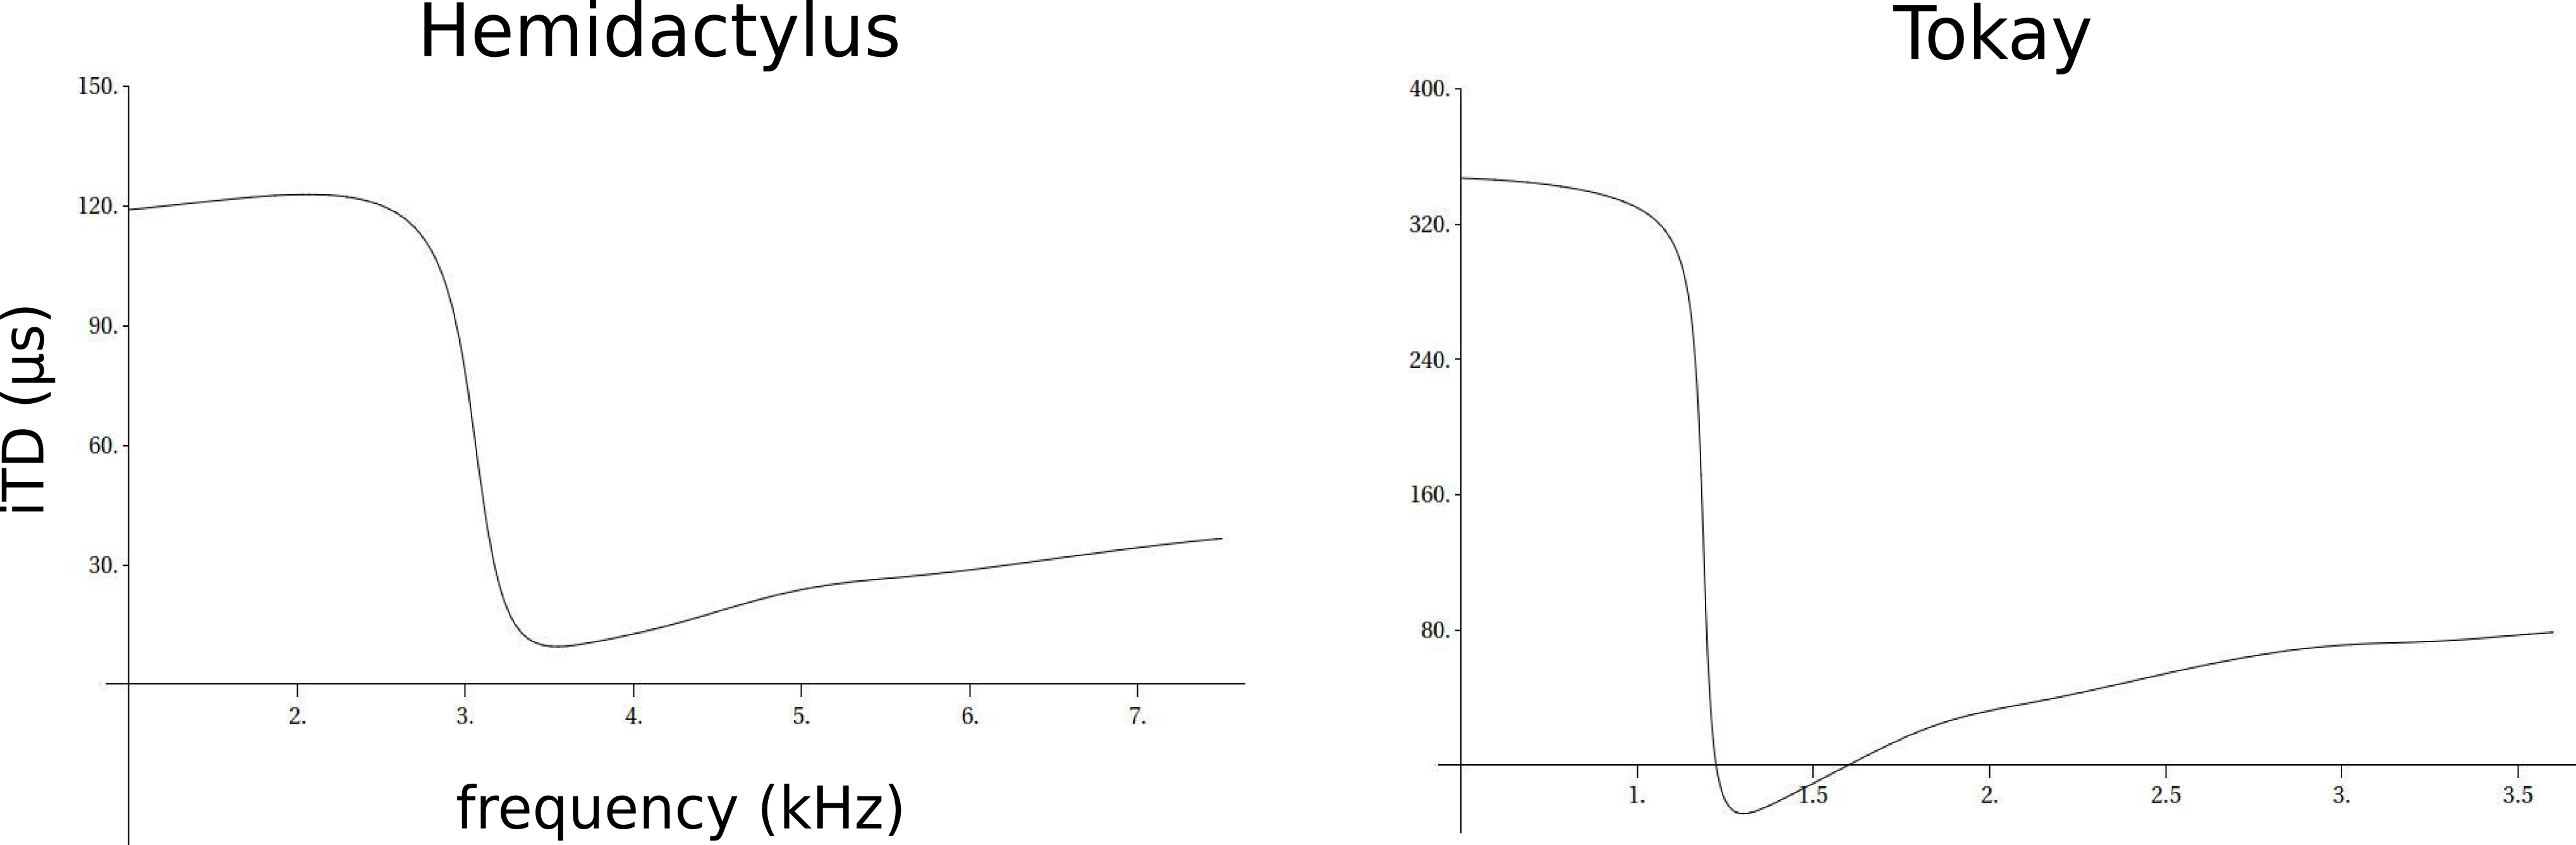
\includegraphics[width=1.0\linewidth]{Diagrams/Plots/iTD/both.png}
  \caption[Spectral behavior of the iTDs.]{Spectral behaviour of the iTDs at $\theta=90^\circ$ for the house gecko (black) and Tokay gecko (red). On the $x$-axis we have frequency in kHz and on the $y$-axis the iTD in $\mu$s.
  The bandpass nature of the iLDs is clearly shown with a peaks at around $3$kHz for the house gecko and around $1$kHz for the Tokay gecko as is consistent with observations;\cite{dalsgaardmanley1}, \cite{dalsgaardmanley2}.
  At frequencies above $f_0$ there is a sharp drop and iTD cues are no better than ITD cues. At these frequencies however, the iLDs are high enough to be used as directional cues.}
  \label{iTDboth}
\end{figure}

\begin{figure}[ht!]
%\centering
  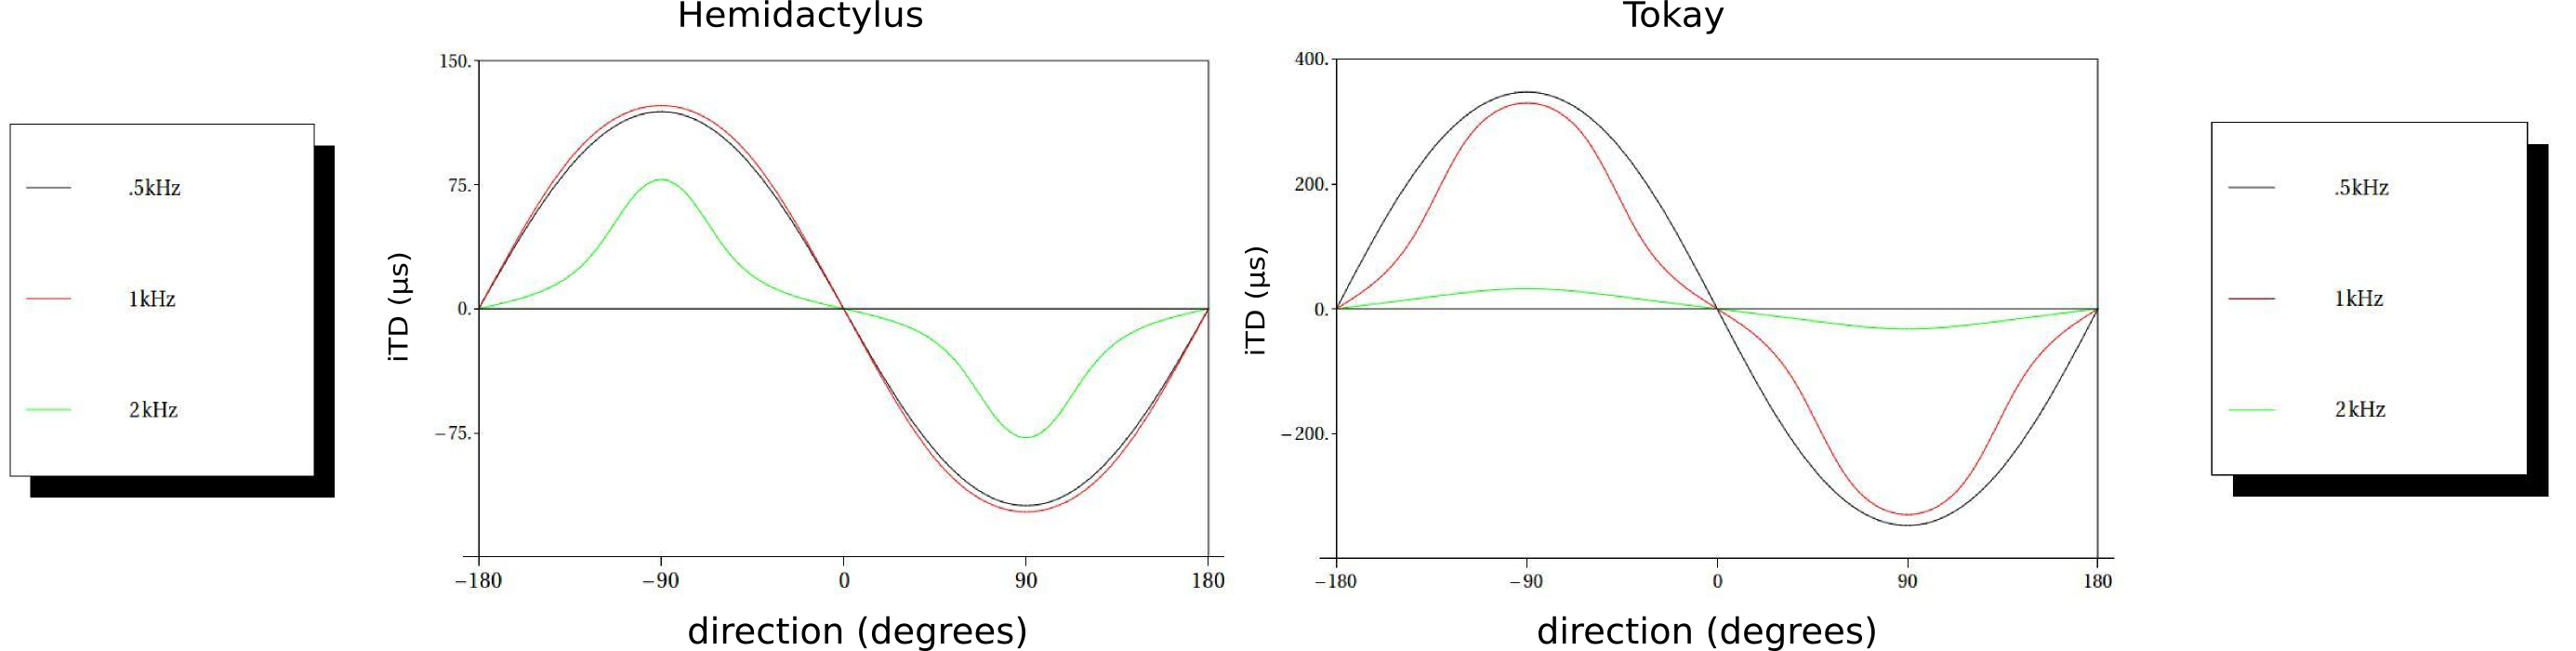
\includegraphics[width=1.0\linewidth]{Diagrams/Plots/iTD/itddirectionboth2.png}
  \caption[Variation of the iTD with direction for different frequencies.]{Variation of the iTD with direction for different frequencies. We can clearly see that the iTD cues are more pronounced
  at frequencies below $f_0$.}
  \label{itddirectionboth}
\end{figure}

\begin{figure}[ht!]
\centering
  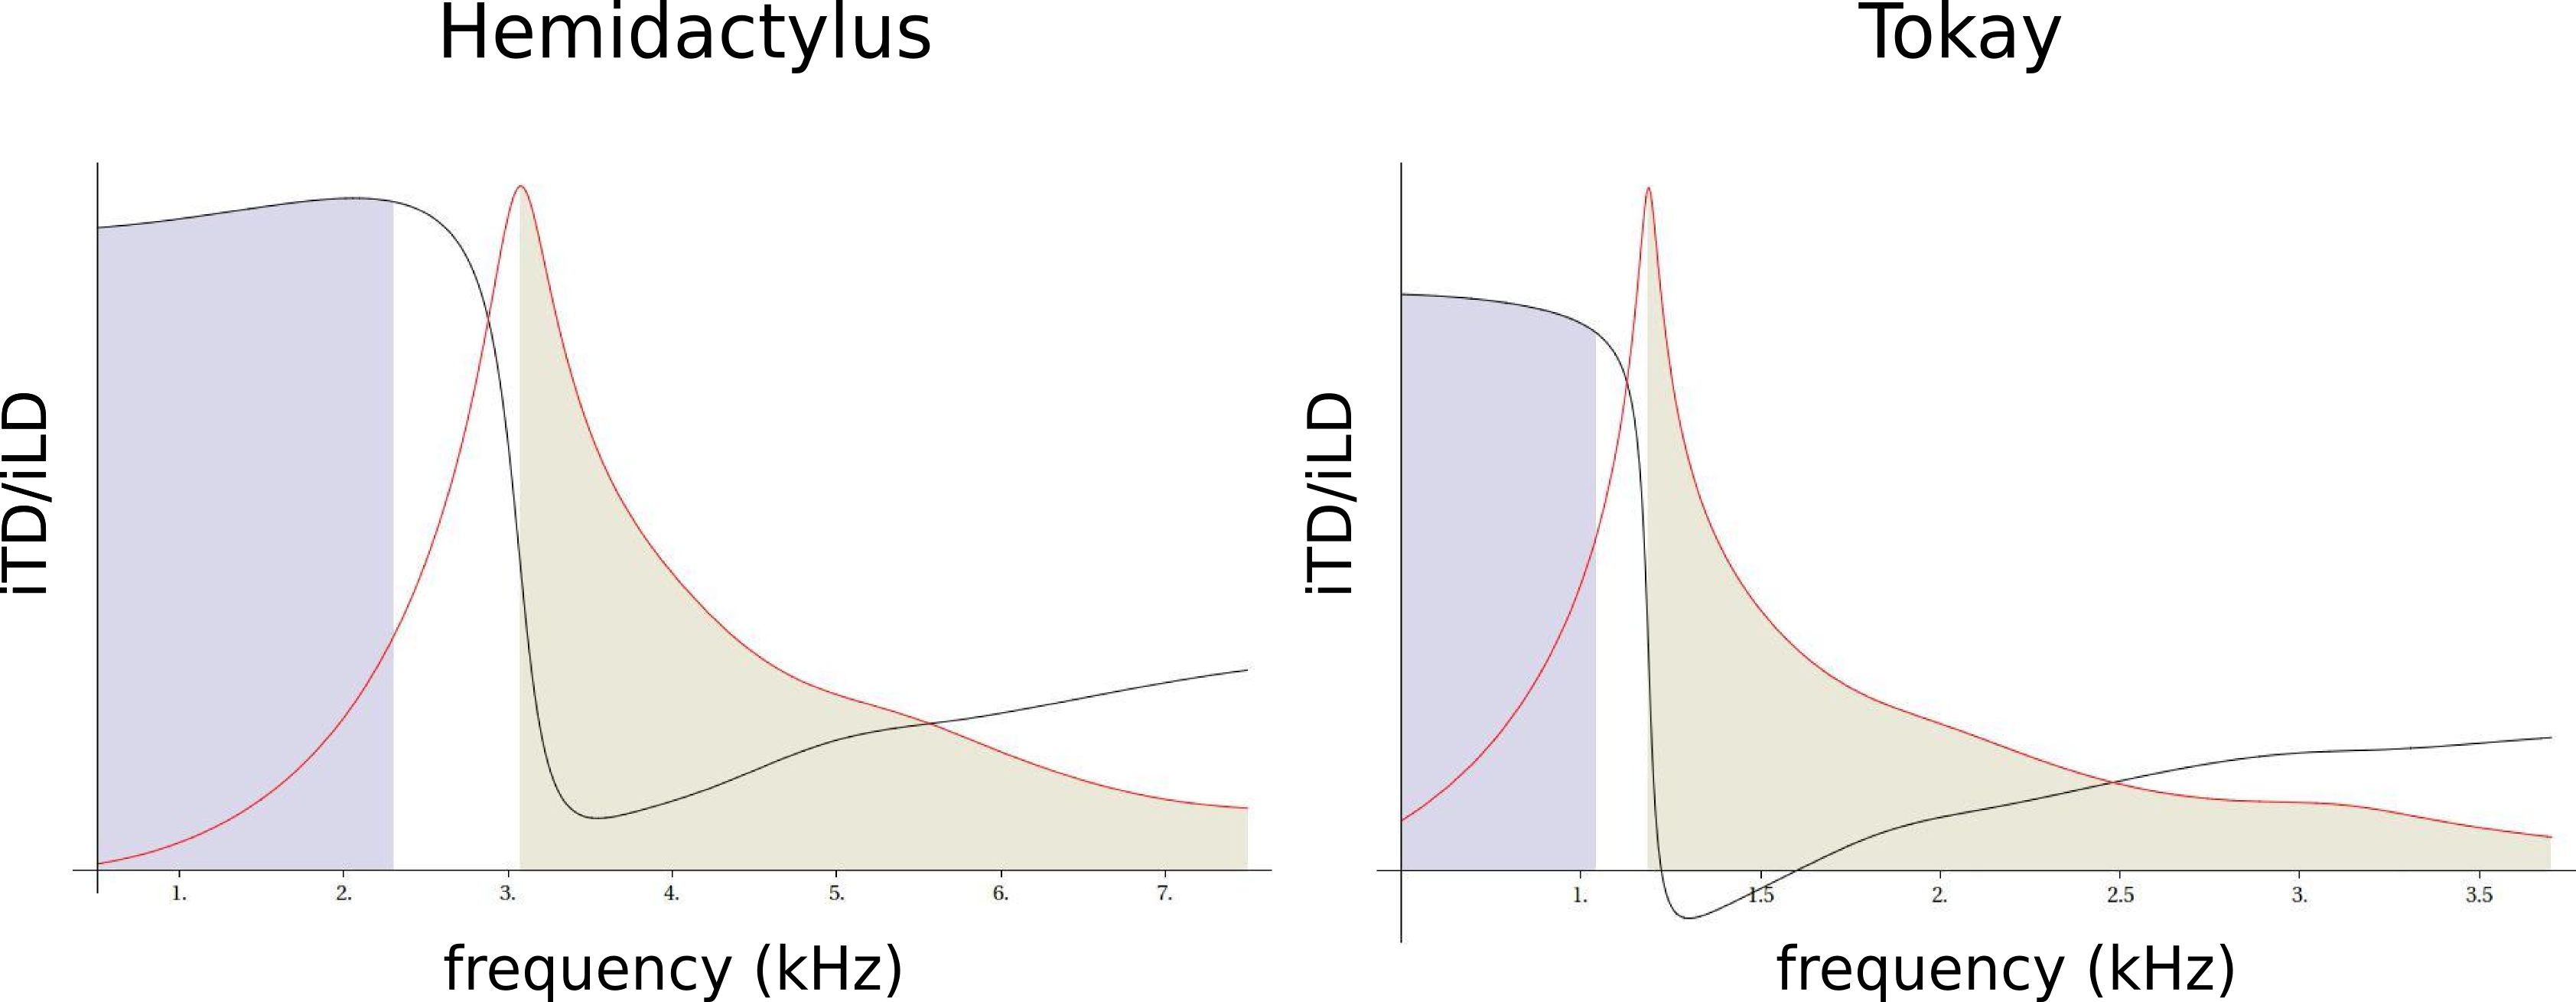
\includegraphics[width=1.\linewidth]{Diagrams/Plots/iTD/rangeboth.png}
  \caption[Possible frequency regimes for usage of iTD and iLD cues.]{ Possible regimes for the use of iTDs and iLDs for the house gecko (left) and Tokay gecko (right). The purple filled region corresponds to the iTD regime 
  and the beige filled region to the iLD regime. There is also a possibility of an overlap region where both cues can be used.  The iTD curves have been scaled to demonstrate the different
  regions more clearly.}
  \label{rangeboth}
\end{figure}

\subsubsection{}
The results up to this point tell us that just as in the case of animals with independent ears, animals
with coupled ears may find it more efficient to use time difference cues (iTDs) at lower frequencies and level difference
cues (iLDs) at higher frequencies. There might also be a frequency regime in which both cues can simultaneuously be used. In humans and
other mammals these cues arise due to the diffraction of sound around the animals head and body resulting in inputs on both ears with measurable
directional differences. Whereas in the ICE model, the only information about the direction of the sound source is in the form of a small phase
difference between the inputs to both ears. these difference arise from the coupling between the ears and the cutoffs are determined
by the system properties. 

In Fig. \ref{rangeboth} we simultaneously plot the iLD and iTD spectra in order to clearly demonstrate their regions of applicability. The first
region (purple) corresponds to the region where the iTD cues are more effective in ascertaining the direction of a sound source and the second
region (beige) to the region where an iLD based localization is more effective. There is an additional possibility of an overlap region where
both iTD and iLD cues can simultaneously be used.


% \subsubsection{Transmission Gain}
% 
% \subsubsection{Internal Time Difference}
% 
% \subsubsection{Internal Level Difference}

\subsection{Parameter Estimation}\label{parameterestimation}
Up to this point we have calculated the desired quantities in our model by using the values given in Table \ref{parametertable}.
Some of the parameters can be directly taken from their measured values whereas
the rest will need to be estimated indirectly. 
For the head width/interaural distance ($L$), cavity volume ($V_{\mathrm{\mathrm{cav}}}$), the density of the membrane ($\rho_m$)\footnote{A caveat: The density given in common models for the tympanum
is around $3$mg/mm$^3$ but this includes the mass of the transducer (the extracolumella). The density of the material of the tympanic membrane is in fact closer to the density of water,
hence the chosen value of $1$mg/mm$^3$} and its thickness ($d$)
we can use the directly measured values. The radius of the cylinder ($a_{cyl}$) can be calculated from the first two quantities
using \eqref{cylinderradiusformula}. 
As we've already seen in Fig. \ref{tympanummodel}, the realistic tympanic membrane is an ellipsoid rather than a perfect circle therefore the radius of our tympanum will
instead be estimated from the area of the membrane as $a_{\mathrm{tymp}}=\sqrt{A/\pi}$. For the extracolumella angle ($\beta$), we use the value estimated by Vossen \cite{vossenjasa}.

The parameters that require an indirect estimation are the first membrane eigenfrequency ($f_0$) and
its quality factor $Q$. The first of these effectively gives us the propagation speed of membrane vibrations, $c_M=2\pi f_0/\mu_{01}$ 
and the second gives us the membrane damping, $\alpha=\pi f_0/Q$. These quantities are difficult to directly measure and instead
have to be estimated from the frequency response of the system. In simulations of the ICE model, these parameters have been determined heuristically
while keeping the requirements \ref{listitem1}, \ref{listitem2} and \ref{listitem3} from page \pageref{listitem1} in mind. Nevertheless, for future work
it would be expedient to have a method to provide a rough estimate of these quantities from experimental results. In this way the calculation
of relevant parameters gives us an idea of their typical values for a given species.

A hint for their approximate values comes from the bandpass nature of the Internal Level Differences and the frequency at which the iLD maximum is attained.
This suggests that one of the membrane eigenmodes is dominant. In addition, as we have already seen, the iTDs remain constant for a significant frequency
range (\cite[p~.1996]{dalsgaardtangcarr}) putting further constraints on the value of $Q$. For the house gecko they have been experimentally is around $3$kHz and
 around $1.4$kHz for the Tokay gecko. Due to the complexity of the expression for the membrane vibration profile, the exact position of the iLD maximum is hard to directly calculate.

In order to better understand our parameter selection, we 
need to take a closer look at the analytical expression for the displacement ratio of the membranes and  simplify the expression after using the appropriate formulas for $G^s_{ipsi}$ and $G^s_{contra}$,
\begin{align}
 \frac{\dot{S}^0}{\dot{S}^L}&=\frac{\eta+e^{1.5jkL}}{1+\eta e^{1.5jkL}}\label{displacementratio}\\
 \mbox{where, }\eta&=\frac{G^s_{ipsi}}{G^s_{contra}}=\frac{\Lambda}{\rho c\omega}\sin kL-\cos kL.\nonumber
\end{align}
We have also set the direction of the source to be fully ipsilateral to the $x=0$ membrane, i.e. $90^\circ$. The complex frequency
dependence of the above term is entirely contained in the term $\eta$.

As stated towards the end
of Sec. \ref{coupledmembranes}, we have to choose an appropriate cutoff for the value of $\Lambda$. In general, this choice
depends on the values of $f_0$ and $Q$ and therefore on the hearing range of the animal. It is further complicated by
the fact that the corresponding zeros of the Bessel function $J_\kappa$ are very closely spaced. In our simulations up to this point
we have chosen an arbitrary cutoff of the first $30$ modes. A way around this difficulty can be found from the observation that the shape
of the iLD spectrum (see Fig. \ref{iLDspectrum}). It suggests that one of the membrane eigenmodes dominates in the expansion of $\Lambda$. 
For the purposes of an estimation 
we can therefore calculate $\Lambda$ up to the first eigenmode i.e. the $(1,1)$ mode (ref. Fig. \ref{sectoralmembraneeigenmodes} and \eqref{lamfirstdef}).
This gives us,
\begin{align}
 &\eta=G\widetilde{\Omega}_{01}\frac{\sin kL}{kL}-\cos kL\\
 &\mbox{where, }G=\frac{V_{\mathrm{\mathrm{cav}}}\rho_md}{\rho c^2 K_{01}}\nonumber.
\end{align}
The term $G$ contains all the information from the ``fixed'' parameters like cavity volume, membrane density, thickness etc. and
$\widetilde{\Omega}_{01}=(\omega^2-2j\alpha\omega-\omega^2_{01})$ contains the as yet unknown parameters, $f_0$ and $Q$. Substituting
this expression in \eqref{displacementratio} gives us the displacement ratio as a function of the frequency. 
We now find expressions for the iTD and iLD in terms of the above ratio,
\begin{align}
 &\mbox{ iLD }_{90}= 10\mbox{Log}_{10}\left(\frac{(\mbox{Re}(\eta)+\cos 1.5kL)^2+(\mbox{Im}(\eta)+\sin 1.5kL)^2}{(\mbox{Re}(\eta)+\cos 1.5kL)^2+(\mbox{Im}(\eta)-\sin 1.5kL)^2}\right)\label{iLDnewdef}\\
 &\tan\left(\omega\times\mbox{ iTD }_{90}\right)= \frac{(1-|\eta|^2)\sin 1.5kL}{\mbox{Re}(\eta)+(1+|\eta|^2)\cos 1.5kL}\label{iTDnewdef}
\end{align}
using \eqref{iLDfirstdef} and \eqref{iTDfirstdef}. We have used subscripts to indicate that the above terms have been calculated
at $\theta = 90^\circ$. We essentially have 
a expression for the iLD and iTD spectra with two unknown parameters. We now need two equations for a given frequency (or a given
pair of frequencies) that can be used to determine $Q$ and $f_0$. The first of these equations is obtained by requiring that
the derivative of the iLD goes to zero at a given frequency - $f_{\mathrm{max}}$, i.e. the experimentally determined frequency of 
peak amplitude difference.


The second equation requires us to put a constraint on the iTD. To do this we first look at the behaviour of the iTD for our system parameters for
different values of $Q$.
Qualitatively it can be said that the frequency of peak iLD is close to $f_0$ with exact position depending on $Q$ as well.
The dependence of the iTD on $Q$ is a little more complicated but perhaps more revealing. In Fig. \ref{itdQdependence}, we plot the variation of the 
iTD spectrum for the three typical ranges of $Q$. At ``low'' values of $Q$ the iTD increases up to a certain frequency and drops
 after reaching its maximum value, $1/f_0$. At higher values the iTD decreases steadily with frequency up to a certain value and
 somewhere in the middle, the iTD remains more or less constant up to a certain frequency. This behaviour gives evidence for the existence of an optimal value $Q_0$ 
for which the iTD  best satisfies requirement \ref{listitem2}. Due to the relation of the iTD to the complex argument, we can approximate this requirement by requiring that the second derivative of
the complex argument with respect to frequency vanishes at $f_0$.

\begin{figure}[ht!]
\centering
  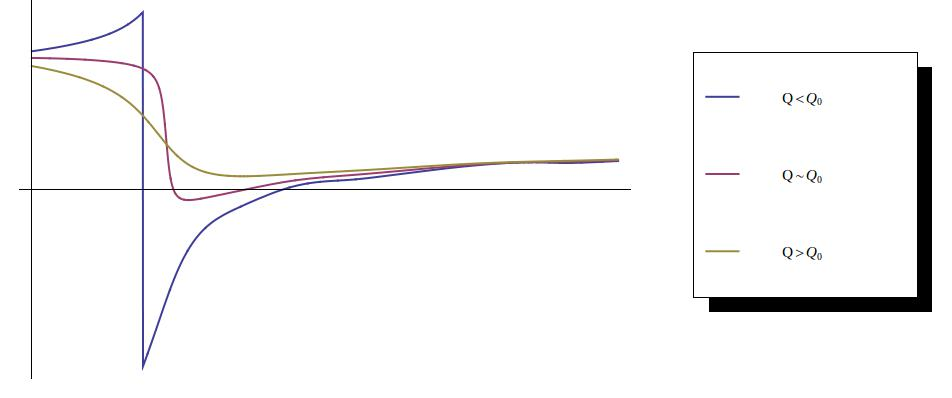
\includegraphics[width=.7\linewidth]{Diagrams/Plots/paramtest/allthree.jpeg}
  \caption[Dependence of iTD spectrum on Quality Factor]{The three curves correspond to the iTD spectrum for different values
  of Q. In the red curve we have the spectrum for a near ideal value of $Q$ such that the iTD remains more or less constant upto
  a given frequency. The blue curve corresponds to a low $Q$ for which the iTD increases upto a peak value ($1/f_0$) and drops afterwards.
  In the yellow curve we see that the iTD decreases steadily with frequency upto a certain point before converging to the ITD value.}
  \label{itdQdependence}
\end{figure}
\noindent These conditions can therefore be written as the following set of equations,
\begin{align}
 \left.\frac{d (\mbox{iLD}_{90})}{df}\right|_{f=f_{\mathrm{max}}}=0\\
 \left.\frac{d^2 \omega (\mbox{iTD}_{90})}{df^2}\right|_{f=f_{\mathrm{max}}}=0
\end{align}
These give us a pair of nonlinear equations that can be numerically solved to obtain values for $f_0$ and $Q$.

\section{Spatial Vibration Pattern of the Membrane}\label{vibrationpatternchapter}
We begin our analysis by evaluating the variation of the spatial vibration pattern of the tympanic membrane
with frequency. The tympanic vibration pattern was first measured experimentally by Manley \cite{manleygecko1}
for a \emph{Tokay gecko} and was found to have the strongest response at around 1kHz. The measured vibration patterns
are shown on the left in Fig. \ref{manleygeckotympanum}. Manley measured the vibration amplitude for eight locations on the membrane and measured the pattern
seen on the left of Fig. \ref{manleygeckotympanum}. As we can see, at around $4$kHz, the vibration pattern
distinctly develops two maxima - something that would not happen to a centrally loaded tympanum except
at frequencies well beyond the hearing range of geckos.
\begin{figure}[ht!]
 \centering
 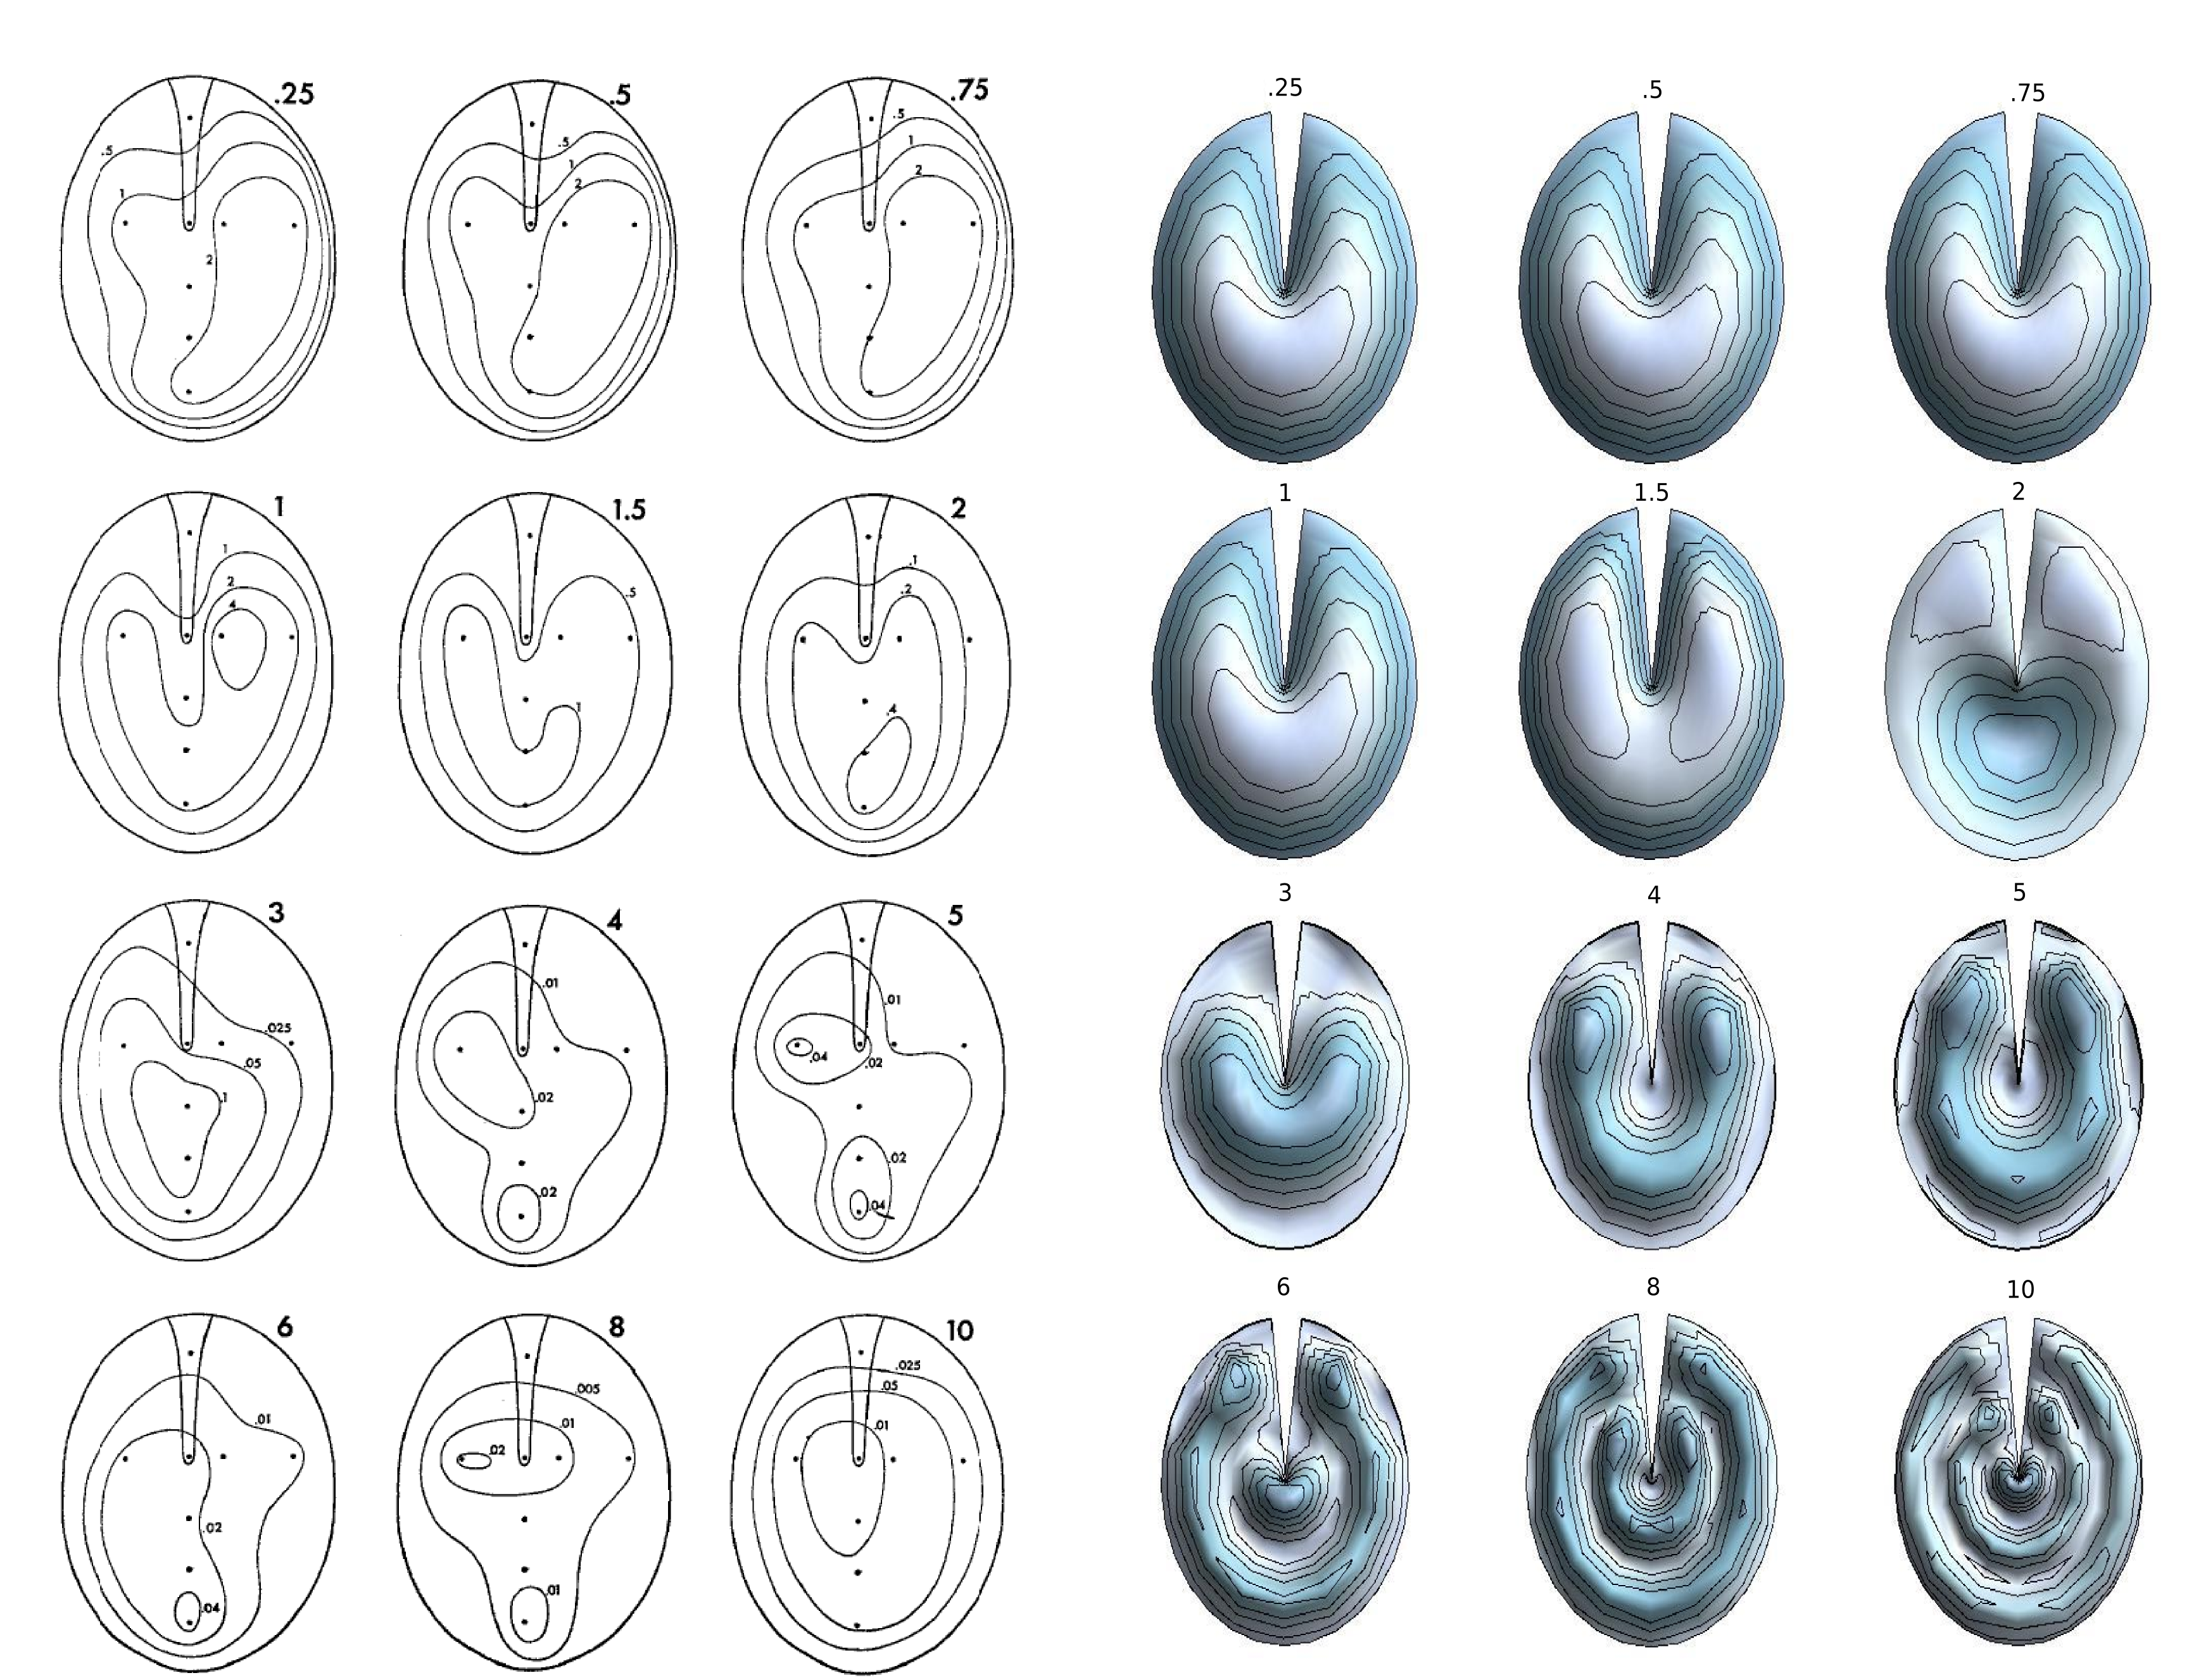
\includegraphics[width=1.0\linewidth]{Diagrams/manleymodelcomparison.png}
 \caption[Tympanic membrane vibration profiles for the Tokay gecko.]{Left: Experimental membrane vibration patterns of the Tokay gecko dependent
 on sound frequency varying from $.5$kHz to $10$kHz (corresponding frequency shown above membrane). Data taken from \cite{manleygecko1}. Right: Vibration
 pattern of one of the membranes in the ICE model with the opposite membrane blocked for the same frequency range. In both cases we see a similar
 complex vibrational pattern for the membranes which varies with frequency.}
  \label{manleygeckotympanum}
\end{figure}

In order to compare our model with the experimental results, we plot the response of one of the membranes ($x=0$, although $x=L$ could be
chosen equivalently due to the symmetry of the system) in our cylindrical ICE model 
calculated using \eqref{ipsimembranefull}. The opposite ear was chosen to be blocked, meaning $p_L=0$. 
This is illustrated in Fig. \ref{manleygeckotympanum} (right) for the same frequency range as in the experimental data. The sound pressure input was chosen to have unit amplitude and the model parameters used are given
on the right most column of Table \ref{geckogeometricparams}. The omitted region corresponds to the extracolumella. 

The asymmetric nature of our membrane vibration pattern is a result of our chosen geometry.
Mathematically this is a result of the fact that a uniform pressure (on the membrane surface) on a full circular membrane only couples to the circularly symmetric $J_0$ modes.
In the case of the sectoral membrane however, the uniform pressure couples to all the eigenmodes resulting in a more complex pattern.
As a qualitative reproduction our model is very accurate but for a full quantitative analysis, we would 
need to account for the motion of the extracolumella. Moreover, the full mechanics of the extracolumella including 
 its flection at higher frequencies can have significant effects which have not been studied so far.
% \begin{figure}[ht!]
%  \centering
%  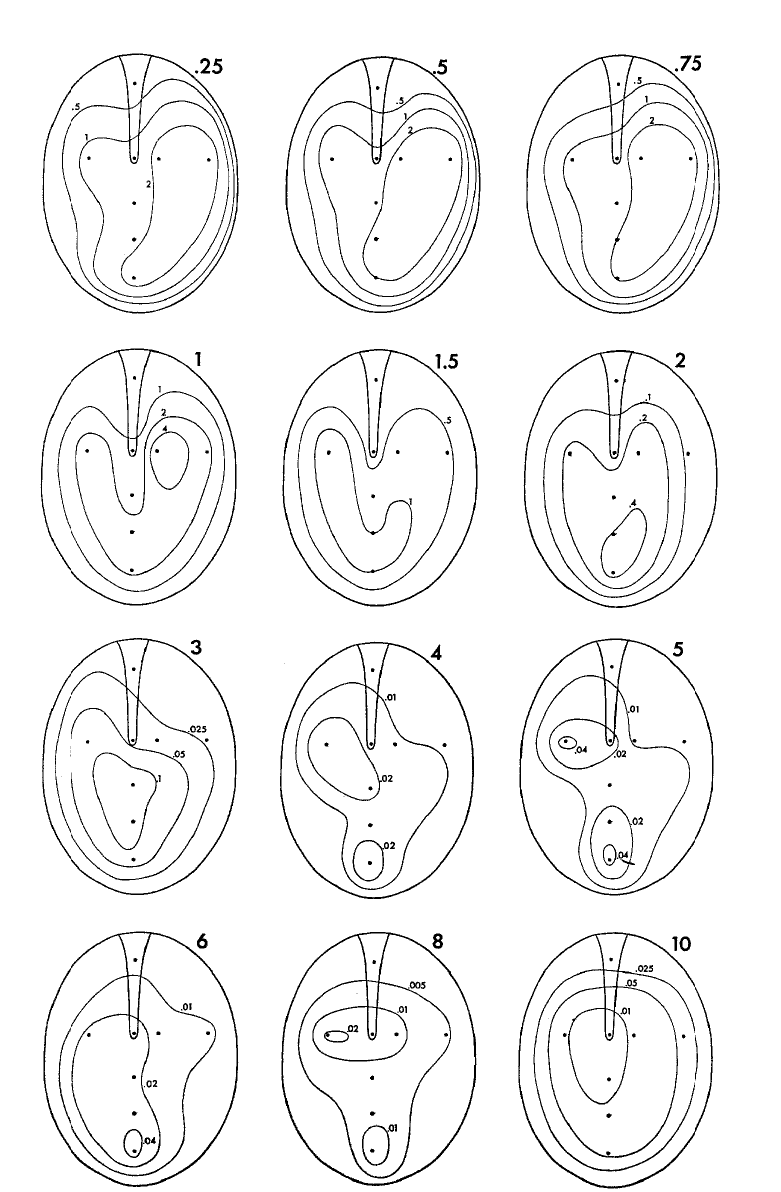
\includegraphics[width=.5\linewidth]{Diagrams/manleygeckoear2.png}
%  \caption[Tokay gecko tympanum vibration profiles.]{Experimental membrane vibration patterns of the Tokay gecko dependent
%  on sound frequency varying from $.5$kHz to $10$kHz. Data taken from \cite{manleygecko1}.}
%   \label{manleygeckotympanum}
% \end{figure}

% \begin{figure}[ht!]
%  \centering
%  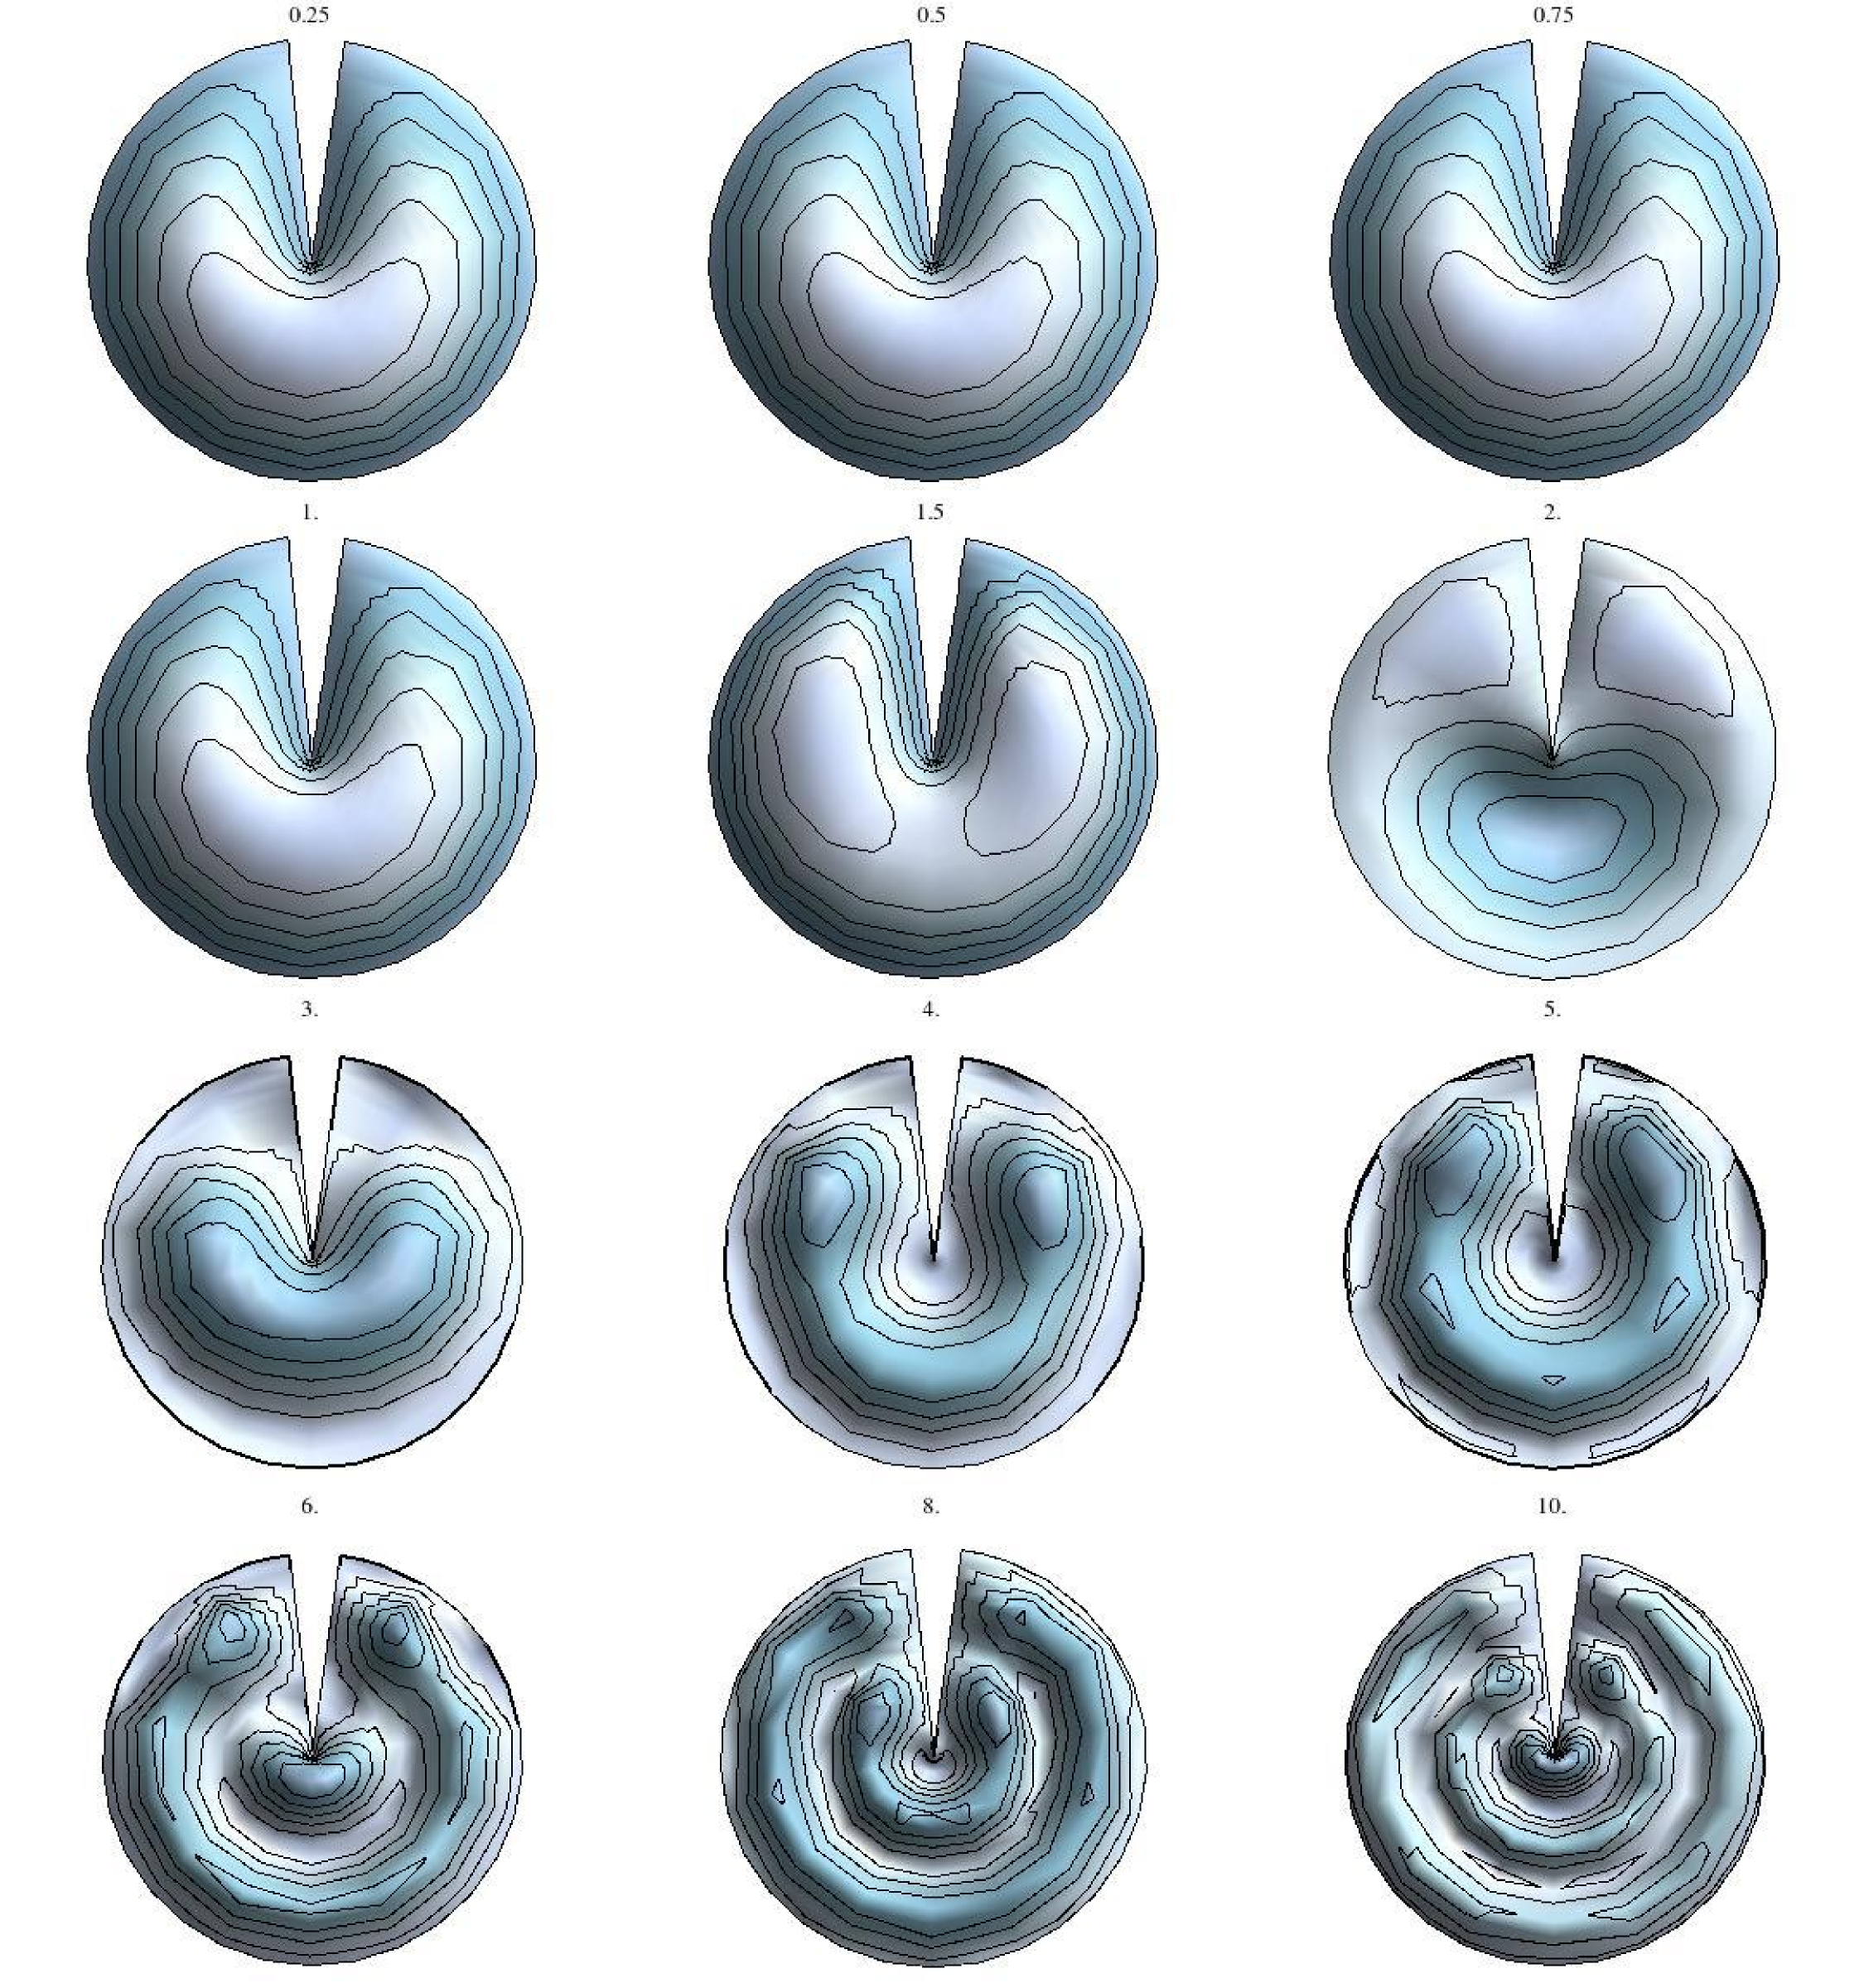
\includegraphics[width=.75\linewidth]{Diagrams/SectorMembraneModes/sector_membrane_all.png}
%  \caption[Sectoral membrane vibration profiles.]{Vibration patterns of a sectoral membrane
%  of radius $2.2$mm on sound frequency varying from $.5$kHz to $10$kHz. Compare with fig. \ref{manleygeckotympanum}}
%   \label{sectormembraneprofile}
% \end{figure}

  \chapter{Summary and Conclusion}
We started our study in Chapter \ref{modelchapter} by constructing a basic model that describes the motion of eardrums in animals
with coupled ears. The mouth cavity of the animal was modelled as an air-filled cylindrical tube
of radius $a_{cyl}$ with circular openings on either side of radius $a_{tymp}$ that are closed by
tympanic membranes of the same radius. This is one of the points where we deviate from the previous treatment
of the problem \cite{vossenjasa} as we have kept the volume of the cavity $V_{cav}$ constant and equal to
typical values for the species in nature. The sound inputs to both ears took the form of pressure waves
with a phase shift which depended on the frequency, direction of the source and head width and shape.

The second difference of our model from the previous treatment was the modelling of the membrane
as a circular sector of angle $2\pi-2\beta$. The remaining sector of angle $2\beta$ represented the 
the extracolumella - the extension whose function is to serve as a transducer of
membrane vibrations. We had modelled the extracolumella as being a stationary object and its
effect on the membranes was given through additional boundary conditions at $\phi=\pm\beta$. The variation of air-pressure
inside the tube was described by the $3D$ wave equation with no-penentration boundary conditions at the wall. In the previous
treatment it was assumed that the pressure modes inside the cavity are identical to the circular modes on the membrane. 

We then proceeded to find a solution to the full problem viz., the vibration of the membranes coupled through the cylindrical
cavity. This required the application of a new set of boundary conditions at the membrane-air interface. These conditions were
equivalent to the no-penetration boundary condition and required setting the membrane velocity to be equal to the velocity of
air inside the cavity. The complexity of these boundary conditions required an approximation. We expanded the membrane 
velocity in terms of the pressure modes and used the zeroeth order of the expansion. Thus we effectively approximated the membrane
by a piston oscillating with an amplitude equal to the integral of the membrane displacement. The approximation of the boundary
condition simplified the expression of the pressure by approximating it as a plane wave propagating along the $x$-axis. In the
frequency ranges of interest to us this turned out to be a reasonable assumption. At the end of the chapter we obtained expressions
for the membrane displacements in terms of the input pressure inputs to both ears.

In Chapter \ref{modelanalysis} we evalueated the results of our model - specifically its direction and frequency. We started
by comparing the total membrane displacements $S^{0/L}$ (the integrals of the membrane displacement) with the experimentally 
measured values of displacement at the tip of the extracolumella. 
For the membrane velocities, we found that they vary systematically with
direction and frequency and were in general higher in ipsilateral directions. The experimentally observed properties such
as the marked asymmetry, steepness across the midline and general frequency response were also reproduced. The shape of the membrane
velocities suggested that monoaural computation of membrane velocities would not serve well as directional cues.

We then went on to introduce the main directional cues in terms of the ratio $S^{0}$ and $S^{L}$. Namely, the Internal Level Difference
(iLD) which was defined as the decibel of the absolute value of this ratio and the Internal Time Difference (iTD) defined as its complex
argument divided by the angular frequency $\omega$. The simultaneous frequency and direction dependence of the iLD was illustrated by
means of contour plots and were found to be consistent with experimental measurements - both in terms of qualitative spectral behaviour and
quantitative values thus justifying our choice of $S^{0/L}$ as measures of membrane displacement. We then introduced the requirements these cues must fulfil in order to effectively serve as
directional cues. For the iLDs it was found that these requirements are best satisfied at relatively higher frequencies while
 iTDs seem to be more effective at lower frequencies. 
 
 The model thus inherently contains frequency regimes for both directional cues. While in the case of mammals the use of ITD/ILD
 is dictated by the size of the head in comparison to the wavelength, the transition in the ICE model is dictated my the membrane
 properties like the fundamental eigenfrequency and damping.
 




\section{Open Questions}
The main advantage of the ICE-model is to explain the frequency and direction dependence of the
hearing cues. In order to have a complete quantitative description of the ICE-model, we would also need to take
into account the motion of the extracolumella and the exact shape of realistic mouth cavities. The first of
these can be treated analytically upto a point. The main modification would be in the membrane boundary
conditions corresponding to the extracolumella. Instead of setting the displacement to zero, we would need to take into
account the mass of the extracolumella resulting in a new equation of motion. This equation would describe the motion
of the extracolumella driven by the membrane tension and the internal and external pressure difference. A further step
would be to incorporate the flection of the extracolumella at higher frequencies. This would require a further 
understanding of its constituent cartilaginous material and would necessitate a numerical treatment.

Due the complex shape of a realistic mouth cavity, a full treatment is not conducive to an analytical treatment.
Numerical software like COMSOL\textregistered can be used to treat reconstructions of mouth casts. Another possibility
would be to include the effects of the nostrils as either a new set of boundary conditions or a third input source.
%  \chapter{Das zweite Kapitel}

Dies ist das zweite Kapitel der Dissertation.


\section{Abschnitt Eins}

Dies ist der erste Abschnitt im zweiten Kapitel.


%%%%%%%%%%%%%%%%%%%%%%%%%%%%%%%%%%
%%  Beispiel fuer eine Tabelle  %%
%%%%%%%%%%%%%%%%%%%%%%%%%%%%%%%%%%

\begin{table}[htb]
\centering
\begin{tabular}{l|l}
Erste Spalte & Zweite Spalte \\ \hline
Eintrag & Eintrag
\end{tabular}
 \caption[Kurzform f"ur das Tabellenverzeichnis]{Dies ist die Erkl"arung zur Tabelle.}
\end{table}


\section{Abschnitt Zwei}

Jetzt kommt der zweite Abschnitt im zweiten Kapitel.

  %\include{kap_03}
  %\include{kap_04} usw.
  \begin{appendix}


% \chapter{Linear Acoustics}\label{acousticappendix}
% 
% Hier steht der erste Anhang.
% 
% 
% \chapter{Second Appendix Chapter}
% 
% Hier kommt der zweite Anhang.
\chapter{Mathematica Code}\label{codeappendix}
The Mathematica code used to calculate the total membrane displacements, iTD and iLD. The original input values are
for the Tokay gecko. The corresponding parameters for the house gecko are given in the comments.

% \begin{verbatim}
% Speciesname="Tokay";"or Hemidactylus";
% L:=22;"Cylinder Length in mm. 10/22";
% atymp:=2.6;"Radius of Tympanic Membrane in mm. 1.5/2.6";
% ρm=1;"1.25*.3125;" "Density of Membrane in mg/mm^3";
% d=.01; "Membrane Thickness in mm. .008/.01";
% β:=Pi/25; "Extracollumella angle";
% μ=Pi/(Pi-β);
% (*cM=25000;*)
% (*ρ=1.162*10^-3;"Density of Air mg/mm^3";*)
% V0=3500; "320/3500, mm^3";
% acyl=Sqrt[V0/(Pi*L)];
% "Volume of the Cylinder";
% γ=1.4;"Ratio of Specific Heats for Air";
% P0=101.325*10^6;"Atmospheric Pressure";
% (*c:=Sqrt[γ*P0/ρ];"Velocity of Sound mm/s";*)
% c=343000;
% ρ=γ*P0/c^2;"Density of Air mg/mm^3";
% f0=1050;"2800/1050";
% α=.9*2*Pi*f0/2.4; "Damping Coefficient of Membrane in Hz";
% ".75/.9" ;
% fmin=500;"Min hearing frequency - 1000 Hz for house gecko";
% fmax=3500;"Max Hearing Frequency - 7000Hz for house gecko";
% Out[529]= Maximum Hearing Frequency - 7000Hz for house gecko
% "Sound inputs to both ears";
% Φ=Pi*TriangleWave[θ/360]/2;
% ω=2*Pi*f;
% k=ω/c;
% p0=1000*E^(-.75*I*k*L*(Sin[θ Degree]));
% pL=1000*E^(.75*I*k*L*(Sin[θ Degree]));
% In[478]:= "Calculating and sorting the zeros of the membrane modes Bessel Functions";
% allZeros=Sort[Flatten[Table[{(l+.5)*μ,m,BesselJZero[(l+.5)*μ,m]/atymp},{l,0,9},{m,1,6}],1],(#1[[3]]<#2[[3]])&];
% In[480]:= "Membrane Propagation Velocity in terms of the first eigenfrequency mm/s";
% cM=f0*2*Pi/allZeros[[1]][[3]];
% Ncutoff=30; "Cutoff for the membrane modes";
% "Membrane impulse response";
% Λ=(Sum[Integrate[r*Sin[allZeros[[l]][[1]]*(ϕ-β)]*BesselJ[allZeros[[l]][[1]],allZeros[[l]][[3]]*r],{r,0,atymp},{ϕ,β,2*Pi-β}]^2/(ρm*d*(ω^2-2*I*α*ω-cM^2*allZeros[[l]][[3]]^2)*Integrate[r*Sin[allZeros[[l]][[1]]*(ϕ-β)]^2*BesselJ[allZeros[[l]][[1]],allZeros[[l]][[3]]*r]^2,{r,0,atymp},{ϕ,β,2*Pi-β}]),{l,1,Ncutoff}])^-1;
% 
% In[484]:= "Calculation of the total membrane displacements";
% Gamplus=-ρ*ω^2*Cot[k*L/2]/(Pi*acyl*acyl*k);
% Gamminus=ρ*ω^2*Tan[k*L/2]/(Pi*acyl*acyl*k);
% Splus=(pL+p0)/(Gamplus+Λ);
% Sminus=(pL-p0)/(Gamminus+Λ);
% SL=(Splus-Sminus)/2;
% S0=(Splus+Sminus)/2;
% In[491]:= "Internal Level Difference";
% iLD=20*Log10[Abs[S0/SL]];
% "Internal Time Difference";
% iTD=Arg[S0/SL]/ω;
% In[530]:= "Density Plot of Membrane Vibration Amplitude";
% dticks=Table[{(l-1)*90-180,ToString[(l-1)*90-180],{0,.01}},{l,1,5}];
% fticks=Table[{l*fmin,ToString[l*fmin],{0,.01}},{l,1,7}];
% ShowLegend[DensityPlot[20*Log10[ω*Abs[S0]/(Pi*acyl*acyl)],{θ,-180,180},{f,fmin,fmax},ColorFunction->"BlueGreenYellow",PlotPoints->20,Frame->False,Axes->True,AxesOrigin->{-180,200},AxesLabel->{None,"frequency (Hz)"},Ticks->{dticks,fticks},PlotLabel->Speciesname,FrameLabel->{"direction(degrees)",None}],{ColorData["BlueGreenYellow"][#1]&,8,"-30","10",LegendPosition->{-1.5,-.35},LegendOrientation->Vertical}]
% "Membrane vibration spectrum for different source directions";
% dbticks=Table[{(l-1)*10-40,ToString[(l-1)*10-40],{0,.005}},{l,1,6}];Plot[{20*Log10[ω*Abs[S0]/(Pi*acyl*acyl)]/.θ->90,20*Log10[ω*Abs[S0]/(Pi*acyl*acyl)]/.θ->60,20*Log10[ω*Abs[S0]/(Pi*acyl*acyl)]/.θ->0,20*Log10[ω*Abs[S0]/(Pi*acyl*acyl)]/.θ->-60,20*Log10[ω*Abs[S0]/(Pi*acyl*acyl)]/.θ->-90},{f,fmin,fmax},PlotRange->{-40,10},PlotStyle->{ColorData[1][1],ColorData[1][2],Dotted,Dashed,Dashed},AxesOrigin->{500,-40},PlotLabel->"Tokay",Epilog->{Line[{{5000,-40},{5000,10},{500,10},{5000,10}}]},Ticks->{fticks,dbticks},PlotLegend->{"90°","60°","0°","-60°","-90°"},LegendPosition->{.9,-.4}]
% "Membrane vibration direction dependence";
% ftest=1000; "Test Frequency - refer Chapter 3 for values";
% mrange=Floor[-10+20*Log10[ω*Abs[S0]/(Pi*acyl*acyl)]/.{f->ftest,θ->-90}];
% prange=Ceiling[10+20*Log10[ω*Abs[S0]/(Pi*acyl*acyl)]/.{f->ftest,θ->90}];
% dticks=Table[{(l-1)*90-180,ToString[(l-1)*90-180],{0,.01}},{l,1,5}];
% ndbticks=5;
% dbticks=Table[{(l-1)*(prange-mrange)/(ndbticks-1)+mrange,ToString[(l-1)*(prange-mrange)/(ndbticks-1)+mrange],{0,.005}},{l,1,ndbticks}];
% Plot[20*Log10[ω*Abs[S0]/(Pi*acyl*acyl)]/.f->ftest,{θ,-180,180},PlotRange->{mrange,prange},PlotStyle->Black,AxesOrigin->{-180,mrange},PlotLabel->ToString[ftest]<>"Hz",Ticks->{dticks,dbticks},Epilog->{Line[{{180,mrange},{180,prange},{-180,prange},{180,prange}}]}]
% \end{verbatim}
\begin{doublespace}
\noindent\(\pmb{\text{Speciesname}=\text{{``}Tokay{''}};\text{{``}or Hemidactylus{''}};}\\
\pmb{L\text{:=}22;\text{{``}Cylinder Length in mm. 10/22{''}};}\\
\pmb{\text{atymp}\text{:=}2.6;\text{{``}Radius of Tympanic Membrane in mm. 1.5/2.6{''}};}\\
\pmb{\text{$\rho $m}=1;\text{{``}1.25*.3125;{''}} \text{{``}Density of Membrane in mg/mm${}^{\wedge}$3{''}};}\\
\pmb{d=.01; \text{{``}Membrane Thickness in mm. .008/.01{''}};}\\
\pmb{\beta \text{:=}\text{Pi}/25; \text{{``}Extracollumella angle{''}};}\\
\pmb{\mu =\text{Pi}/(\text{Pi}-\beta );}\\
\pmb{\text{(*}\text{cM}=25000;\text{*)}}\\
\pmb{\text{(*}\rho =1.162*10{}^{\wedge}-3;\text{{``}Density of Air mg/mm${}^{\wedge}$3{''}};\text{*)}}\\
\pmb{\text{V0}=3500; \text{{``}320/3500, mm${}^{\wedge}$3{''}};}\\
\pmb{\text{acyl}=\text{Sqrt}[\text{V0}/(\text{Pi}*L)];}\\
\pmb{\text{{``}Volume of the Cylinder{''}};}\\
\pmb{\gamma =1.4;\text{{``}Ratio of Specific Heats for Air{''}};}\\
\pmb{\text{P0}=101.325*10{}^{\wedge}6;\text{{``}Atmospheric Pressure{''}};}\\
\pmb{\text{(*}c\text{:=}\text{Sqrt}[\gamma *\text{P0}/\rho ];\text{{``}Velocity of Sound mm/s{''}};\text{*)}}\\
\pmb{c=343000;}\\
\pmb{\rho =\gamma *\text{P0}/c{}^{\wedge}2;\text{{``}Density of Air mg/mm${}^{\wedge}$3{''}};}\\
\pmb{\text{f0}=1050;\text{{``}2800/1050{''}};}\\
\pmb{\alpha =.9*2*\text{Pi}*\text{f0}/2.4; \text{{``}Damping Coefficient of Membrane in Hz{''}};}\)
\end{doublespace}

\begin{doublespace}
\noindent\(\pmb{\text{{``}Sound inputs to both ears{''}};}\\
\pmb{\Phi =\text{Pi}*\text{TriangleWave}[\theta /360]/2;}\\
\pmb{\omega =2*\text{Pi}*f;}\\
\pmb{k=\omega /c;}\\
\pmb{\text{p0}=1000*E{}^{\wedge}(-.75*I*k*L*(\text{Sin}[\theta  \text{Degree}]));\text{{``}Pressure is 1Pa in units of mg/(mm s${}^{\wedge}$2){''}};}\\
\pmb{\text{pL}=1000*E{}^{\wedge}(.75*I*k*L*(\text{Sin}[\theta  \text{Degree}]));}\)
\end{doublespace}

\begin{doublespace}
\noindent\(\pmb{\text{{``}Calculating and sorting the zeros of the membrane modes Bessel Functions{''}};}\\
\pmb{\text{allZeros}=\text{Sort}[\text{Flatten}[\text{Table}[\{(l+.5)*\mu ,m,\text{BesselJZero}[(l+.5)*\mu ,m]/\text{atymp}\},\{l,0,9\},\{m,1,6\}],1],}\\
\pmb{(\text{$\#$1}[[3]]<\text{$\#$2}[[3]])\&];}\)
\end{doublespace}

\begin{doublespace}
\noindent\(\pmb{\text{{``}Membrane Propagation Velocity in terms of the first eigenfrequency mm/s{''}};}\\
\pmb{\text{cM}=\text{f0}*2*\text{Pi}/\text{allZeros}[[1]][[3]];}\)
\end{doublespace}

\begin{doublespace}
\noindent\(\pmb{\text{Ncutoff}=30; \text{{``}Cutoff for the membrane modes{''}};}\\
\pmb{\text{{``}Membrane impulse response{''}};}\\
\pmb{\Lambda =}\\
\pmb{(\text{Sum}[\text{Integrate}[r*\text{Sin}[\text{allZeros}[[l]][[1]]*(\phi -\beta )]*\text{BesselJ}[\text{allZeros}[[l]][[1]],\text{allZeros}[[l]][[3]]*r],}\\
\pmb{\{r,0,\text{atymp}\},\{\phi ,\beta ,2*\text{Pi}-\beta \}]{}^{\wedge}2/}\\
\pmb{(\text{$\rho $m}*d*(\omega {}^{\wedge}2-2*I*\alpha *\omega -\text{cM}{}^{\wedge}2*\text{allZeros}[[l]][[3]]{}^{\wedge}2)*}\\
\pmb{\text{Integrate}[r*\text{Sin}[\text{allZeros}[[l]][[1]]*(\phi -\beta )]{}^{\wedge}2*}\\
\pmb{\text{BesselJ}[\text{allZeros}[[l]][[1]],\text{allZeros}[[l]][[3]]*r]{}^{\wedge}2,\{r,0,\text{atymp}\},\{\phi ,\beta ,2*\text{Pi}-\beta \}]),}\\
\pmb{\{l,1,\text{Ncutoff}\}]){}^{\wedge}-1;}\)
\end{doublespace}

\begin{doublespace}
\noindent\(\pmb{\text{{``}Calculation of the total membrane displacements{''}};}\\
\pmb{\text{Gamplus}=-\rho *\omega {}^{\wedge}2*\text{Cot}[k*L/2]/(\text{Pi}*\text{acyl}*\text{acyl}*k);}\\
\pmb{\text{Gamminus}=\rho *\omega {}^{\wedge}2*\text{Tan}[k*L/2]/(\text{Pi}*\text{acyl}*\text{acyl}*k);}\\
\pmb{\text{Splus}=(\text{pL}+\text{p0})/(\text{Gamplus}+\Lambda );}\\
\pmb{\text{Sminus}=(\text{pL}-\text{p0})/(\text{Gamminus}+\Lambda );}\\
\pmb{\text{SL}=(\text{Splus}-\text{Sminus})/2;}\\
\pmb{\text{S0}=(\text{Splus}+\text{Sminus})/2;}\)
\end{doublespace}

\begin{doublespace}
\noindent\(\pmb{\text{{``}Internal Level Difference{''}};}\\
\pmb{\text{iLD}=20*\text{Log10}[\text{Abs}[\text{S0}/\text{SL}]];}\\
\pmb{\text{{``}Internal Time Difference{''}};}\\
\pmb{\text{iTD}=\text{Arg}[\text{S0}/\text{SL}]/\omega ;}\)
\end{doublespace}

\begin{doublespace}
\noindent\(\pmb{\text{Needs}[\text{{``}PlotLegends$\grave{ }${''}}];}\)
\end{doublespace}

\begin{doublespace}
\noindent\(\pmb{\text{{``}Plot ticks for direction and frequency{''}};}\\
\pmb{\text{dticks}=\text{Table}[\{(l-1)*90-180,\text{ToString}[(l-1)*90-180],\{0,.01\}\},\{l,1,5\}];}\\
\pmb{\text{fticks}=\text{Table}[\{l*\text{fmin},\text{ToString}[l*\text{fmin}],\{0,.01\}\},\{l,1,7\}];}\)
\end{doublespace}

\begin{doublespace}
\noindent\(\pmb{\text{{``}Density Plot of Membrane Vibration Amplitude{''}};}\\
\pmb{\text{ShowLegend}[\text{DensityPlot}[20*\text{Log10}[\omega *\text{Abs}[\text{S0}]/(\text{Pi}*\text{acyl}*\text{acyl})],\{\theta ,-180,180\},\{f,\text{fmin},\text{fmax}\},}\\
\pmb{\text{ColorFunction}\to \text{{``}BlueGreenYellow{''}},\text{PlotPoints}\to 20,\text{Frame}\to \text{False},\text{Axes}\to \text{True},}\\
\pmb{\text{AxesOrigin}\to \{-180,200\},\text{AxesLabel}\to \{\text{None},\text{{``}frequency (Hz){''}}\},\text{Ticks}\to \{\text{dticks},\text{fticks}\},}\\
\pmb{\text{PlotLabel}\to \text{Speciesname},\text{FrameLabel}\to \{\text{{``}direction(degrees){''}},\text{None}\}],}\\
\pmb{\{\text{ColorData}[\text{{``}BlueGreenYellow{''}}][\text{$\#$1}]\&,8,\text{{``}-30{''}},\text{{``}10{''}},\text{LegendPosition}\to \{-1.5,-.35\},}\\
\pmb{\text{LegendOrientation}\to \text{Vertical}\}]}\)
\end{doublespace}

\begin{doublespace}
\noindent\(\pmb{\text{{``}Membrane vibration spectrum for different source directions{''}};}\\
\pmb{\text{dbticks}=\text{Table}[\{(l-1)*10-40,\text{ToString}[(l-1)*10-40],\{0,.005\}\},\{l,1,6\}];}\\
\pmb{\text{Plot}[\{20*\text{Log10}[\omega *\text{Abs}[\text{S0}]/(\text{Pi}*\text{acyl}*\text{acyl})]\text{/.}\theta \to 90,20*\text{Log10}[\omega
*\text{Abs}[\text{S0}]/(\text{Pi}*\text{acyl}*\text{acyl})]\text{/.}\theta \to 60,}\\
\pmb{20*\text{Log10}[\omega *\text{Abs}[\text{S0}]/(\text{Pi}*\text{acyl}*\text{acyl})]\text{/.}\theta \to 0,20*\text{Log10}[\omega *\text{Abs}[\text{S0}]/(\text{Pi}*\text{acyl}*\text{acyl})]\text{/.}\theta
\to -60,}\\
\pmb{20*\text{Log10}[\omega *\text{Abs}[\text{S0}]/(\text{Pi}*\text{acyl}*\text{acyl})]\text{/.}\theta \to -90\},\{f,\text{fmin},\text{fmax}\},\text{PlotRange}\to
\{-40,10\},}\\
\pmb{\text{PlotStyle}\to \{\text{ColorData}[1][1],\text{ColorData}[1][2],\text{Dotted},\text{Dashed},\text{Dashed}\},\text{AxesOrigin}\to \{500,-40\},}\\
\pmb{\text{PlotLabel}\to \text{{``}Tokay{''}},\text{Epilog}\to \{\text{Line}[\{\{5000,-40\},\{5000,10\},\{500,10\},\{5000,10\}\}]\},}\\
\pmb{\text{Ticks}\to \{\text{fticks},\text{dbticks}\},\text{PlotLegend}\to \{\text{{``}90${}^{\circ}${''}},\text{{``}60${}^{\circ}${''}},\text{{``}0${}^{\circ}${''}},\text{{``}-60${}^{\circ}${''}},\text{{``}-90${}^{\circ}${''}}\},\text{LegendPosition}\to
\{.9,-.4\}]}\)
\end{doublespace}

\begin{doublespace}
\noindent\(\pmb{\text{{``}Membrane vibration direction dependence{''}};}\\
\pmb{\text{ftest}=1000; \text{{``}Test Frequency - refer Chapter 3 for values{''}};}\\
\pmb{\text{mrange}=\text{Floor}[-10+20*\text{Log10}[\omega *\text{Abs}[\text{S0}]/(\text{Pi}*\text{acyl}*\text{acyl})]\text{/.}\{f\to \text{ftest},\theta
\to -90\}];}\\
\pmb{\text{prange}=\text{Ceiling}[10+20*\text{Log10}[\omega *\text{Abs}[\text{S0}]/(\text{Pi}*\text{acyl}*\text{acyl})]\text{/.}\{f\to \text{ftest},\theta
\to 90\}];}\\
\pmb{\text{ndbticks}=5;}\\
\pmb{\text{dbticks}=}\\
\pmb{\text{Table}[\{(l-1)*(\text{prange}-\text{mrange})/(\text{ndbticks}-1)+\text{mrange},}\\
\pmb{\text{ToString}[N[(l-1)*(\text{prange}-\text{mrange})/(\text{ndbticks}-1)+\text{mrange}]],\{0,.005\}\},\{l,1,\text{ndbticks}\}];}\\
\pmb{\text{Plot}[20*\text{Log10}[\omega *\text{Abs}[\text{S0}]/(\text{Pi}*\text{acyl}*\text{acyl})]\text{/.}f\to \text{ftest},\{\theta ,-180,180\},\text{PlotRange}\to
\{\text{mrange},\text{prange}\},}\\
\pmb{\text{PlotStyle}\to \text{Black},\text{AxesOrigin}\to \{-180,\text{mrange}\},\text{PlotLabel}\to \text{ToString}[\text{ftest}]<>\text{{``}Hz{''}},}\\
\pmb{\text{Ticks}\to \{\text{dticks},\text{dbticks}\},\text{Epilog}\to \{\text{Line}[\{\{180,\text{mrange}\},\{180,\text{prange}\},\{-180,\text{prange}\},\{180,\text{prange}\}\}]\}]}\)
\end{doublespace}

\begin{doublespace}
\noindent\(\pmb{\text{{``}iLD with respect to direction and frequency{''}};}\\
\pmb{\text{range}=15+20*\text{Log10}[\text{Abs}[\text{S0}/\text{SL}]]\text{/.}\{f\to \text{f0},\theta \to 90\};}\\
\pmb{\text{ShowLegend}[\text{ContourPlot}[20*\text{Log10}[\text{Abs}[\text{S0}/\text{SL}]],\{\theta ,-180,180\},\{f,\text{fmin},\text{fmax}\},}\\
\pmb{\text{ColorFunction}\to \text{{``}BlueGreenYellow{''}},\text{PlotPoints}\to 20,\text{Contours}\to 20,\text{Frame}\to \text{False},\text{Axes}\to
\text{True},}\\
\pmb{\text{PlotRange}\to \text{range},\text{AxesOrigin}\to \{-180,200\},\text{AxesLabel}\to \{\text{None},\text{{``}frequency (Hz){''}}\},}\\
\pmb{\text{Ticks}\to \{\text{dticks},\text{fticks}\},\text{PlotLabel}\to \text{Speciesname},\text{FrameLabel}\to \{\text{{``}direction(degrees){''}},\text{None}\}],}\\
\pmb{\{\text{ColorData}[\text{{``}BlueGreenYellow{''}}][\text{$\#$1}]\&,8,\text{{``}-30{''}},\text{{``}10{''}},\text{LegendPosition}\to \{-1.5,-.35\},}\\
\pmb{\text{LegendOrientation}\to \text{Vertical}\}]}\)
\end{doublespace}

\begin{doublespace}
\noindent\(\pmb{\text{}}\\
\pmb{\text{{``}iLD direction dependence{''}};}\\
\pmb{\text{ftest}=1000; \text{{``}Test Frequency - refer Chapter 3 for values{''}};}\\
\pmb{\text{mrange}=\text{Floor}[-10+20*\text{Log10}[\text{Abs}[\text{S0}/\text{SL}]]\text{/.}\{f\to \text{ftest},\theta \to -90\}];}\\
\pmb{\text{prange}=\text{Ceiling}[10+20*\text{Log10}[\text{Abs}[\text{S0}/\text{SL}]]\text{/.}\{f\to \text{ftest},\theta \to 90\}];}\\
\pmb{\text{ndbticks}=5;}\\
\pmb{\text{dbticks}=}\\
\pmb{\text{Table}[\{(l-1)*(\text{prange}-\text{mrange})/(\text{ndbticks}-1)+\text{mrange},}\\
\pmb{\text{ToString}[N[(l-1)*(\text{prange}-\text{mrange})/(\text{ndbticks}-1)+\text{mrange}]],\{0,.005\}\},\{l,1,\text{ndbticks}\}];}\\
\pmb{\text{Plot}[20*\text{Log10}[\text{Abs}[\text{S0}/\text{SL}]]\text{/.}f\to \text{ftest},\{\theta ,-180,180\},\text{PlotRange}\to \{\text{mrange},\text{prange}\},}\\
\pmb{\text{PlotStyle}\to \text{Black},\text{AxesOrigin}\to \{-180,\text{mrange}\},\text{PlotLabel}\to \text{ToString}[\text{ftest}]<>\text{{``}Hz{''}},}\\
\pmb{\text{Ticks}\to \{\text{dticks},\text{dbticks}\},\text{Epilog}\to \{\text{Line}[\{\{180,\text{mrange}\},\{180,\text{prange}\},\{-180,\text{prange}\},\{180,\text{prange}\}\}]\}]}\)
\end{doublespace}

\begin{doublespace}
\noindent\(\pmb{\text{{``}iLD spectrum with directional bandwidth{''}};}\\
\pmb{\text{ndbticks}=5;}\\
\pmb{\text{dbticks}=\text{Table}[\{(l-1)*40/(\text{ndbticks}-1),\text{ToString}[N[(l-1)*40/(\text{ndbticks}-1)]],\{0,.005\}\},}\\
\pmb{\{l,1,\text{ndbticks}\}];}\\
\pmb{\text{Plot}[\{20*\text{Log10}[\text{Abs}[\text{S0}/\text{SL}]]\text{/.}\{\theta \to 90\},\text{If}[(20*\text{Log10}[\text{Abs}[\text{S0}/\text{SL}]]\text{/.}\{\theta
\to 90\})>3,3]\},}\\
\pmb{\{f,\text{fmin},\text{fmax}\},\text{PlotRange}\to \{0,40\},\text{PlotStyle}\to \{\text{Black},\text{None}\},\text{Ticks}\to \{\text{fticks},\text{dbticks},\text{None},\text{None}\},}\\
\pmb{\text{AxesOrigin}\to \{\text{fmin},0\},\text{Filling}\to \{1\to \{2\}\},\text{Epilog}\to \{\text{Line}[\{\{\text{fmin},40\},\{\text{fmax},40\},\{\text{fmax},0\},\{\text{fmax},40\}\}]\}]}\)
\end{doublespace}

\begin{doublespace}
\noindent\(\pmb{\text{{``}iTD spectrum{''}};}\\
\pmb{\text{Tmax}=\text{Round}[6*L*10{}^{\wedge}6/c,50];}\\
\pmb{\text{ntticks}=6;}\\
\pmb{\text{tticks}=\text{Table}[\{(l-1)*\text{Tmax}/(\text{ntticks}-1),\text{ToString}[N[(l-1)*\text{Tmax}/(\text{ntticks}-1)]],\{0,.005\}\},}\\
\pmb{\{l,1,\text{ntticks}\}];}\\
\pmb{\text{Plot}[\{10{}^{\wedge}6*\text{Arg}[\text{S0}/\text{SL}]/\omega \text{/.}\theta \to 90\},\{f,\text{fmin},\text{fmax}\},\text{PlotRange}\to
\{-40,\text{Tmax}\},\text{AxesOrigin}\to \{\text{fmin},0\},}\\
\pmb{\text{Ticks}\to \{\text{fticks},\text{tticks}\},\text{PlotRange}\to \text{All},\text{PlotStyle}\to \text{Black}]}\)
\end{doublespace}

\begin{doublespace}
\noindent\(\pmb{\text{{``}iTD direction dependence{''}};}\\
\pmb{\text{ftest1}=1000;}\\
\pmb{\text{ntticks}=9;}\\
\pmb{\text{tticks}=\text{Table}[\{-\text{Tmax}+2*(l-1)*\text{Tmax}/(\text{ntticks}-1),\text{ToString}[N[-\text{Tmax}+2*(l-1)*\text{Tmax}/(\text{ntticks}-1)]],}\\
\pmb{\{0,.005\}\},\{l,1,\text{ntticks}\}];}\\
\pmb{\text{Plot}[\{10{}^{\wedge}6*\text{Arg}[\text{SL}/\text{S0}]/\omega \text{/.}f\to \text{ftest1},10{}^{\wedge}6*\text{Arg}[\text{SL}/\text{S0}]/\omega
\text{/.}f\to 2*\text{ftest1},}\\
\pmb{10{}^{\wedge}6*\text{Arg}[\text{SL}/\text{S0}]/\omega \text{/.}f\to 3*\text{ftest1}\},\{\theta ,-180,180\},\text{PlotRange}\to \text{Tmax},\text{PlotStyle}\to
\{\text{Black},\text{Red},\text{Green}\},}\\
\pmb{\text{AxesOrigin}\to \{-180,-\text{Tmax}\},\text{Ticks}\to \{\text{dticks},\text{tticks}\},}\\
\pmb{\text{Epilog}\to \{\text{Line}[\{\{-180,0\},\{180,0\},\{180,-\text{Tmax}\},\{180,\text{Tmax}\},\{-180,\text{Tmax}\},\{180,\text{Tmax}\}\}]\},}\\
\pmb{\text{PlotLegend}\to \{\text{Style}[\text{{``}1kHz{''}},\text{Black},18],\text{Style}[\text{{``}2kHz{''}},\text{Black},18],\text{Style}[\text{{``}3kHz{''}},\text{Black},18]\},}\\
\pmb{\text{LegendPosition}\to \{-2.0,-.25\}]}\)
\end{doublespace}

\begin{doublespace}
\noindent\(\pmb{\text{}}\)
\end{doublespace}

\begin{doublespace}
\noindent\(\pmb{\text{{``}Membrane Vibration Profile{''}};}\\
\pmb{\text{membamp}=}\\
\pmb{\text{Sum}[\text{Integrate}[r*\text{Sin}[\text{allZeros}[[l]][[1]]*(\phi -\beta )]*\text{BesselJ}[\text{allZeros}[[l]][[1]],\text{allZeros}[[l]][[3]]*r],}\\
\pmb{\{r,0,\text{atymp}\},\{\phi ,\beta ,2*\text{Pi}-\beta \}]*\text{Sin}[\text{allZeros}[[l]][[1]]*(\phi -\beta )]*}\\
\pmb{\text{BesselJ}[\text{allZeros}[[l]][[1]],\text{allZeros}[[l]][[3]]*r]/}\\
\pmb{(\text{$\rho $m}*d*(\omega {}^{\wedge}2-2*I*\alpha *\omega -\text{cM}{}^{\wedge}2*\text{allZeros}[[l]][[3]]{}^{\wedge}2)*}\\
\pmb{\text{Integrate}[r*\text{Sin}[\text{allZeros}[[l]][[1]]*(\phi -\beta )]{}^{\wedge}2*}\\
\pmb{\text{BesselJ}[\text{allZeros}[[l]][[1]],\text{allZeros}[[l]][[3]]*r]{}^{\wedge}2,\{r,0,\text{atymp}\},\{\phi ,\beta ,2*\text{Pi}-\beta \}]),}\\
\pmb{\{l,1,\text{Ncutoff}\}];}\\
\pmb{\text{ipsimemb}=\Lambda *\text{membamp}*(1/(\text{Gamplus}+\Lambda )+1/(\text{Gamminus}+\Lambda ));}\\
\pmb{\text{flist}=\{250,500,750,1000,1500,2000,3000,4000,5000,6000,8000,10000\};}\\
\pmb{\text{ftest}=\text{flist}[[1]];}\\
\pmb{\text{membplot}=\text{Re}[\text{ipsimemb}\text{/.}f\to \text{ftest}];}\\
\pmb{\text{RevolutionPlot3D}[\text{membplot},\{r,0,\text{atymp}\},\{\phi ,\beta ,2*\text{Pi}-\beta \},}\\
\pmb{\text{ColorFunction}\to \text{Function}[\{x,y,z,t,\theta ,r\},\text{ColorData}[\text{{``}Aquamarine{''}}][z]],}\\
\pmb{\text{MeshFunctions}\to \{\text{Function}[\{x,y,z,t,\theta ,r\},\text{Evaluate}[z]]\},\text{MeshStyle}\to \text{Thick},\text{Mesh}\to 8,}\\
\pmb{\text{Boxed}\to \text{False},\text{Axes}\to \text{False},\text{PlotLabel}\to \text{Style}[\text{ToString}[N[\text{ftest}/1000]],24]]}\)
\end{doublespace}

\end{appendix}



  \backmatter
  %\bibliographystyle{jkthesis}

\bibliographystyle{apalike}
\bibliography{literatur}

  \markboth{}{}


  \addcontentsline{toc}{chapter}{\protect Acknowledgements}

\begin{quotation} 
\centering
\noindent \emph{Work It Harder Make It Better}

\emph{Do It Faster, Makes Us stronger}

\emph{More Than Ever Hour After}

\emph{Our Work Is Never Over.}
\flushright Daft Punk
\flushright Discovery (2001)
\end{quotation}

\chapter*{Acknowledgements}
I should and will begin by thanking my advisor Prof. Dr. J. Leo van Hemmen
for introducing me to the far from uninteresting world of lizards and
the clever things they do to figure out what's what and who's where. His combination
of patience and enthusiasm was indispensable. The same can, should and will be said
about Dr. Julie Goulet without whose guidance this thesis would be short by about 80
pages.



%  \chapter*{Lebenslauf}

Sigmund Stintzing

\vspace*{2.0cm}

\begin{tabular}{ll}

Geburtsdatum & Geburt in Geburtsort \\[1.5ex]
Schulzeit & Besuch der Schule in Ort \\[1.5ex]
 ... & ...
\end{tabular}



\end{document}
